% Options for packages loaded elsewhere
% Options for packages loaded elsewhere
\PassOptionsToPackage{unicode}{hyperref}
\PassOptionsToPackage{hyphens}{url}
\PassOptionsToPackage{dvipsnames,svgnames,x11names}{xcolor}
%
\documentclass[
  12pt,
]{article}
\usepackage{xcolor}
\usepackage[margin=2cm]{geometry}
\usepackage{amsmath,amssymb}
\setcounter{secnumdepth}{5}
\usepackage{iftex}
\ifPDFTeX
  \usepackage[T1]{fontenc}
  \usepackage[utf8]{inputenc}
  \usepackage{textcomp} % provide euro and other symbols
\else % if luatex or xetex
  \usepackage{unicode-math} % this also loads fontspec
  \defaultfontfeatures{Scale=MatchLowercase}
  \defaultfontfeatures[\rmfamily]{Ligatures=TeX,Scale=1}
\fi
\usepackage{lmodern}
\ifPDFTeX\else
  % xetex/luatex font selection
  \setmainfont[]{Times New Roman}
\fi
% Use upquote if available, for straight quotes in verbatim environments
\IfFileExists{upquote.sty}{\usepackage{upquote}}{}
\IfFileExists{microtype.sty}{% use microtype if available
  \usepackage[]{microtype}
  \UseMicrotypeSet[protrusion]{basicmath} % disable protrusion for tt fonts
}{}
\usepackage{setspace}
\makeatletter
\@ifundefined{KOMAClassName}{% if non-KOMA class
  \IfFileExists{parskip.sty}{%
    \usepackage{parskip}
  }{% else
    \setlength{\parindent}{0pt}
    \setlength{\parskip}{6pt plus 2pt minus 1pt}}
}{% if KOMA class
  \KOMAoptions{parskip=half}}
\makeatother
% Make \paragraph and \subparagraph free-standing
\makeatletter
\ifx\paragraph\undefined\else
  \let\oldparagraph\paragraph
  \renewcommand{\paragraph}{
    \@ifstar
      \xxxParagraphStar
      \xxxParagraphNoStar
  }
  \newcommand{\xxxParagraphStar}[1]{\oldparagraph*{#1}\mbox{}}
  \newcommand{\xxxParagraphNoStar}[1]{\oldparagraph{#1}\mbox{}}
\fi
\ifx\subparagraph\undefined\else
  \let\oldsubparagraph\subparagraph
  \renewcommand{\subparagraph}{
    \@ifstar
      \xxxSubParagraphStar
      \xxxSubParagraphNoStar
  }
  \newcommand{\xxxSubParagraphStar}[1]{\oldsubparagraph*{#1}\mbox{}}
  \newcommand{\xxxSubParagraphNoStar}[1]{\oldsubparagraph{#1}\mbox{}}
\fi
\makeatother


\usepackage{longtable,booktabs,array}
\newcounter{none} % for unnumbered tables
\usepackage{calc} % for calculating minipage widths
% Correct order of tables after \paragraph or \subparagraph
\usepackage{etoolbox}
\makeatletter
\patchcmd\longtable{\par}{\if@noskipsec\mbox{}\fi\par}{}{}
\makeatother
% Allow footnotes in longtable head/foot
\IfFileExists{footnotehyper.sty}{\usepackage{footnotehyper}}{\usepackage{footnote}}
\makesavenoteenv{longtable}
\usepackage{graphicx}
\makeatletter
\newsavebox\pandoc@box
\newcommand*\pandocbounded[1]{% scales image to fit in text height/width
  \sbox\pandoc@box{#1}%
  \Gscale@div\@tempa{\textheight}{\dimexpr\ht\pandoc@box+\dp\pandoc@box\relax}%
  \Gscale@div\@tempb{\linewidth}{\wd\pandoc@box}%
  \ifdim\@tempb\p@<\@tempa\p@\let\@tempa\@tempb\fi% select the smaller of both
  \ifdim\@tempa\p@<\p@\scalebox{\@tempa}{\usebox\pandoc@box}%
  \else\usebox{\pandoc@box}%
  \fi%
}
% Set default figure placement to htbp
\def\fps@figure{htbp}
\makeatother


% definitions for citeproc citations
\NewDocumentCommand\citeproctext{}{}
\NewDocumentCommand\citeproc{mm}{%
  \begingroup\def\citeproctext{#2}\cite{#1}\endgroup}
\makeatletter
 % allow citations to break across lines
 \let\@cite@ofmt\@firstofone
 % avoid brackets around text for \cite:
 \def\@biblabel#1{}
 \def\@cite#1#2{{#1\if@tempswa , #2\fi}}
\makeatother
\newlength{\cslhangindent}
\setlength{\cslhangindent}{1.5em}
\newlength{\csllabelwidth}
\setlength{\csllabelwidth}{3em}
\newenvironment{CSLReferences}[2] % #1 hanging-indent, #2 entry-spacing
 {\begin{list}{}{%
  \setlength{\itemindent}{0pt}
  \setlength{\leftmargin}{0pt}
  \setlength{\parsep}{0pt}
  % turn on hanging indent if param 1 is 1
  \ifodd #1
   \setlength{\leftmargin}{\cslhangindent}
   \setlength{\itemindent}{-1\cslhangindent}
  \fi
  % set entry spacing
  \setlength{\itemsep}{#2\baselineskip}}}
 {\end{list}}
\usepackage{calc}
\newcommand{\CSLBlock}[1]{\hfill\break\parbox[t]{\linewidth}{\strut\ignorespaces#1\strut}}
\newcommand{\CSLLeftMargin}[1]{\parbox[t]{\csllabelwidth}{\strut#1\strut}}
\newcommand{\CSLRightInline}[1]{\parbox[t]{\linewidth - \csllabelwidth}{\strut#1\strut}}
\newcommand{\CSLIndent}[1]{\hspace{\cslhangindent}#1}



\setlength{\emergencystretch}{3em} % prevent overfull lines

\providecommand{\tightlist}{%
  \setlength{\itemsep}{0pt}\setlength{\parskip}{0pt}}



 


\usepackage{booktabs}
\usepackage{longtable}
\usepackage{array}
\usepackage{multirow}
\usepackage{wrapfig}
\usepackage{float}
\usepackage{colortbl}
\usepackage{pdflscape}
\usepackage{tabu}
\usepackage{threeparttable}
\usepackage{threeparttablex}
\usepackage[normalem]{ulem}
\usepackage{makecell}
\usepackage{xcolor}
\usepackage{caption}
\usepackage{graphicx}
\usepackage{siunitx}
\usepackage{hhline}
\usepackage{calc}
\usepackage{tabularx}
\usepackage{adjustbox}
\usepackage{hyperref}
\usepackage{fontspec}
\usepackage{multicol}
\usepackage{hhline}
\newlength\Oldarrayrulewidth
\newlength\Oldtabcolsep
\usepackage[noblocks]{authblk}
\renewcommand*{\Authsep}{, }
\renewcommand*{\Authand}{, }
\renewcommand*{\Authands}{, }
\renewcommand\Affilfont{\small}
\makeatletter
\@ifpackageloaded{tcolorbox}{}{\usepackage[skins,breakable]{tcolorbox}}
\@ifpackageloaded{fontawesome5}{}{\usepackage{fontawesome5}}
\definecolor{quarto-callout-color}{HTML}{909090}
\definecolor{quarto-callout-note-color}{HTML}{0758E5}
\definecolor{quarto-callout-important-color}{HTML}{CC1914}
\definecolor{quarto-callout-warning-color}{HTML}{EB9113}
\definecolor{quarto-callout-tip-color}{HTML}{00A047}
\definecolor{quarto-callout-caution-color}{HTML}{FC5300}
\definecolor{quarto-callout-color-frame}{HTML}{acacac}
\definecolor{quarto-callout-note-color-frame}{HTML}{4582ec}
\definecolor{quarto-callout-important-color-frame}{HTML}{d9534f}
\definecolor{quarto-callout-warning-color-frame}{HTML}{f0ad4e}
\definecolor{quarto-callout-tip-color-frame}{HTML}{02b875}
\definecolor{quarto-callout-caution-color-frame}{HTML}{fd7e14}
\makeatother
\makeatletter
\@ifpackageloaded{caption}{}{\usepackage{caption}}
\AtBeginDocument{%
\ifdefined\contentsname
  \renewcommand*\contentsname{Table of contents}
\else
  \newcommand\contentsname{Table of contents}
\fi
\ifdefined\listfigurename
  \renewcommand*\listfigurename{List of Figures}
\else
  \newcommand\listfigurename{List of Figures}
\fi
\ifdefined\listtablename
  \renewcommand*\listtablename{List of Tables}
\else
  \newcommand\listtablename{List of Tables}
\fi
\ifdefined\figurename
  \renewcommand*\figurename{Figure}
\else
  \newcommand\figurename{Figure}
\fi
\ifdefined\tablename
  \renewcommand*\tablename{Table}
\else
  \newcommand\tablename{Table}
\fi
}
\@ifpackageloaded{float}{}{\usepackage{float}}
\floatstyle{ruled}
\@ifundefined{c@chapter}{\newfloat{codelisting}{h}{lop}}{\newfloat{codelisting}{h}{lop}[chapter]}
\floatname{codelisting}{Listing}
\newcommand*\listoflistings{\listof{codelisting}{List of Listings}}
\makeatother
\makeatletter
\makeatother
\makeatletter
\@ifpackageloaded{caption}{}{\usepackage{caption}}
\@ifpackageloaded{subcaption}{}{\usepackage{subcaption}}
\makeatother
\usepackage{bookmark}
\IfFileExists{xurl.sty}{\usepackage{xurl}}{} % add URL line breaks if available
\urlstyle{same}
\hypersetup{
  pdftitle={A Fair Share? Labour Market Position{,} Perceived Technological Risk and Redistributive Justice across Welfare Regimes in 27 OECD Countries},
  pdfauthor={Author},
  colorlinks=true,
  linkcolor={blue},
  filecolor={Maroon},
  citecolor={Blue},
  urlcolor={Blue},
  pdfcreator={LaTeX via pandoc}}


\title{A Fair Share? Labour Market Position, Perceived Technological
Risk and Redistributive Justice across Welfare Regimes in 27 OECD
Countries}


  \author{Author}
            \affil{%
                  Affiliation
              }
      
\date{}
\begin{document}
\maketitle
\begin{abstract}
Digital platforms and automation are loosening the link between
employment and social protection, yet we know little about whether
workers still judge their exchange with the welfare state to be just.
This article examines perceived redistributive justice, understood as
the sense of receiving a fair share of public benefits given the taxes
and contributions one pays. Drawing on the 2024 OECD Risks That Matter
survey (19,669 workers in 27 countries), it asks whether this perception
depends on type of employment, job insecurity, perceptions of
technological change and judgements about the deservingness of other
beneficiaries, and whether welfare regimes condition these
relationships. Preregistered hypotheses are tested with multilevel
ordinal regression models. Job insecurity and the belief that others
receive undeserved benefits lower perceived redistributive justice,
while seeing technology as an improvement to working conditions raises
it. Two results run against expectations. Platform workers report higher
perceived redistributive justice than formal employees, and so do
workers who anticipate technological displacement. Across countries,
perceived redistributive justice is higher in richer economies and lower
in conservative regimes than in liberal ones. The platform and
displacement associations are steepest under liberal arrangements and
nearly flat under social-democratic ones. These findings suggest that
welfare institutions shape how strongly labour-market position
translates into judgements of justice, and they speak to the EU agenda
on extending social protection to non-standard and platform workers.
\newline \newline \textbf{Keywords}: redistributive justice, labour
market position, welfare attitudes, platform work, deservingness
\end{abstract}


\setstretch{1.15}
\section{Introduction}\label{introduction}

Contemporary technological transformations, such as automation,
artificial intelligence, algorithmic management and intermediation
through digital platforms, are altering the conditions under which
workers relate to social protection systems, the subjective experience
of their position in the labour market and, with it, their assessment of
the justice of their relationship with the welfare state
(\citeproc{ref-busemeyer_social_2022}{Busemeyer and Sahm, 2022};
\citeproc{ref-frey_future_2017}{Frey and Osborne, 2017};
\citeproc{ref-gallego_automation_2022}{Gallego and Kurer, 2022};
\citeproc{ref-vallas_what_2020}{Vallas and Schor, 2020}). These systems
were built on the premise of stable, full-time and long-term employment,
in which contributions flowed predictably from wages and rights
accumulated over continuous careers
(\citeproc{ref-esping-andersen_three_1993}{Esping-Andersen, 1990};
\citeproc{ref-korpi_paradox_1998}{Korpi and Palme, 1998}). The
progressive decoupling between that model and the actual forms of work,
mainly through temporary contracts, self-employment and
platform-mediated work, raises the question of how citizens today
perceive the justice of the exchange they maintain with the institutions
that ought to protect them. In Europe, this question has also entered
the policy agenda: access to social protection for self-employed and
platform workers has been the object of a Council Recommendation
(\citeproc{ref-counciloftheeuropeanunion_council_2019}{Council of the
European Union, 2019}) and, more recently, of a directive on improving
working conditions in platform work
(\citeproc{ref-europeanparliamentandcounciloftheeuropeanunion_directive_2024}{European
Parliament and Council of the European Union, 2024}).

Research on attitudes towards the welfare state has examined extensively
the determinants of support for redistribution, showing that exposure to
labour market risk and to automation tends to increase the demand for
social protection (\citeproc{ref-busemeyer_social_2022}{Busemeyer and
Sahm, 2022}; \citeproc{ref-rehm_risks_2009}{Rehm, 2009};
\citeproc{ref-thewissen_automation_2019}{Thewissen and Rueda, 2019}).
Much less attention has been paid, by contrast, to perceived
redistributive justice, that is, to the evaluative judgement of whether
the benefits that an individual receives from the state constitute just
compensation for the taxes and contributions they pay
(\citeproc{ref-roosma_just_2016}{Roosma et al., 2016}).

This study addresses whether perceiving the functioning of the state as
just is related to labour market position and the perception of
technological risk. Drawing on data from the Risks That Matter survey of
the OECD (2024), which covers more than 27,000 people in 27 countries,
this research places European welfare states in comparative perspective
and simultaneously introduces three little-explored elements. First, it
distinguishes labour market position according to type of employment
---formal employees, self-employed workers and platform workers---,
forms that maintain unequal links with the social protection system and
that have rarely been examined together in relation to perceived
redistributive justice. Second, it incorporates the perception of
technological risk as a source of redistributive dissatisfaction
distinct from type of employment and from conventional job insecurity,
distinguishing its threatening dimension ---the likelihood of being
displaced by technology--- from its enabling dimension ---the perception
that technology can improve working conditions---. Third, it
incorporates the perceived deservingness of others ---the judgement of
whether others receive benefits from the state that they do not
deserve--- as a predictor of the assessment that each individual makes
of their own relationship with the system
(\citeproc{ref-oorschot_who_2000}{Van Oorschot, 2000},
\citeproc{ref-vanoorschot_making_2006}{2006}).

The study makes three contributions. First, it extends comparative
research on welfare attitudes by situating the structural conditions of
the labour market as explanatory variables of perceived redistributive
justice, linking subjective assessments of the welfare state with the
organisation of work (\citeproc{ref-emmenegger_age_2012}{Emmenegger et
al., 2012}; \citeproc{ref-kalleberg_good_2011}{Kalleberg, 2011}).
Second, it provides comparative evidence on the effect of the perception
of technological risk in an attitudinal domain distinct from the one
that recent literature has concentrated on, concerned above all with
support for redistribution or for social investment
(\citeproc{ref-busemeyer_social_2022}{Busemeyer and Sahm, 2022};
\citeproc{ref-thewissen_automation_2019}{Thewissen and Rueda, 2019}).
Third, it places these processes within a comparative framework of
welfare regimes, which makes it possible to assess how different
institutional contexts moderate the relationship between labour market
vulnerability, technological perception and judgements of justice
(\citeproc{ref-esping-andersen_three_1993}{Esping-Andersen, 1990};
\citeproc{ref-larsen_institutional_2008}{Larsen, 2008}), and speaks to
the discussion on how welfare states should adapt social protection to
employment forms that depart from the standard employment relationship.

The argument organising this work is that the perception of justice in
the relationship between what one contributes and what one receives is
not solely a function of ideological predispositions or of abstract
beliefs about inequality, but is anchored in workers' everyday
experience of the labour market: the employment relationship that links
them to the protection system, how secure they feel in their jobs,
whether they perceive technology as a threat or an opportunity, and how
they judge the deservingness of those who also receive from the state.
Although the welfare state was designed for a world of stable
employment, its perceived legitimacy is called into question by labour
markets that increasingly depart from that foundational assumption
(\citeproc{ref-howcroft_digitalisation_2025}{Howcroft et al., 2025};
\citeproc{ref-standing_precariat_2014}{Standing, 2014}).

\subsection{Redistributive justice as
reciprocity}\label{redistributive-justice-as-reciprocity}

Research on attitudes towards the welfare state and inequality has
distinguished between preferences -normative beliefs about how resources
should be distributed- and perceptions -evaluative judgements about how
the system actually works-
(\citeproc{ref-castillo_perception_2022}{Castillo et al., 2022};
\citeproc{ref-mccall_undeserving_2013}{McCall, 2013};
\citeproc{ref-osberg_fair_2006}{Osberg and Smeeding, 2006}). While the
former have received greater attention, the latter have emerged as an
object of study with distinct dynamics and consequences
(\citeproc{ref-roosma_just_2016}{Roosma et al., 2016};
\citeproc{ref-svallfors_government_2013}{Svallfors, 2013}). Perceived
redistributive justice captures whether individuals consider just the
exchange they maintain with the welfare state when paying taxes and
contributions in return for access to services and transfers. Its
theoretical foundation lies in the logic of reciprocity, the principle
according to which the legitimacy of the system rests not only on its
redistributive outcomes, but on the perceived justice of the
institutions that allocate contributions and benefits
(\citeproc{ref-mau_moral_2014}{Mau, 2014};
\citeproc{ref-rothstein_just_1998}{Rothstein, 1998}). When individuals
feel that their contributions yield adequate returns, institutional
trust is sustained; when the reciprocal logic is perceived to be broken
(disproportionate contributions, insufficient benefits or a system that
favours some over others), legitimacy is eroded
(\citeproc{ref-cavaille_fair_2025}{Cavaillé, 2025}), and social cohesion
is affected.

In recent decades, the study of redistributive attitudes has shown that,
despite the sustained rise in inequality in most advanced democracies,
there has been no proportional increase in the demand for redistribution
(\citeproc{ref-cavaille_fair_2025}{Cavaillé, 2025};
\citeproc{ref-kenworthy_inequality_2007}{Kenworthy and McCall, 2007};
\citeproc{ref-mijs_paradox_2021}{Mijs, 2021}). Explanations of this
apparent disconnect point to how citizens perceive inequality and their
own position in the distribution
(\citeproc{ref-garcia-castro_perceiving_2020}{García-Castro et al.,
2020}; \citeproc{ref-garcia-sanchez_attitudes_2020}{García-Sánchez et
al., 2020}; \citeproc{ref-gimpelson_misperceiving_2018}{Gimpelson and
Treisman, 2018}), perceptions that interact with meritocratic beliefs to
shape which type of distribution is considered just
(\citeproc{ref-castillo_perceptions_2025}{Castillo et al., 2025}).
Within this framework, the perceived justice of the fiscal exchange
occupies a particular place in that it does not measure how much
redistribution a person wants, but rather judges whether the system
treats them in a just way given what they contribute.

Comparative evidence shows that these perceptions vary systematically
across countries (\citeproc{ref-blekesaune_public_2003}{Blekesaune,
2003}; \citeproc{ref-schmidt-catran_economic_2016}{Schmidt-Catran,
2016}). Figure~\ref{fig-cleveland} presents the average of perceived
redistributive justice in 27 countries and shows considerable
heterogeneity, independently of welfare regime type.

\begin{figure}

\caption{\label{fig-cleveland}Mean of perceived redistributive justice
by OECD country}

\centering{

\centering{

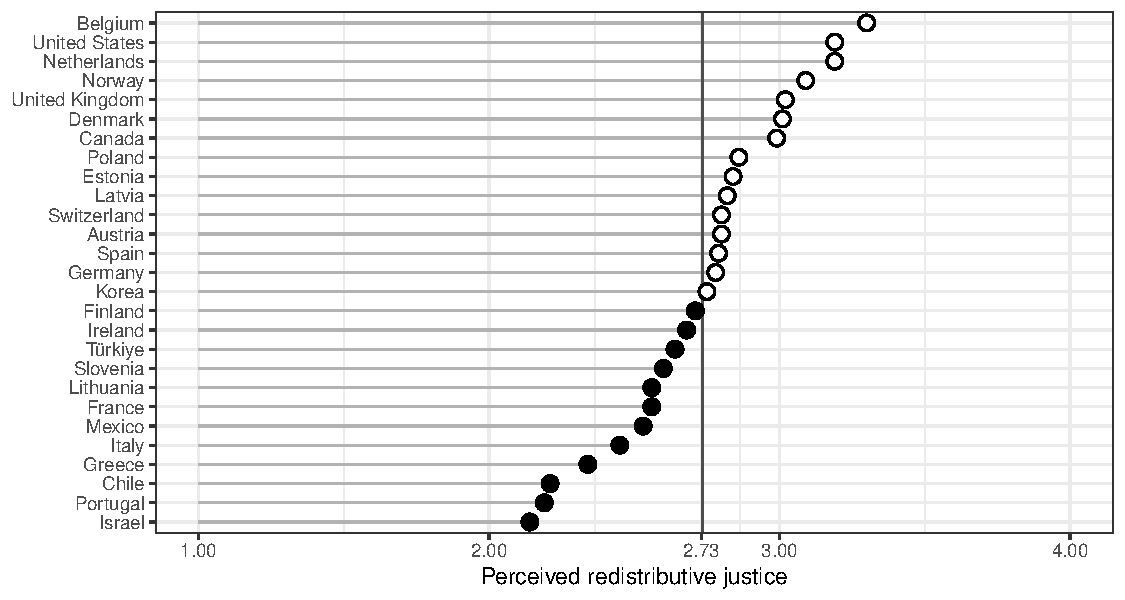
\includegraphics[width=0.85\linewidth,height=\textheight,keepaspectratio]{paper-anonymized_files/figure-pdf/fig-cleveland-1.pdf}

}

\subcaption{\label{fig-cleveland}Source: own elaboration with data from
the OECD, Risks That Matter survey 2024. Perceived redistributive
justice corresponds to the degree of agreement with the item on
receiving a fair share of public benefits given the taxes and
contributions paid (scale 1--5). The vertical grey line shows the OECD
mean of redistributive justice.}

}

\end{figure}%

\subsection{Work, type of employment and platform
economy}\label{work-type-of-employment-and-platform-economy}

The sociology of work has documented in multiple contexts the growing
polarisation between formal, well-paid employment and an expanding
stratum of precarious work (\citeproc{ref-gallie_economic_2013}{Gallie,
2013}; \citeproc{ref-kalleberg_good_2011}{Kalleberg, 2011}). Precarious
work ---uncertain and unpredictable employment that shifts risk from
employers to workers--- has spread beyond the margins of the labour
market to reach growing portions of the workforce
(\citeproc{ref-kalleberg_good_2011}{Kalleberg, 2011}), and is not
reduced to income insecurity, but entails the absence of the
occupational identity, social rights and temporal stability that
characterised the standard employment relationship
(\citeproc{ref-standing_precariat_2014}{Standing, 2014}). These
transformations matter for the welfare state because its institutions
were designed around that formal relationship, so that those who depart
from it tend to maintain a weaker and more unequal link with the
protection system (\citeproc{ref-emmenegger_age_2012}{Emmenegger et al.,
2012}; \citeproc{ref-schwander_who_2013}{Schwander and Häusermann,
2013}). This structural position in the labour market shapes that
material link, and also conditions attitudes towards inequality and
redistribution (\citeproc{ref-lindh_class_2020}{Lindh and McCall,
2020}), an effect especially visible in contexts of marked
commodification such as the Chilean one
(\citeproc{ref-perez-ahumada_conditioning_2026}{Pérez-Ahumada et al.,
2026}).

Type of employment structures that relationship directly. Workers in
formal waged employment contribute through registered contributions and
accumulate rights in a legible way, which makes the relationship between
what they contribute and what they receive traceable. Workers in
non-formal employment face a more opaque and often less favourable
relationship, since the self-employed tend to pay higher net
contributions and remain excluded from unemployment insurance, while
temporary workers accumulate interrupted contribution records that
reduce their future benefits (\citeproc{ref-marx_effect_2014}{Marx,
2014}; \citeproc{ref-rueda_social_2007}{Rueda, 2007}). This
institutional distance between insiders and outsiders in the labour
market creates conditions for the latter to perceive that the system was
not designed for people in their situation, which may translate into a
less favourable assessment of the justice of the fiscal exchange
(\citeproc{ref-schwander_who_2013}{Schwander and Häusermann, 2013}).

Platform-mediated work constitutes a particularly acute form of
non-formal employment. Algorithmic intermediation, the classification of
workers as independent contractors and the fragmentation of tasks place
these workers largely outside the formal architecture of social
insurance (\citeproc{ref-vallas_what_2020}{Vallas and Schor, 2020};
\citeproc{ref-wood_good_2019}{Wood et al., 2019}). Several studies have
shown that platform workers combine nominal autonomy with a high degree
of external control and a fragmented or non-existent social protection
(\citeproc{ref-behrendt_social_2019}{Behrendt et al., 2019};
\citeproc{ref-schor_gig_2020}{Schor, 2020}), a pattern that evidence for
Latin America has documented in platform-mediated delivery, where
classification as independent contractors shifts risk onto workers and
leaves them outside social security
(\citeproc{ref-gutierrezcrocco_effects_2022}{Gutiérrez Crocco and
Atzeni, 2022}). The European directive on platform work responds to this
situation by introducing a legal presumption of employment and rules on
algorithmic management
(\citeproc{ref-europeanparliamentandcounciloftheeuropeanunion_directive_2024}{European
Parliament and Council of the European Union, 2024}). This structural
position exposes these workers to a lack of protection that leads one to
expect a comparatively lower perception of the justice of their
relationship with the welfare state. These considerations give rise to
the first hypothesis:

\begin{tcolorbox}[enhanced jigsaw, arc=.35mm, bottomrule=.15mm, breakable, colback=white, colframe=quarto-callout-color-frame, left=2mm, leftrule=.75mm, opacityback=0, rightrule=.15mm, toprule=.15mm]

H1: Workers in non-formal employment ---platform work and
self-employment--- will perceive lower redistributive justice than
workers in formal waged employment.

\end{tcolorbox}

\subsection{Job insecurity}\label{job-insecurity}

Beyond type of employment, the level of job insecurity experienced by
workers constitutes a distinct dimension of vulnerability. Job
insecurity is defined as the subjective assessment of the concern of
losing one's own job or self-employment income in the short term, with
the chronic uncertainty and anticipatory anxiety this entails
(\citeproc{ref-dewitte_job_2005}{De Witte, 2005};
\citeproc{ref-sverke_no_2002}{Sverke et al., 2002}). Unlike objective
precarity, it is a perceived state that can also affect formally
protected workers and whose effects on behaviour and attitudes are
widely documented (\citeproc{ref-anderson_workers_2007}{Anderson and
Pontusson, 2007}; \citeproc{ref-chung_institutions_2011}{Chung and Van
Oorschot, 2011}).

From the perspective of redistributive justice, job insecurity raises
what is at stake in the relationship between contributions and benefits.
The literature on risk and redistribution has shown that exposure to
insecurity increases support for social protection
(\citeproc{ref-cusack_risks_2006}{Cusack et al., 2006};
\citeproc{ref-iversen_asset_2001}{Iversen and Soskice, 2001};
\citeproc{ref-rehm_risks_2009}{Rehm, 2009}). The relationship with
perceived redistributive justice may, however, operate in a different
direction: workers who anticipate losing their job assess with greater
scrutiny what they would receive from the state in that scenario, and
when that expectation is not accompanied by confidence in the protective
capacity of the system, they are likely to perceive the exchange as less
just (\citeproc{ref-marx_effect_2014}{Marx, 2014}). The second
hypothesis is thus proposed:

\begin{tcolorbox}[enhanced jigsaw, arc=.35mm, bottomrule=.15mm, breakable, colback=white, colframe=quarto-callout-color-frame, left=2mm, leftrule=.75mm, opacityback=0, rightrule=.15mm, toprule=.15mm]

H2: Greater perceived job insecurity will be associated with a lower
perception of redistributive justice.

\end{tcolorbox}

\subsection{Perceived technological
change}\label{perceived-technological-change}

The rise of digital technologies has introduced an additional source of
occupational vulnerability, distinct from conventional job insecurity.
Estimates of the proportion of jobs susceptible to automation vary
widely, but even the most conservative ones anticipate significant
changes in the content of tasks and in the viability of numerous
occupations (\citeproc{ref-arntz_risk_2016}{Arntz et al., 2016};
\citeproc{ref-autor_why_2015}{Autor, 2015};
\citeproc{ref-bustelo_automation_2020}{Bustelo et al., 2020};
\citeproc{ref-frey_future_2017}{Frey and Osborne, 2017}). What matters
for welfare attitudes is the objective magnitude of that process, and
also the way in which workers anticipate its effects on their own job
(\citeproc{ref-gallego_automation_2022}{Gallego and Kurer, 2022}). That
anticipation comprises both the perception of a displacement risk (the
probability of losing the job to technology) and the perception of a
benefit (the probability that technology will improve the quality of
work).

\subsubsection{Perception of technological displacement
risk}\label{perception-of-technological-displacement-risk}

On the one hand, technological change refers to the perception of
technological displacement risk, that is, the probability that one's own
job will be replaced by a robot or by artificial intelligence,
substituted by a provider offering a similar service through a platform,
or rendered unviable by the obsolescence of one's own digital skills.
Research has shown that the fear of automation is distributed unevenly
across occupations and social groups and that it has measurable
political and attitudinal consequences
(\citeproc{ref-dekker_fear_2017}{Dekker et al., 2017};
\citeproc{ref-im_losers_2019}{Im et al., 2019};
\citeproc{ref-kurer_declining_2020}{Kurer, 2020}). The literature on
risk and redistribution has robustly established that perceived exposure
to technological risk increases the demand for social protection
(\citeproc{ref-busemeyer_social_2022}{Busemeyer and Sahm, 2022};
\citeproc{ref-iversen_asset_2001}{Iversen and Soskice, 2001};
\citeproc{ref-rehm_risks_2009}{Rehm, 2009};
\citeproc{ref-thewissen_automation_2019}{Thewissen and Rueda, 2019}).
Following that logic, workers who perceive their job as threatened by
technology hold greater expectations of protection and, when contrasting
these with what they actually receive, are more likely to assess their
exchange with the welfare state as insufficient
(\citeproc{ref-marx_effect_2014}{Marx, 2014}). The third hypothesis is
thus derived:

\begin{tcolorbox}[enhanced jigsaw, arc=.35mm, bottomrule=.15mm, breakable, colback=white, colframe=quarto-callout-color-frame, left=2mm, leftrule=.75mm, opacityback=0, rightrule=.15mm, toprule=.15mm]

H3: Workers who perceive a higher probability of being displaced by
automation, platform competition or the obsolescence of their skills
will report a lower perception of redistributive justice.

\end{tcolorbox}

\subsubsection{Perception of technological
benefit}\label{perception-of-technological-benefit}

On the other hand, technological change refers to the perception of
technological benefit, which addresses the probability that technology
will make working hours more compatible with private life, reduce the
dangerousness or physical demands of work, or lessen its monotony and
mental load. This enabling dimension has received much less attention
than its threatening counterpart, even though workers' orientation
towards technology is not solely negative
(\citeproc{ref-autor_why_2015}{Autor, 2015};
\citeproc{ref-brougham_smart_2018}{Brougham and Haar, 2018}). Unlike
displacement risk, perceiving technology as an improvement in working
conditions implies lower exposure to risk and greater optimism about
one's occupational trajectory. To the extent that the assessment of the
exchange with the welfare state reflects the individual's position of
economic security (\citeproc{ref-rehm_risks_2009}{Rehm, 2009}), this
positive orientation can be expected to be associated with a more
favourable perception of redistributive justice. The fourth hypothesis
follows from this:

\begin{tcolorbox}[enhanced jigsaw, arc=.35mm, bottomrule=.15mm, breakable, colback=white, colframe=quarto-callout-color-frame, left=2mm, leftrule=.75mm, opacityback=0, rightrule=.15mm, toprule=.15mm]

H4: Workers who perceive technology as enabling ---reducing physical
demands, improving the balance between work and private life or making
work less stressful or monotonous--- will perceive greater
redistributive justice.

\end{tcolorbox}

\subsection{Perceived deservingness of
others}\label{perceived-deservingness-of-others}

Perceptions of redistributive justice do not depend solely on structural
position, but also on the normative frameworks through which individuals
assess who and what deserves to receive from the state. Deservingness
literature holds that people direct their solidarity towards the groups
they consider deserving and withdraw it from those they judge
undeserving, on the basis of criteria such as control over one's own
situation, attitude, reciprocity, identity and need
(\citeproc{ref-petersen_social_2012}{Petersen, 2012};
\citeproc{ref-oorschot_who_2000}{Van Oorschot, 2000}). In strongly
commodified contexts, meritocratic and market-justice beliefs reinforce
the tendency to consider undeserving those who are perceived not to
contribute enough (\citeproc{ref-castillo_perceptions_2025}{Castillo et
al., 2025}). These judgements about the deservingness of others are
analytically distinct from the judgement about the justice of one's own
relationship with the system: a person may consider themselves a
contributor who does not receive their just share and, at the same time,
judge that others receive benefits they do not deserve. Both assessments
are, however, part of the same moral economy of welfare, and they can be
expected to be connected (\citeproc{ref-mau_moral_2014}{Mau, 2014};
\citeproc{ref-vanoorschot_social_2017}{Van Oorschot et al., 2017}).

The connection between the two judgements operates through the norm of
reciprocity. The resources that an individual contributes appear to
sustain those who do not fulfil their part, which erodes the sense that
the system treats them in a just way
(\citeproc{ref-cavaille_fair_2025}{Cavaillé, 2025};
\citeproc{ref-reeskens_equity_2013}{Reeskens and Van Oorschot, 2013}).
Comparative research has shown that deservingness perceptions robustly
structure support for the welfare state and that the control criterion
occupies a central place in those judgements
(\citeproc{ref-laenen_welfare_2020}{Laenen, 2020};
\citeproc{ref-vanoorschot_making_2006}{Van Oorschot, 2006}). It can
therefore be expected that those who perceive greater abuse of the
system by others will assess their own relationship with it as less
just. The fifth hypothesis is proposed:

\begin{tcolorbox}[enhanced jigsaw, arc=.35mm, bottomrule=.15mm, breakable, colback=white, colframe=quarto-callout-color-frame, left=2mm, leftrule=.75mm, opacityback=0, rightrule=.15mm, toprule=.15mm]

H5: Workers who perceive that many people receive public benefits
without deserving them will report a lower perception of redistributive
justice.

\end{tcolorbox}

\subsection{Welfare regimes and institutional
context}\label{welfare-regimes-and-institutional-context}

Individual perceptions of redistributive justice are formed in
institutional contexts that vary systematically across welfare regimes
(\citeproc{ref-arts_three_2002}{Arts and Gelissen, 2002};
\citeproc{ref-esping-andersen_three_1993}{Esping-Andersen, 1990}). The
classic typology of Esping-Andersen
(\citeproc{ref-esping-andersen_three_1993}{1990}) distinguishes three
worlds of welfare capitalism according to how they organise the
relationship between state, market and family in the provision of social
protection. In social democratic regimes (mainly Nordic countries),
protection is comprehensive and universal, and redistribution
constitutes a central expression of social solidarity sustained by
universalist institutions (\citeproc{ref-korpi_paradox_1998}{Korpi and
Palme, 1998}). In liberal regimes (mainly Anglo-Saxon countries and, for
example, Chile as a case of a commodified welfare state in Latin
America), protection is residual and targeted, is organised around
market participation and is politically more contested
(\citeproc{ref-franzoni_welfare_2008}{Martínez Franzoni, 2008};
\citeproc{ref-perez_building_2023}{Pérez-Ahumada, 2023}). In
conservative-corporatist regimes (continental Europe), rights are
strongly tied to employment status, which preserves status differences
and links protection to the employment trajectory
(\citeproc{ref-ferrera_southern_1996}{Ferrera, 1996}).

Alongside institutional design, macroeconomic factors bear on welfare
attitudes: income inequality is associated with perceptions of the
justice of the system, although the direction of that relationship is a
matter of debate (\citeproc{ref-finseraas_income_2009}{Finseraas, 2009};
\citeproc{ref-schmidt-catran_economic_2016}{Schmidt-Catran, 2016}), and
the level of economic development conditions both the fiscal capacity of
the state and citizens' expectations regarding social protection
(\citeproc{ref-blekesaune_public_2003}{Blekesaune, 2003}). Taken
together, the perception of redistributive justice can be expected to
be, on average, higher in social democratic regimes, where protection is
more comprehensive and universal, than in liberal and conservative
regimes (\citeproc{ref-jaeger_welfare_2006}{Jæger, 2006};
\citeproc{ref-larsen_institutional_2008}{Larsen, 2008};
\citeproc{ref-svallfors_worlds_1997}{Svallfors, 1997}). Hence the sixth
hypothesis:

\begin{tcolorbox}[enhanced jigsaw, arc=.35mm, bottomrule=.15mm, breakable, colback=white, colframe=quarto-callout-color-frame, left=2mm, leftrule=.75mm, opacityback=0, rightrule=.15mm, toprule=.15mm]

H6: On average, workers in social democratic regimes will perceive
higher redistributive justice than workers in liberal and conservative
regimes.

\end{tcolorbox}

The institutional context shifts the average level of perceptions, and
may moderate the effect of individual predictors. The institutional
distance between workers in non-formal employment and the protection
system is greater in liberal and conservative regimes than in social
democratic ones, which are universalist in character
(\citeproc{ref-ferrera_southern_1996}{Ferrera, 1996};
\citeproc{ref-schwander_who_2013}{Schwander and Häusermann, 2013}). It
can therefore be expected that the negative effect of labour market
position on perceived redistributive justice will be more pronounced in
the former:

\begin{tcolorbox}[enhanced jigsaw, arc=.35mm, bottomrule=.15mm, breakable, colback=white, colframe=quarto-callout-color-frame, left=2mm, leftrule=.75mm, opacityback=0, rightrule=.15mm, toprule=.15mm]

H7: The negative relationship between non-standard employment (platform
work and self-employment) and perceived redistributive justice will be
moderated by the welfare regime.

\end{tcolorbox}

An analogous expectation can be formulated for the perception of
technological risk. In universalist regimes, protection against the
risks associated with digitalisation is more robust and less dependent
on the individual employment trajectory, which could moderate the effect
of perceived displacement risk on the assessment of the fiscal exchange
(\citeproc{ref-busemeyer_social_2022}{Busemeyer and Sahm, 2022};
\citeproc{ref-fan_how_2024}{Fan et al., 2024};
\citeproc{ref-gallego_automation_2022}{Gallego and Kurer, 2022}):

\begin{tcolorbox}[enhanced jigsaw, arc=.35mm, bottomrule=.15mm, breakable, colback=white, colframe=quarto-callout-color-frame, left=2mm, leftrule=.75mm, opacityback=0, rightrule=.15mm, toprule=.15mm]

H8: The negative effect of the perception of technological displacement
risk on the perception of redistributive justice will be moderated by
the welfare regime.

\end{tcolorbox}

Finally, the salience of deservingness judgements varies according to
institutional design. In universalist regimes, where benefits are
conceived as general rights rather than as targeted assistance, the
distinctions between deserving and undeserving tend to be less
pronounced than in residual regimes, organised around means testing
(\citeproc{ref-larsen_institutional_2008}{Larsen, 2008};
\citeproc{ref-vanoorschot_social_2017}{Van Oorschot et al., 2017}). It
can therefore be expected that the effect of the perceived deservingness
of others on the justice of one's own exchange will be stronger in
liberal and conservative regimes:

\begin{tcolorbox}[enhanced jigsaw, arc=.35mm, bottomrule=.15mm, breakable, colback=white, colframe=quarto-callout-color-frame, left=2mm, leftrule=.75mm, opacityback=0, rightrule=.15mm, toprule=.15mm]

H9: The negative effect of the perceived deservingness of others on the
perception of redistributive justice will be moderated by the welfare
regime.

\end{tcolorbox}

\section{Data, variables and methods}\label{data-variables-and-methods}

\subsection{Data}\label{data}

This study uses data from the most recent wave (2024) of the Risks That
Matter (RTM) survey of the OECD (\citeproc{ref-oecd_risks_2024}{OECD,
2024}), a cross-national public opinion survey covering 27,229 people
aged 18 to 64 in 27 member countries (Austria, Belgium, Canada, Chile,
Denmark, Estonia, Finland, France, Germany, Greece, Ireland, Israel,
Italy, Korea, Latvia, Lithuania, Mexico, the Netherlands, Norway,
Poland, Portugal, Slovenia, Spain, Switzerland, Türkiye, the United
Kingdom and the United States). The survey is fielded online and
weighted with post-stratification weights calibrated by age, sex, region
and educational level (\citeproc{ref-thomas_survey_2025}{Thomas et al.,
2025}). The 2024 wave captures attitudes in the period after the
COVID-19 pandemic, which accelerated the digitalisation of work and
expanded platform employment.

The analysis is restricted to respondents who were in paid work in the
week before the interview or temporarily away from a job for health or
other reasons (n = 22,063). This restriction follows the structure of
the questionnaire. The items on type of employment, platform work and
perceived technological change refer to the respondent's own job and are
only administered to those attached to the labour market, so the 5,166
respondents who were not employed, whether seeking work or not, do not
enter the analysis by design. After listwise deletion of cases with
missing values on the model variables, the final analytic sample
comprises 19,669 respondents, 89.1 per cent of the eligible sample.
Sample sizes by country are reported in the appendix at
Table~\ref{tbl-classification}.

\subsection{Variables}\label{variables}

The dependent variable is the perception of redistributive justice,
measured by the item ``I feel that I receive a fair share of public
benefits, given the taxes and social contributions that I pay and/or
have paid in the past''. Responses are recorded on a five-point Likert
scale from strongly disagree to strongly agree, and the variable is
treated as ordinal in all the analyses.

Three sets of independent variables constitute the core of the analysis.
The first concerns labour market position and job insecurity. Labour
market position is captured by two binary indicators, one identifying
self-employed workers and one identifying platform workers, understood
as those whose work is mediated by digital platforms. The two indicators
are not mutually exclusive, since platform work is often carried out
under self-employment arrangements. Respondents scoring zero on both
correspond to formal dependent employment, which serves as the reference
situation, and the overlap between the two categories is examined
directly in the analysis. Job insecurity is measured by the item
``Losing a job or self-employment income'', asked within the battery
``Thinking about the next year or two, how concerned are you about each
of the following?'', with response categories from not at all concerned
to very concerned.

The second set captures the perception of technological change with
respect to one's own job, measured through the battery ``How likely do
you think it is that the following will happen in your job (or job
opportunities) in the next five years?'', with items rated on a
four-point probability scale. Four items refer to displacement. They ask
about the replacement of the job by a robot, by an artificial
intelligence tool such as ChatGPT, or by a person offering a similar
service through an internet platform, and about losing the job through
not being sufficiently technologically skilled. Three items refer to
benefits. They ask whether technology will make working hours more
compatible with private life, make work less dangerous or physically
demanding, and make it less boring, repetitive, stressful or mentally
demanding. An exploratory factor analysis of the seven items supports a
two-factor structure. Three of the four displacement items load on a
first factor and the three benefit items on a second, while the item on
replacement by artificial intelligence defines a separate third
dimension suggested by the parallel analysis and is excluded from the
scales.\footnote{As a robustness check, the models were re-estimated
  including this item as an additional predictor. Its coefficient was
  not significant and the remaining estimates were substantively
  unchanged.} Two scales are built accordingly, Technological
Displacement Risk (the average of the three displacement items) and
Perceived Technological Benefit (the average of the three benefit
items). In both cases higher values indicate a stronger perception of
the corresponding risk or benefit. The full factor analysis is reported
in the appendix at Table~\ref{tbl-efa}.

The third set concerns the perceived deservingness of others,
operationalised through the degree of agreement with the statement
``Many people receive public benefits without deserving them'', rated on
a five-point scale (1 = strongly disagree to 5 = strongly agree). This
item refers to the deservingness of other beneficiaries, while the
dependent variable refers to the respondent's own exchange with the
system, a distinction that is central in the deservingness literature
(\citeproc{ref-oorschot_who_2000}{Van Oorschot, 2000},
\citeproc{ref-vanoorschot_making_2006}{2006}). Higher values indicate a
stronger perception that others receive benefits without deserving them.

The welfare regime is operationalised as a three-category variable that
distinguishes social democratic, liberal and conservative-corporatist
regimes, following Esping-Andersen
(\citeproc{ref-esping-andersen_three_1993}{1990}) and Bambra
(\citeproc{ref-bambra_sifting_2007}{2007}). The countries of southern
Europe and of central and eastern Europe are integrated into the
conservative category, given the initial specificity of the
post-socialist regimes and their progressive convergence towards the
continental types (\citeproc{ref-Fenger2006WelfareRI}{Fenger, 2006};
\citeproc{ref-ferrera_southern_1996}{Ferrera, 1996}), while the Baltic
states, characterised by a more liberal orientation of their
post-socialist reforms, are incorporated into the liberal regime
(\citeproc{ref-aidukaite_welfare_2011}{Aidukaite, 2011}). Among the
non-European countries, Chile and Mexico are classified as liberal,
following the characterisation of their welfare regimes as
market-centred (\citeproc{ref-franzoni_welfare_2008}{Martínez Franzoni,
2008}), while Israel, Korea and Türkiye are assigned to the conservative
category. The full classification by country, with its sources, is
reported in the appendix at Table~\ref{tbl-classification}.

At the country level the models include four macroeconomic indicators.
The Gini coefficient of disposable income, GDP per capita (PPP, constant
international dollars) and the unemployment rate (ILO estimate) are
drawn from the World Bank's World Development Indicators, and public
social expenditure as a percentage of GDP is drawn from the OECD Social
Expenditure Database (SOCX). For each country the most recent value
available within the 2015--2024 window is used. GDP per capita is
log-transformed, and all four indicators are grand-mean standardised, so
that their coefficients express the association with a difference of one
standard deviation between countries. Income inequality and the level of
economic development have been shown to condition welfare attitudes
(\citeproc{ref-blekesaune_public_2003}{Blekesaune, 2003};
\citeproc{ref-finseraas_income_2009}{Finseraas, 2009};
\citeproc{ref-schmidt-catran_economic_2016}{Schmidt-Catran, 2016}),
while social expenditure provides a continuous indicator of welfare
effort that complements the categorical regime typology.

All the models include sex, age, educational level (highest level of
studies completed) and income decile (self-reported position in the
national income distribution) as control variables associated with
welfare attitudes and perceived redistributive justice.

A summary of these variables and their main descriptive statistics is
available in Table~\ref{tbl-summary}; the macroeconomic indicators are
reported there on their original scales, with statistics computed over
individuals, so each country contributes in proportion to its sample
size.

\begin{longtable}[]{@{}
  >{\raggedright\arraybackslash}p{(\linewidth - 6\tabcolsep) * \real{0.3925}}
  >{\raggedright\arraybackslash}p{(\linewidth - 6\tabcolsep) * \real{0.3084}}
  >{\raggedright\arraybackslash}p{(\linewidth - 6\tabcolsep) * \real{0.1963}}
  >{\raggedright\arraybackslash}p{(\linewidth - 6\tabcolsep) * \real{0.1028}}@{}}
\caption{Main descriptive statistics}\label{tbl-summary}\tabularnewline
\toprule\noalign{}
\begin{minipage}[b]{\linewidth}\raggedright
Label
\end{minipage} & \begin{minipage}[b]{\linewidth}\raggedright
Stats / Values
\end{minipage} & \begin{minipage}[b]{\linewidth}\raggedright
Freqs (\% of Valid)
\end{minipage} & \begin{minipage}[b]{\linewidth}\raggedright
Valid
\end{minipage} \\
\midrule\noalign{}
\endfirsthead
\toprule\noalign{}
\begin{minipage}[b]{\linewidth}\raggedright
Label
\end{minipage} & \begin{minipage}[b]{\linewidth}\raggedright
Stats / Values
\end{minipage} & \begin{minipage}[b]{\linewidth}\raggedright
Freqs (\% of Valid)
\end{minipage} & \begin{minipage}[b]{\linewidth}\raggedright
Valid
\end{minipage} \\
\midrule\noalign{}
\endhead
\bottomrule\noalign{}
\endlastfoot
Redistributive justice & \begin{minipage}[t]{\linewidth}\raggedright
1. Strongly disagree\\
2. Disagree\\
3. Neither agree nor disagre\\
4. Agree\\
5. Strongly agree\strut
\end{minipage} & \begin{minipage}[t]{\linewidth}\raggedright
3600 (18.3\%)\\
4765 (24.2\%)\\
5641 (28.7\%)\\
4255 (21.6\%)\\
1408 ( 7.2\%)\strut
\end{minipage} & \begin{minipage}[t]{\linewidth}\raggedright
19669\\
(100.0\%)\strut
\end{minipage} \\
Sex & \begin{minipage}[t]{\linewidth}\raggedright
1. Man\\
2. Woman\strut
\end{minipage} & \begin{minipage}[t]{\linewidth}\raggedright
10520 (53.5\%)\\
9149 (46.5\%)\strut
\end{minipage} & \begin{minipage}[t]{\linewidth}\raggedright
19669\\
(100.0\%)\strut
\end{minipage} \\
Age group & \begin{minipage}[t]{\linewidth}\raggedright
1. 18-24\\
2. 25-34\\
3. 35-44\\
4. 45-54\\
5. 55-64\strut
\end{minipage} & \begin{minipage}[t]{\linewidth}\raggedright
2136 (10.9\%)\\
4626 (23.5\%)\\
4854 (24.7\%)\\
4599 (23.4\%)\\
3454 (17.6\%)\strut
\end{minipage} & \begin{minipage}[t]{\linewidth}\raggedright
19669\\
(100.0\%)\strut
\end{minipage} \\
Educational level & \begin{minipage}[t]{\linewidth}\raggedright
1. Low\\
2. Medium\\
3. High\strut
\end{minipage} & \begin{minipage}[t]{\linewidth}\raggedright
1546 ( 7.9\%)\\
8147 (41.4\%)\\
9976 (50.7\%)\strut
\end{minipage} & \begin{minipage}[t]{\linewidth}\raggedright
19669\\
(100.0\%)\strut
\end{minipage} \\
Equivalised disposable household income decile (2023) &
\begin{minipage}[t]{\linewidth}\raggedright
Mean (sd) : 4.9 (2.9)\\
min \textless{} med \textless{} max:\\
1 \textless{} 5 \textless{} 10\\
IQR (CV) : 5 (0.6)\strut
\end{minipage} & \begin{minipage}[t]{\linewidth}\raggedright
1 : 3398 (17.3\%)\\
2 : 1844 ( 9.4\%)\\
3 : 1788 ( 9.1\%)\\
4 : 2652 (13.5\%)\\
5 : 2322 (11.8\%)\\
6 : 1815 ( 9.2\%)\\
7 : 1488 ( 7.6\%)\\
8 : 1424 ( 7.2\%)\\
9 : 1300 ( 6.6\%)\\
10 : 1638 ( 8.3\%)\strut
\end{minipage} & \begin{minipage}[t]{\linewidth}\raggedright
19669\\
(100.0\%)\strut
\end{minipage} \\
Self-employment worker & \begin{minipage}[t]{\linewidth}\raggedright
1. No\\
2. Yes\strut
\end{minipage} & \begin{minipage}[t]{\linewidth}\raggedright
16887 (85.9\%)\\
2782 (14.1\%)\strut
\end{minipage} & \begin{minipage}[t]{\linewidth}\raggedright
19669\\
(100.0\%)\strut
\end{minipage} \\
Platform worker & \begin{minipage}[t]{\linewidth}\raggedright
1. No\\
2. Yes\strut
\end{minipage} & \begin{minipage}[t]{\linewidth}\raggedright
17825 (90.6\%)\\
1844 ( 9.4\%)\strut
\end{minipage} & \begin{minipage}[t]{\linewidth}\raggedright
19669\\
(100.0\%)\strut
\end{minipage} \\
Lose job & \begin{minipage}[t]{\linewidth}\raggedright
1. Not at all concerned\\
2. Not so concerned\\
3. Somewhat concerned\\
4. Very concerned\strut
\end{minipage} & \begin{minipage}[t]{\linewidth}\raggedright
2927 (14.9\%)\\
5453 (27.7\%)\\
6110 (31.1\%)\\
5179 (26.3\%)\strut
\end{minipage} & \begin{minipage}[t]{\linewidth}\raggedright
19669\\
(100.0\%)\strut
\end{minipage} \\
Technological displacement & \begin{minipage}[t]{\linewidth}\raggedright
Mean (sd) : 2.1 (0.9)\\
min \textless{} med \textless{} max:\\
1 \textless{} 2 \textless{} 4\\
IQR (CV) : 1.3 (0.4)\strut
\end{minipage} & 13 distinct values &
\begin{minipage}[t]{\linewidth}\raggedright
19669\\
(100.0\%)\strut
\end{minipage} \\
Perceived technological benefit &
\begin{minipage}[t]{\linewidth}\raggedright
Mean (sd) : 2.6 (0.8)\\
min \textless{} med \textless{} max:\\
1 \textless{} 2.7 \textless{} 4\\
IQR (CV) : 1 (0.3)\strut
\end{minipage} & 13 distinct values &
\begin{minipage}[t]{\linewidth}\raggedright
19669\\
(100.0\%)\strut
\end{minipage} \\
Deservingness of others & \begin{minipage}[t]{\linewidth}\raggedright
1. Strongly disagree\\
2. Disagree\\
3. Neither agree nor disagre\\
4. Agree\\
5. Strongly agree\strut
\end{minipage} & \begin{minipage}[t]{\linewidth}\raggedright
624 ( 3.2\%)\\
1727 ( 8.8\%)\\
4434 (22.5\%)\\
6670 (33.9\%)\\
6214 (31.6\%)\strut
\end{minipage} & \begin{minipage}[t]{\linewidth}\raggedright
19669\\
(100.0\%)\strut
\end{minipage} \\
Welfare regime & \begin{minipage}[t]{\linewidth}\raggedright
1. Liberal\\
2. Social-democratic\\
3. Conservative\strut
\end{minipage} & \begin{minipage}[t]{\linewidth}\raggedright
6563 (33.4\%)\\
2957 (15.0\%)\\
10149 (51.6\%)\strut
\end{minipage} & \begin{minipage}[t]{\linewidth}\raggedright
19669\\
(100.0\%)\strut
\end{minipage} \\
Gini coefficient (disposable income) &
\begin{minipage}[t]{\linewidth}\raggedright
Mean (sd) : 32.8 (5)\\
min \textless{} med \textless{} max:\\
24.7 \textless{} 32.4 \textless{} 43.7\\
IQR (CV) : 5 (0.2)\strut
\end{minipage} & 26 distinct values &
\begin{minipage}[t]{\linewidth}\raggedright
19669\\
(100.0\%)\strut
\end{minipage} \\
GDP per capita (PPP) & \begin{minipage}[t]{\linewidth}\raggedright
Mean (sd) : 57093.7 (20396.3)\\
min \textless{} med \textless{} max:\\
21970.4 \textless{} 53412.1 \textless{} 118833.3\\
IQR (CV) : 18634.9 (0.4)\strut
\end{minipage} & 27 distinct values &
\begin{minipage}[t]{\linewidth}\raggedright
19669\\
(100.0\%)\strut
\end{minipage} \\
Unemployment rate (\%) & \begin{minipage}[t]{\linewidth}\raggedright
Mean (sd) : 5.7 (2.3)\\
min \textless{} med \textless{} max:\\
2.7 \textless{} 5.2 \textless{} 11.4\\
IQR (CV) : 3.2 (0.4)\strut
\end{minipage} & 25 distinct values &
\begin{minipage}[t]{\linewidth}\raggedright
19669\\
(100.0\%)\strut
\end{minipage} \\
Social expenditure (\% of GDP) &
\begin{minipage}[t]{\linewidth}\raggedright
Mean (sd) : 21.5 (6)\\
min \textless{} med \textless{} max:\\
10 \textless{} 23 \textless{} 31.6\\
IQR (CV) : 10.1 (0.3)\strut
\end{minipage} & 27 distinct values &
\begin{minipage}[t]{\linewidth}\raggedright
19669\\
(100.0\%)\strut
\end{minipage} \\
\end{longtable}

\subsection{Methods}\label{methods}

The hypotheses were pre-registered on the Open Science Framework
(anonymised view-only
\href{https://osf.io/bw26x/overview?view_only=13afa066aea3483f8e970a6a65c1f07a}{link}).
Statistical analyses were conducted in R version 4.3.2, and the models
are estimated with the clmm function of the ordinal package
(\citeproc{ref-haubo_cumulative_2018}{Christensen, 2018}).

Multilevel ordinal logistic regression models with individuals nested in
countries are used to examine the relationship between labour market
position, the perceptions of technological displacement and benefit, the
deservingness of others and perceived redistributive justice. This
approach accounts for the hierarchical structure of the comparative data
and decomposes the variance of the outcome into individual and country
components (\citeproc{ref-hox_multilevel_2017}{Hox et al., 2017};
\citeproc{ref-snijders_multilevel_2012}{Snijders and Bosker, 2012}),
with random intercepts estimated for each country. An unconditional
model without predictors is estimated first to establish the share of
the variance located at the country level.

The models are estimated sequentially. At the individual level, Model 1
enters the two labour market indicators, Model 2 adds job insecurity,
Model 3 the two technological perceptions, Model 4 the perceived
deservingness of others and Model 5 the sociodemographic controls. The
country level is then incorporated, with the macroeconomic indicators in
Models 6 and 7 and the welfare regime in Model 8.

Model 9 introduces the interaction between the two labour market
indicators, and Models 10 to 14 add cross-level interactions between the
welfare regime and each individual-level predictor to test the
moderation hypotheses. All the analyses use the individual survey
weights provided by the OECD. The clmm function treats these as
frequency weights, so the number of observations reported in the tables
corresponds to the sum of the weights (17,296), while the models are
estimated on the 19,669 respondents of the analytic sample.

\section{Analysis}\label{analysis}



Figure~\ref{fig-correlation} presents the correlation matrix of the main
variables, with coefficients ranging from low to moderate. The strongest
associations of perceived redistributive justice are with being a
platform worker (r = 0.32, p \textless{} 0.001), perceived technological
benefit (r = 0.26, p \textless{} 0.001) and technological displacement
(r = 0.24, p \textless{} 0.001), all of them positive and moderate.
Deservingness of others, in contrast, shows a negative association (r =
−0.16, p \textless{} 0.01).

Among the independent variables, concern about job and income loss
correlates with being a platform worker (r = 0.15, p \textless{} 0.001)
and with the two technological perceptions (r = 0.30 with displacement;
r = 0.17 with benefit). Technological displacement and perceived benefit
are themselves positively correlated (r = 0.48), contrary to the initial
intuition that risk and benefit perceptions would be negatively related.

\begin{figure}

\caption{\label{fig-correlation}Correlation matrix of the main
variables}

\centering{

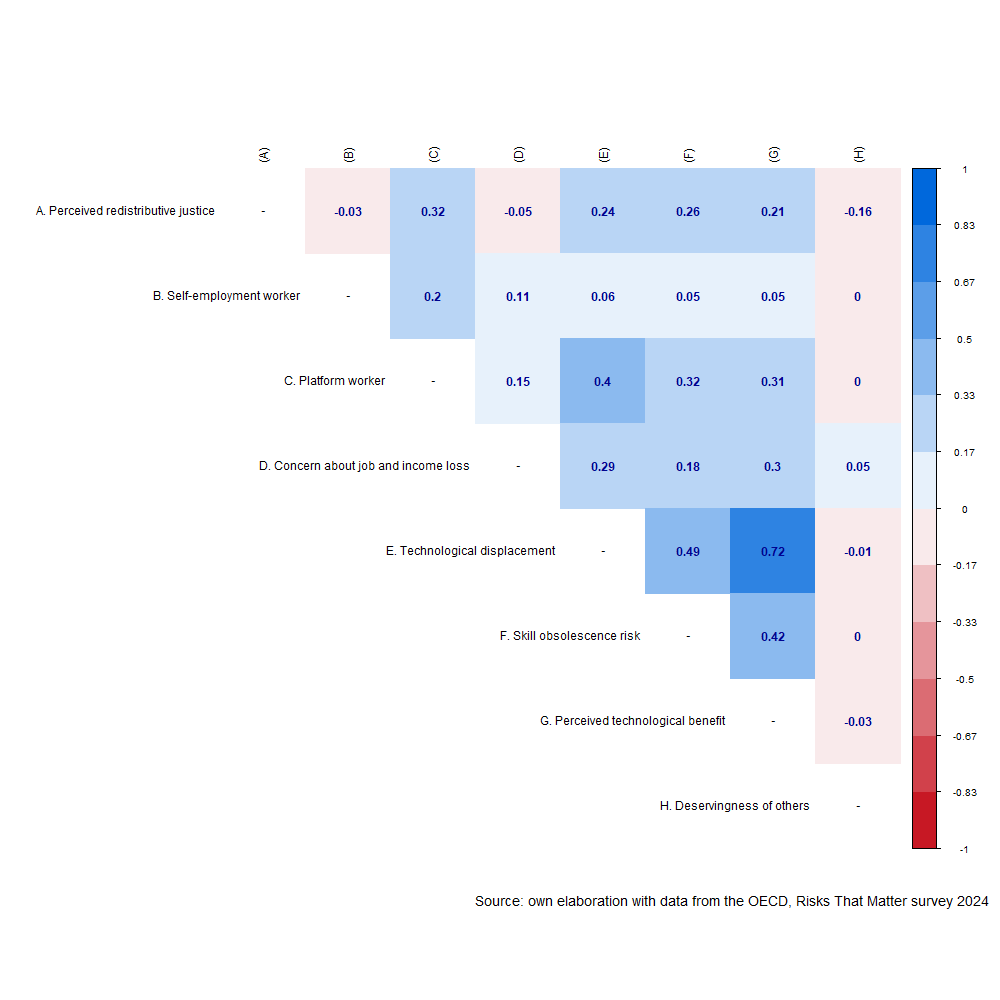
\includegraphics[width=0.85\linewidth,height=\textheight,keepaspectratio]{output/figures/corrplot.png}

}

\end{figure}%

\subsection{Multilevel ordinal logistic regression
models}\label{multilevel-ordinal-logistic-regression-models}

\global\setlength{\Oldarrayrulewidth}{\arrayrulewidth}

\global\setlength{\Oldtabcolsep}{\tabcolsep}

\setlength{\tabcolsep}{2pt}

\renewcommand*{\arraystretch}{1.5}



\providecommand{\ascline}[3]{\noalign{\global\arrayrulewidth #1}\arrayrulecolor[HTML]{#2}\cline{#3}}

\begin{longtable}[c]{|p{1.57in}|p{0.63in}|p{0.63in}|p{0.63in}|p{0.63in}|p{0.63in}|p{0.63in}|p{0.63in}|p{0.63in}}

\caption{\label{tbl-modelos}Multilevel models for perceived
redistributive justice}

\tabularnewline

\ascline{1.5pt}{666666}{1-9}

\multicolumn{1}{>{\raggedright}m{\dimexpr 1.57in+0\tabcolsep}}{\textcolor[HTML]{000000}{\fontsize{8}{7}\selectfont{\textbf{}}}} & \multicolumn{1}{>{\centering}m{\dimexpr 0.63in+0\tabcolsep}}{\textcolor[HTML]{000000}{\fontsize{8}{7}\selectfont{\textbf{Model\ 1}}}} & \multicolumn{1}{>{\centering}m{\dimexpr 0.63in+0\tabcolsep}}{\textcolor[HTML]{000000}{\fontsize{8}{7}\selectfont{\textbf{Model\ 2}}}} & \multicolumn{1}{>{\centering}m{\dimexpr 0.63in+0\tabcolsep}}{\textcolor[HTML]{000000}{\fontsize{8}{7}\selectfont{\textbf{Model\ 3}}}} & \multicolumn{1}{>{\centering}m{\dimexpr 0.63in+0\tabcolsep}}{\textcolor[HTML]{000000}{\fontsize{8}{7}\selectfont{\textbf{Model\ 4}}}} & \multicolumn{1}{>{\centering}m{\dimexpr 0.63in+0\tabcolsep}}{\textcolor[HTML]{000000}{\fontsize{8}{7}\selectfont{\textbf{Model\ 5}}}} & \multicolumn{1}{>{\centering}m{\dimexpr 0.63in+0\tabcolsep}}{\textcolor[HTML]{000000}{\fontsize{8}{7}\selectfont{\textbf{Model\ 6}}}} & \multicolumn{1}{>{\centering}m{\dimexpr 0.63in+0\tabcolsep}}{\textcolor[HTML]{000000}{\fontsize{8}{7}\selectfont{\textbf{Model\ 7}}}} & \multicolumn{1}{>{\centering}m{\dimexpr 0.63in+0\tabcolsep}}{\textcolor[HTML]{000000}{\fontsize{8}{7}\selectfont{\textbf{Model\ 8}}}} \\

\ascline{1.5pt}{666666}{1-9}\endfirsthead 

\ascline{1.5pt}{666666}{1-9}

\multicolumn{1}{>{\raggedright}m{\dimexpr 1.57in+0\tabcolsep}}{\textcolor[HTML]{000000}{\fontsize{8}{7}\selectfont{\textbf{}}}} & \multicolumn{1}{>{\centering}m{\dimexpr 0.63in+0\tabcolsep}}{\textcolor[HTML]{000000}{\fontsize{8}{7}\selectfont{\textbf{Model\ 1}}}} & \multicolumn{1}{>{\centering}m{\dimexpr 0.63in+0\tabcolsep}}{\textcolor[HTML]{000000}{\fontsize{8}{7}\selectfont{\textbf{Model\ 2}}}} & \multicolumn{1}{>{\centering}m{\dimexpr 0.63in+0\tabcolsep}}{\textcolor[HTML]{000000}{\fontsize{8}{7}\selectfont{\textbf{Model\ 3}}}} & \multicolumn{1}{>{\centering}m{\dimexpr 0.63in+0\tabcolsep}}{\textcolor[HTML]{000000}{\fontsize{8}{7}\selectfont{\textbf{Model\ 4}}}} & \multicolumn{1}{>{\centering}m{\dimexpr 0.63in+0\tabcolsep}}{\textcolor[HTML]{000000}{\fontsize{8}{7}\selectfont{\textbf{Model\ 5}}}} & \multicolumn{1}{>{\centering}m{\dimexpr 0.63in+0\tabcolsep}}{\textcolor[HTML]{000000}{\fontsize{8}{7}\selectfont{\textbf{Model\ 6}}}} & \multicolumn{1}{>{\centering}m{\dimexpr 0.63in+0\tabcolsep}}{\textcolor[HTML]{000000}{\fontsize{8}{7}\selectfont{\textbf{Model\ 7}}}} & \multicolumn{1}{>{\centering}m{\dimexpr 0.63in+0\tabcolsep}}{\textcolor[HTML]{000000}{\fontsize{8}{7}\selectfont{\textbf{Model\ 8}}}} \\

\ascline{1.5pt}{666666}{1-9}\endhead



\multicolumn{1}{>{\raggedright}m{\dimexpr 1.57in+0\tabcolsep}}{\textcolor[HTML]{000000}{\fontsize{8}{7}\selectfont{Self-employed\ worker\ (ref.\ No)}}} & \multicolumn{1}{>{\centering}m{\dimexpr 0.63in+0\tabcolsep}}{\textcolor[HTML]{000000}{\fontsize{8}{7}\selectfont{-0.059}}} & \multicolumn{1}{>{\centering}m{\dimexpr 0.63in+0\tabcolsep}}{\textcolor[HTML]{000000}{\fontsize{8}{7}\selectfont{-0.056}}} & \multicolumn{1}{>{\centering}m{\dimexpr 0.63in+0\tabcolsep}}{\textcolor[HTML]{000000}{\fontsize{8}{7}\selectfont{-0.055}}} & \multicolumn{1}{>{\centering}m{\dimexpr 0.63in+0\tabcolsep}}{\textcolor[HTML]{000000}{\fontsize{8}{7}\selectfont{-0.066}}} & \multicolumn{1}{>{\centering}m{\dimexpr 0.63in+0\tabcolsep}}{\textcolor[HTML]{000000}{\fontsize{8}{7}\selectfont{-0.067}}} & \multicolumn{1}{>{\centering}m{\dimexpr 0.63in+0\tabcolsep}}{\textcolor[HTML]{000000}{\fontsize{8}{7}\selectfont{-0.064}}} & \multicolumn{1}{>{\centering}m{\dimexpr 0.63in+0\tabcolsep}}{\textcolor[HTML]{000000}{\fontsize{8}{7}\selectfont{-0.064}}} & \multicolumn{1}{>{\centering}m{\dimexpr 0.63in+0\tabcolsep}}{\textcolor[HTML]{000000}{\fontsize{8}{7}\selectfont{-0.063}}} \\





\multicolumn{1}{>{\raggedright}m{\dimexpr 1.57in+0\tabcolsep}}{\textcolor[HTML]{000000}{\fontsize{8}{7}\selectfont{}}} & \multicolumn{1}{>{\centering}m{\dimexpr 0.63in+0\tabcolsep}}{\textcolor[HTML]{000000}{\fontsize{8}{7}\selectfont{(0.038)}}} & \multicolumn{1}{>{\centering}m{\dimexpr 0.63in+0\tabcolsep}}{\textcolor[HTML]{000000}{\fontsize{8}{7}\selectfont{(0.038)}}} & \multicolumn{1}{>{\centering}m{\dimexpr 0.63in+0\tabcolsep}}{\textcolor[HTML]{000000}{\fontsize{8}{7}\selectfont{(0.039)}}} & \multicolumn{1}{>{\centering}m{\dimexpr 0.63in+0\tabcolsep}}{\textcolor[HTML]{000000}{\fontsize{8}{7}\selectfont{(0.039)}}} & \multicolumn{1}{>{\centering}m{\dimexpr 0.63in+0\tabcolsep}}{\textcolor[HTML]{000000}{\fontsize{8}{7}\selectfont{(0.039)}}} & \multicolumn{1}{>{\centering}m{\dimexpr 0.63in+0\tabcolsep}}{\textcolor[HTML]{000000}{\fontsize{8}{7}\selectfont{(0.039)}}} & \multicolumn{1}{>{\centering}m{\dimexpr 0.63in+0\tabcolsep}}{\textcolor[HTML]{000000}{\fontsize{8}{7}\selectfont{(0.039)}}} & \multicolumn{1}{>{\centering}m{\dimexpr 0.63in+0\tabcolsep}}{\textcolor[HTML]{000000}{\fontsize{8}{7}\selectfont{(0.039)}}} \\





\multicolumn{1}{>{\raggedright}m{\dimexpr 1.57in+0\tabcolsep}}{\textcolor[HTML]{000000}{\fontsize{8}{7}\selectfont{Platform\ worker\ (ref.\ No)}}} & \multicolumn{1}{>{\centering}m{\dimexpr 0.63in+0\tabcolsep}}{\textcolor[HTML]{000000}{\fontsize{8}{7}\selectfont{1.177\ ***}}} & \multicolumn{1}{>{\centering}m{\dimexpr 0.63in+0\tabcolsep}}{\textcolor[HTML]{000000}{\fontsize{8}{7}\selectfont{1.193\ ***}}} & \multicolumn{1}{>{\centering}m{\dimexpr 0.63in+0\tabcolsep}}{\textcolor[HTML]{000000}{\fontsize{8}{7}\selectfont{0.838\ ***}}} & \multicolumn{1}{>{\centering}m{\dimexpr 0.63in+0\tabcolsep}}{\textcolor[HTML]{000000}{\fontsize{8}{7}\selectfont{0.854\ ***}}} & \multicolumn{1}{>{\centering}m{\dimexpr 0.63in+0\tabcolsep}}{\textcolor[HTML]{000000}{\fontsize{8}{7}\selectfont{0.788\ ***}}} & \multicolumn{1}{>{\centering}m{\dimexpr 0.63in+0\tabcolsep}}{\textcolor[HTML]{000000}{\fontsize{8}{7}\selectfont{0.788\ ***}}} & \multicolumn{1}{>{\centering}m{\dimexpr 0.63in+0\tabcolsep}}{\textcolor[HTML]{000000}{\fontsize{8}{7}\selectfont{0.788\ ***}}} & \multicolumn{1}{>{\centering}m{\dimexpr 0.63in+0\tabcolsep}}{\textcolor[HTML]{000000}{\fontsize{8}{7}\selectfont{0.787\ ***}}} \\





\multicolumn{1}{>{\raggedright}m{\dimexpr 1.57in+0\tabcolsep}}{\textcolor[HTML]{000000}{\fontsize{8}{7}\selectfont{}}} & \multicolumn{1}{>{\centering}m{\dimexpr 0.63in+0\tabcolsep}}{\textcolor[HTML]{000000}{\fontsize{8}{7}\selectfont{(0.049)}}} & \multicolumn{1}{>{\centering}m{\dimexpr 0.63in+0\tabcolsep}}{\textcolor[HTML]{000000}{\fontsize{8}{7}\selectfont{(0.049)}}} & \multicolumn{1}{>{\centering}m{\dimexpr 0.63in+0\tabcolsep}}{\textcolor[HTML]{000000}{\fontsize{8}{7}\selectfont{(0.050)}}} & \multicolumn{1}{>{\centering}m{\dimexpr 0.63in+0\tabcolsep}}{\textcolor[HTML]{000000}{\fontsize{8}{7}\selectfont{(0.050)}}} & \multicolumn{1}{>{\centering}m{\dimexpr 0.63in+0\tabcolsep}}{\textcolor[HTML]{000000}{\fontsize{8}{7}\selectfont{(0.051)}}} & \multicolumn{1}{>{\centering}m{\dimexpr 0.63in+0\tabcolsep}}{\textcolor[HTML]{000000}{\fontsize{8}{7}\selectfont{(0.051)}}} & \multicolumn{1}{>{\centering}m{\dimexpr 0.63in+0\tabcolsep}}{\textcolor[HTML]{000000}{\fontsize{8}{7}\selectfont{(0.051)}}} & \multicolumn{1}{>{\centering}m{\dimexpr 0.63in+0\tabcolsep}}{\textcolor[HTML]{000000}{\fontsize{8}{7}\selectfont{(0.051)}}} \\





\multicolumn{1}{>{\raggedright}m{\dimexpr 1.57in+0\tabcolsep}}{\textcolor[HTML]{000000}{\fontsize{8}{7}\selectfont{Concern\ about\ job\ and\ income\ loss}}} & \multicolumn{1}{>{\centering}m{\dimexpr 0.63in+0\tabcolsep}}{\textcolor[HTML]{000000}{\fontsize{8}{7}\selectfont{}}} & \multicolumn{1}{>{\centering}m{\dimexpr 0.63in+0\tabcolsep}}{\textcolor[HTML]{000000}{\fontsize{8}{7}\selectfont{-0.058\ ***}}} & \multicolumn{1}{>{\centering}m{\dimexpr 0.63in+0\tabcolsep}}{\textcolor[HTML]{000000}{\fontsize{8}{7}\selectfont{-0.180\ ***}}} & \multicolumn{1}{>{\centering}m{\dimexpr 0.63in+0\tabcolsep}}{\textcolor[HTML]{000000}{\fontsize{8}{7}\selectfont{-0.175\ ***}}} & \multicolumn{1}{>{\centering}m{\dimexpr 0.63in+0\tabcolsep}}{\textcolor[HTML]{000000}{\fontsize{8}{7}\selectfont{-0.164\ ***}}} & \multicolumn{1}{>{\centering}m{\dimexpr 0.63in+0\tabcolsep}}{\textcolor[HTML]{000000}{\fontsize{8}{7}\selectfont{-0.163\ ***}}} & \multicolumn{1}{>{\centering}m{\dimexpr 0.63in+0\tabcolsep}}{\textcolor[HTML]{000000}{\fontsize{8}{7}\selectfont{-0.163\ ***}}} & \multicolumn{1}{>{\centering}m{\dimexpr 0.63in+0\tabcolsep}}{\textcolor[HTML]{000000}{\fontsize{8}{7}\selectfont{-0.163\ ***}}} \\





\multicolumn{1}{>{\raggedright}m{\dimexpr 1.57in+0\tabcolsep}}{\textcolor[HTML]{000000}{\fontsize{8}{7}\selectfont{}}} & \multicolumn{1}{>{\centering}m{\dimexpr 0.63in+0\tabcolsep}}{\textcolor[HTML]{000000}{\fontsize{8}{7}\selectfont{}}} & \multicolumn{1}{>{\centering}m{\dimexpr 0.63in+0\tabcolsep}}{\textcolor[HTML]{000000}{\fontsize{8}{7}\selectfont{(0.014)}}} & \multicolumn{1}{>{\centering}m{\dimexpr 0.63in+0\tabcolsep}}{\textcolor[HTML]{000000}{\fontsize{8}{7}\selectfont{(0.015)}}} & \multicolumn{1}{>{\centering}m{\dimexpr 0.63in+0\tabcolsep}}{\textcolor[HTML]{000000}{\fontsize{8}{7}\selectfont{(0.015)}}} & \multicolumn{1}{>{\centering}m{\dimexpr 0.63in+0\tabcolsep}}{\textcolor[HTML]{000000}{\fontsize{8}{7}\selectfont{(0.015)}}} & \multicolumn{1}{>{\centering}m{\dimexpr 0.63in+0\tabcolsep}}{\textcolor[HTML]{000000}{\fontsize{8}{7}\selectfont{(0.015)}}} & \multicolumn{1}{>{\centering}m{\dimexpr 0.63in+0\tabcolsep}}{\textcolor[HTML]{000000}{\fontsize{8}{7}\selectfont{(0.015)}}} & \multicolumn{1}{>{\centering}m{\dimexpr 0.63in+0\tabcolsep}}{\textcolor[HTML]{000000}{\fontsize{8}{7}\selectfont{(0.015)}}} \\





\multicolumn{1}{>{\raggedright}m{\dimexpr 1.57in+0\tabcolsep}}{\textcolor[HTML]{000000}{\fontsize{8}{7}\selectfont{Technological\ displacement}}} & \multicolumn{1}{>{\centering}m{\dimexpr 0.63in+0\tabcolsep}}{\textcolor[HTML]{000000}{\fontsize{8}{7}\selectfont{}}} & \multicolumn{1}{>{\centering}m{\dimexpr 0.63in+0\tabcolsep}}{\textcolor[HTML]{000000}{\fontsize{8}{7}\selectfont{}}} & \multicolumn{1}{>{\centering}m{\dimexpr 0.63in+0\tabcolsep}}{\textcolor[HTML]{000000}{\fontsize{8}{7}\selectfont{0.372\ ***}}} & \multicolumn{1}{>{\centering}m{\dimexpr 0.63in+0\tabcolsep}}{\textcolor[HTML]{000000}{\fontsize{8}{7}\selectfont{0.366\ ***}}} & \multicolumn{1}{>{\centering}m{\dimexpr 0.63in+0\tabcolsep}}{\textcolor[HTML]{000000}{\fontsize{8}{7}\selectfont{0.347\ ***}}} & \multicolumn{1}{>{\centering}m{\dimexpr 0.63in+0\tabcolsep}}{\textcolor[HTML]{000000}{\fontsize{8}{7}\selectfont{0.348\ ***}}} & \multicolumn{1}{>{\centering}m{\dimexpr 0.63in+0\tabcolsep}}{\textcolor[HTML]{000000}{\fontsize{8}{7}\selectfont{0.348\ ***}}} & \multicolumn{1}{>{\centering}m{\dimexpr 0.63in+0\tabcolsep}}{\textcolor[HTML]{000000}{\fontsize{8}{7}\selectfont{0.348\ ***}}} \\





\multicolumn{1}{>{\raggedright}m{\dimexpr 1.57in+0\tabcolsep}}{\textcolor[HTML]{000000}{\fontsize{8}{7}\selectfont{}}} & \multicolumn{1}{>{\centering}m{\dimexpr 0.63in+0\tabcolsep}}{\textcolor[HTML]{000000}{\fontsize{8}{7}\selectfont{}}} & \multicolumn{1}{>{\centering}m{\dimexpr 0.63in+0\tabcolsep}}{\textcolor[HTML]{000000}{\fontsize{8}{7}\selectfont{}}} & \multicolumn{1}{>{\centering}m{\dimexpr 0.63in+0\tabcolsep}}{\textcolor[HTML]{000000}{\fontsize{8}{7}\selectfont{(0.020)}}} & \multicolumn{1}{>{\centering}m{\dimexpr 0.63in+0\tabcolsep}}{\textcolor[HTML]{000000}{\fontsize{8}{7}\selectfont{(0.020)}}} & \multicolumn{1}{>{\centering}m{\dimexpr 0.63in+0\tabcolsep}}{\textcolor[HTML]{000000}{\fontsize{8}{7}\selectfont{(0.020)}}} & \multicolumn{1}{>{\centering}m{\dimexpr 0.63in+0\tabcolsep}}{\textcolor[HTML]{000000}{\fontsize{8}{7}\selectfont{(0.020)}}} & \multicolumn{1}{>{\centering}m{\dimexpr 0.63in+0\tabcolsep}}{\textcolor[HTML]{000000}{\fontsize{8}{7}\selectfont{(0.020)}}} & \multicolumn{1}{>{\centering}m{\dimexpr 0.63in+0\tabcolsep}}{\textcolor[HTML]{000000}{\fontsize{8}{7}\selectfont{(0.020)}}} \\





\multicolumn{1}{>{\raggedright}m{\dimexpr 1.57in+0\tabcolsep}}{\textcolor[HTML]{000000}{\fontsize{8}{7}\selectfont{Perceived\ technological\ benefit}}} & \multicolumn{1}{>{\centering}m{\dimexpr 0.63in+0\tabcolsep}}{\textcolor[HTML]{000000}{\fontsize{8}{7}\selectfont{}}} & \multicolumn{1}{>{\centering}m{\dimexpr 0.63in+0\tabcolsep}}{\textcolor[HTML]{000000}{\fontsize{8}{7}\selectfont{}}} & \multicolumn{1}{>{\centering}m{\dimexpr 0.63in+0\tabcolsep}}{\textcolor[HTML]{000000}{\fontsize{8}{7}\selectfont{0.463\ ***}}} & \multicolumn{1}{>{\centering}m{\dimexpr 0.63in+0\tabcolsep}}{\textcolor[HTML]{000000}{\fontsize{8}{7}\selectfont{0.465\ ***}}} & \multicolumn{1}{>{\centering}m{\dimexpr 0.63in+0\tabcolsep}}{\textcolor[HTML]{000000}{\fontsize{8}{7}\selectfont{0.438\ ***}}} & \multicolumn{1}{>{\centering}m{\dimexpr 0.63in+0\tabcolsep}}{\textcolor[HTML]{000000}{\fontsize{8}{7}\selectfont{0.438\ ***}}} & \multicolumn{1}{>{\centering}m{\dimexpr 0.63in+0\tabcolsep}}{\textcolor[HTML]{000000}{\fontsize{8}{7}\selectfont{0.438\ ***}}} & \multicolumn{1}{>{\centering}m{\dimexpr 0.63in+0\tabcolsep}}{\textcolor[HTML]{000000}{\fontsize{8}{7}\selectfont{0.439\ ***}}} \\





\multicolumn{1}{>{\raggedright}m{\dimexpr 1.57in+0\tabcolsep}}{\textcolor[HTML]{000000}{\fontsize{8}{7}\selectfont{}}} & \multicolumn{1}{>{\centering}m{\dimexpr 0.63in+0\tabcolsep}}{\textcolor[HTML]{000000}{\fontsize{8}{7}\selectfont{}}} & \multicolumn{1}{>{\centering}m{\dimexpr 0.63in+0\tabcolsep}}{\textcolor[HTML]{000000}{\fontsize{8}{7}\selectfont{}}} & \multicolumn{1}{>{\centering}m{\dimexpr 0.63in+0\tabcolsep}}{\textcolor[HTML]{000000}{\fontsize{8}{7}\selectfont{(0.021)}}} & \multicolumn{1}{>{\centering}m{\dimexpr 0.63in+0\tabcolsep}}{\textcolor[HTML]{000000}{\fontsize{8}{7}\selectfont{(0.021)}}} & \multicolumn{1}{>{\centering}m{\dimexpr 0.63in+0\tabcolsep}}{\textcolor[HTML]{000000}{\fontsize{8}{7}\selectfont{(0.021)}}} & \multicolumn{1}{>{\centering}m{\dimexpr 0.63in+0\tabcolsep}}{\textcolor[HTML]{000000}{\fontsize{8}{7}\selectfont{(0.021)}}} & \multicolumn{1}{>{\centering}m{\dimexpr 0.63in+0\tabcolsep}}{\textcolor[HTML]{000000}{\fontsize{8}{7}\selectfont{(0.021)}}} & \multicolumn{1}{>{\centering}m{\dimexpr 0.63in+0\tabcolsep}}{\textcolor[HTML]{000000}{\fontsize{8}{7}\selectfont{(0.021)}}} \\





\multicolumn{1}{>{\raggedright}m{\dimexpr 1.57in+0\tabcolsep}}{\textcolor[HTML]{000000}{\fontsize{8}{7}\selectfont{Deservingness\ of\ others}}} & \multicolumn{1}{>{\centering}m{\dimexpr 0.63in+0\tabcolsep}}{\textcolor[HTML]{000000}{\fontsize{8}{7}\selectfont{}}} & \multicolumn{1}{>{\centering}m{\dimexpr 0.63in+0\tabcolsep}}{\textcolor[HTML]{000000}{\fontsize{8}{7}\selectfont{}}} & \multicolumn{1}{>{\centering}m{\dimexpr 0.63in+0\tabcolsep}}{\textcolor[HTML]{000000}{\fontsize{8}{7}\selectfont{}}} & \multicolumn{1}{>{\centering}m{\dimexpr 0.63in+0\tabcolsep}}{\textcolor[HTML]{000000}{\fontsize{8}{7}\selectfont{-0.183\ ***}}} & \multicolumn{1}{>{\centering}m{\dimexpr 0.63in+0\tabcolsep}}{\textcolor[HTML]{000000}{\fontsize{8}{7}\selectfont{-0.179\ ***}}} & \multicolumn{1}{>{\centering}m{\dimexpr 0.63in+0\tabcolsep}}{\textcolor[HTML]{000000}{\fontsize{8}{7}\selectfont{-0.179\ ***}}} & \multicolumn{1}{>{\centering}m{\dimexpr 0.63in+0\tabcolsep}}{\textcolor[HTML]{000000}{\fontsize{8}{7}\selectfont{-0.179\ ***}}} & \multicolumn{1}{>{\centering}m{\dimexpr 0.63in+0\tabcolsep}}{\textcolor[HTML]{000000}{\fontsize{8}{7}\selectfont{-0.178\ ***}}} \\





\multicolumn{1}{>{\raggedright}m{\dimexpr 1.57in+0\tabcolsep}}{\textcolor[HTML]{000000}{\fontsize{8}{7}\selectfont{}}} & \multicolumn{1}{>{\centering}m{\dimexpr 0.63in+0\tabcolsep}}{\textcolor[HTML]{000000}{\fontsize{8}{7}\selectfont{}}} & \multicolumn{1}{>{\centering}m{\dimexpr 0.63in+0\tabcolsep}}{\textcolor[HTML]{000000}{\fontsize{8}{7}\selectfont{}}} & \multicolumn{1}{>{\centering}m{\dimexpr 0.63in+0\tabcolsep}}{\textcolor[HTML]{000000}{\fontsize{8}{7}\selectfont{}}} & \multicolumn{1}{>{\centering}m{\dimexpr 0.63in+0\tabcolsep}}{\textcolor[HTML]{000000}{\fontsize{8}{7}\selectfont{(0.014)}}} & \multicolumn{1}{>{\centering}m{\dimexpr 0.63in+0\tabcolsep}}{\textcolor[HTML]{000000}{\fontsize{8}{7}\selectfont{(0.014)}}} & \multicolumn{1}{>{\centering}m{\dimexpr 0.63in+0\tabcolsep}}{\textcolor[HTML]{000000}{\fontsize{8}{7}\selectfont{(0.014)}}} & \multicolumn{1}{>{\centering}m{\dimexpr 0.63in+0\tabcolsep}}{\textcolor[HTML]{000000}{\fontsize{8}{7}\selectfont{(0.014)}}} & \multicolumn{1}{>{\centering}m{\dimexpr 0.63in+0\tabcolsep}}{\textcolor[HTML]{000000}{\fontsize{8}{7}\selectfont{(0.014)}}} \\





\multicolumn{1}{>{\raggedright}m{\dimexpr 1.57in+0\tabcolsep}}{\textcolor[HTML]{000000}{\fontsize{8}{7}\selectfont{Gini\ coefficient\ (standardised)}}} & \multicolumn{1}{>{\centering}m{\dimexpr 0.63in+0\tabcolsep}}{\textcolor[HTML]{000000}{\fontsize{8}{7}\selectfont{}}} & \multicolumn{1}{>{\centering}m{\dimexpr 0.63in+0\tabcolsep}}{\textcolor[HTML]{000000}{\fontsize{8}{7}\selectfont{}}} & \multicolumn{1}{>{\centering}m{\dimexpr 0.63in+0\tabcolsep}}{\textcolor[HTML]{000000}{\fontsize{8}{7}\selectfont{}}} & \multicolumn{1}{>{\centering}m{\dimexpr 0.63in+0\tabcolsep}}{\textcolor[HTML]{000000}{\fontsize{8}{7}\selectfont{}}} & \multicolumn{1}{>{\centering}m{\dimexpr 0.63in+0\tabcolsep}}{\textcolor[HTML]{000000}{\fontsize{8}{7}\selectfont{}}} & \multicolumn{1}{>{\centering}m{\dimexpr 0.63in+0\tabcolsep}}{\textcolor[HTML]{000000}{\fontsize{8}{7}\selectfont{-0.135}}} & \multicolumn{1}{>{\centering}m{\dimexpr 0.63in+0\tabcolsep}}{\textcolor[HTML]{000000}{\fontsize{8}{7}\selectfont{-0.095}}} & \multicolumn{1}{>{\centering}m{\dimexpr 0.63in+0\tabcolsep}}{\textcolor[HTML]{000000}{\fontsize{8}{7}\selectfont{-0.086}}} \\





\multicolumn{1}{>{\raggedright}m{\dimexpr 1.57in+0\tabcolsep}}{\textcolor[HTML]{000000}{\fontsize{8}{7}\selectfont{}}} & \multicolumn{1}{>{\centering}m{\dimexpr 0.63in+0\tabcolsep}}{\textcolor[HTML]{000000}{\fontsize{8}{7}\selectfont{}}} & \multicolumn{1}{>{\centering}m{\dimexpr 0.63in+0\tabcolsep}}{\textcolor[HTML]{000000}{\fontsize{8}{7}\selectfont{}}} & \multicolumn{1}{>{\centering}m{\dimexpr 0.63in+0\tabcolsep}}{\textcolor[HTML]{000000}{\fontsize{8}{7}\selectfont{}}} & \multicolumn{1}{>{\centering}m{\dimexpr 0.63in+0\tabcolsep}}{\textcolor[HTML]{000000}{\fontsize{8}{7}\selectfont{}}} & \multicolumn{1}{>{\centering}m{\dimexpr 0.63in+0\tabcolsep}}{\textcolor[HTML]{000000}{\fontsize{8}{7}\selectfont{}}} & \multicolumn{1}{>{\centering}m{\dimexpr 0.63in+0\tabcolsep}}{\textcolor[HTML]{000000}{\fontsize{8}{7}\selectfont{(0.087)}}} & \multicolumn{1}{>{\centering}m{\dimexpr 0.63in+0\tabcolsep}}{\textcolor[HTML]{000000}{\fontsize{8}{7}\selectfont{(0.101)}}} & \multicolumn{1}{>{\centering}m{\dimexpr 0.63in+0\tabcolsep}}{\textcolor[HTML]{000000}{\fontsize{8}{7}\selectfont{(0.097)}}} \\





\multicolumn{1}{>{\raggedright}m{\dimexpr 1.57in+0\tabcolsep}}{\textcolor[HTML]{000000}{\fontsize{8}{7}\selectfont{GDP\ per\ capita\ (standardised)}}} & \multicolumn{1}{>{\centering}m{\dimexpr 0.63in+0\tabcolsep}}{\textcolor[HTML]{000000}{\fontsize{8}{7}\selectfont{}}} & \multicolumn{1}{>{\centering}m{\dimexpr 0.63in+0\tabcolsep}}{\textcolor[HTML]{000000}{\fontsize{8}{7}\selectfont{}}} & \multicolumn{1}{>{\centering}m{\dimexpr 0.63in+0\tabcolsep}}{\textcolor[HTML]{000000}{\fontsize{8}{7}\selectfont{}}} & \multicolumn{1}{>{\centering}m{\dimexpr 0.63in+0\tabcolsep}}{\textcolor[HTML]{000000}{\fontsize{8}{7}\selectfont{}}} & \multicolumn{1}{>{\centering}m{\dimexpr 0.63in+0\tabcolsep}}{\textcolor[HTML]{000000}{\fontsize{8}{7}\selectfont{}}} & \multicolumn{1}{>{\centering}m{\dimexpr 0.63in+0\tabcolsep}}{\textcolor[HTML]{000000}{\fontsize{8}{7}\selectfont{0.217\ *}}} & \multicolumn{1}{>{\centering}m{\dimexpr 0.63in+0\tabcolsep}}{\textcolor[HTML]{000000}{\fontsize{8}{7}\selectfont{0.206\ *}}} & \multicolumn{1}{>{\centering}m{\dimexpr 0.63in+0\tabcolsep}}{\textcolor[HTML]{000000}{\fontsize{8}{7}\selectfont{0.191\ *}}} \\





\multicolumn{1}{>{\raggedright}m{\dimexpr 1.57in+0\tabcolsep}}{\textcolor[HTML]{000000}{\fontsize{8}{7}\selectfont{}}} & \multicolumn{1}{>{\centering}m{\dimexpr 0.63in+0\tabcolsep}}{\textcolor[HTML]{000000}{\fontsize{8}{7}\selectfont{}}} & \multicolumn{1}{>{\centering}m{\dimexpr 0.63in+0\tabcolsep}}{\textcolor[HTML]{000000}{\fontsize{8}{7}\selectfont{}}} & \multicolumn{1}{>{\centering}m{\dimexpr 0.63in+0\tabcolsep}}{\textcolor[HTML]{000000}{\fontsize{8}{7}\selectfont{}}} & \multicolumn{1}{>{\centering}m{\dimexpr 0.63in+0\tabcolsep}}{\textcolor[HTML]{000000}{\fontsize{8}{7}\selectfont{}}} & \multicolumn{1}{>{\centering}m{\dimexpr 0.63in+0\tabcolsep}}{\textcolor[HTML]{000000}{\fontsize{8}{7}\selectfont{}}} & \multicolumn{1}{>{\centering}m{\dimexpr 0.63in+0\tabcolsep}}{\textcolor[HTML]{000000}{\fontsize{8}{7}\selectfont{(0.087)}}} & \multicolumn{1}{>{\centering}m{\dimexpr 0.63in+0\tabcolsep}}{\textcolor[HTML]{000000}{\fontsize{8}{7}\selectfont{(0.090)}}} & \multicolumn{1}{>{\centering}m{\dimexpr 0.63in+0\tabcolsep}}{\textcolor[HTML]{000000}{\fontsize{8}{7}\selectfont{(0.084)}}} \\





\multicolumn{1}{>{\raggedright}m{\dimexpr 1.57in+0\tabcolsep}}{\textcolor[HTML]{000000}{\fontsize{8}{7}\selectfont{Unemployment\ rate\ (standardised)}}} & \multicolumn{1}{>{\centering}m{\dimexpr 0.63in+0\tabcolsep}}{\textcolor[HTML]{000000}{\fontsize{8}{7}\selectfont{}}} & \multicolumn{1}{>{\centering}m{\dimexpr 0.63in+0\tabcolsep}}{\textcolor[HTML]{000000}{\fontsize{8}{7}\selectfont{}}} & \multicolumn{1}{>{\centering}m{\dimexpr 0.63in+0\tabcolsep}}{\textcolor[HTML]{000000}{\fontsize{8}{7}\selectfont{}}} & \multicolumn{1}{>{\centering}m{\dimexpr 0.63in+0\tabcolsep}}{\textcolor[HTML]{000000}{\fontsize{8}{7}\selectfont{}}} & \multicolumn{1}{>{\centering}m{\dimexpr 0.63in+0\tabcolsep}}{\textcolor[HTML]{000000}{\fontsize{8}{7}\selectfont{}}} & \multicolumn{1}{>{\centering}m{\dimexpr 0.63in+0\tabcolsep}}{\textcolor[HTML]{000000}{\fontsize{8}{7}\selectfont{}}} & \multicolumn{1}{>{\centering}m{\dimexpr 0.63in+0\tabcolsep}}{\textcolor[HTML]{000000}{\fontsize{8}{7}\selectfont{-0.032}}} & \multicolumn{1}{>{\centering}m{\dimexpr 0.63in+0\tabcolsep}}{\textcolor[HTML]{000000}{\fontsize{8}{7}\selectfont{-0.047}}} \\





\multicolumn{1}{>{\raggedright}m{\dimexpr 1.57in+0\tabcolsep}}{\textcolor[HTML]{000000}{\fontsize{8}{7}\selectfont{}}} & \multicolumn{1}{>{\centering}m{\dimexpr 0.63in+0\tabcolsep}}{\textcolor[HTML]{000000}{\fontsize{8}{7}\selectfont{}}} & \multicolumn{1}{>{\centering}m{\dimexpr 0.63in+0\tabcolsep}}{\textcolor[HTML]{000000}{\fontsize{8}{7}\selectfont{}}} & \multicolumn{1}{>{\centering}m{\dimexpr 0.63in+0\tabcolsep}}{\textcolor[HTML]{000000}{\fontsize{8}{7}\selectfont{}}} & \multicolumn{1}{>{\centering}m{\dimexpr 0.63in+0\tabcolsep}}{\textcolor[HTML]{000000}{\fontsize{8}{7}\selectfont{}}} & \multicolumn{1}{>{\centering}m{\dimexpr 0.63in+0\tabcolsep}}{\textcolor[HTML]{000000}{\fontsize{8}{7}\selectfont{}}} & \multicolumn{1}{>{\centering}m{\dimexpr 0.63in+0\tabcolsep}}{\textcolor[HTML]{000000}{\fontsize{8}{7}\selectfont{}}} & \multicolumn{1}{>{\centering}m{\dimexpr 0.63in+0\tabcolsep}}{\textcolor[HTML]{000000}{\fontsize{8}{7}\selectfont{(0.081)}}} & \multicolumn{1}{>{\centering}m{\dimexpr 0.63in+0\tabcolsep}}{\textcolor[HTML]{000000}{\fontsize{8}{7}\selectfont{(0.075)}}} \\





\multicolumn{1}{>{\raggedright}m{\dimexpr 1.57in+0\tabcolsep}}{\textcolor[HTML]{000000}{\fontsize{8}{7}\selectfont{Social\ expenditure\ (standardised)}}} & \multicolumn{1}{>{\centering}m{\dimexpr 0.63in+0\tabcolsep}}{\textcolor[HTML]{000000}{\fontsize{8}{7}\selectfont{}}} & \multicolumn{1}{>{\centering}m{\dimexpr 0.63in+0\tabcolsep}}{\textcolor[HTML]{000000}{\fontsize{8}{7}\selectfont{}}} & \multicolumn{1}{>{\centering}m{\dimexpr 0.63in+0\tabcolsep}}{\textcolor[HTML]{000000}{\fontsize{8}{7}\selectfont{}}} & \multicolumn{1}{>{\centering}m{\dimexpr 0.63in+0\tabcolsep}}{\textcolor[HTML]{000000}{\fontsize{8}{7}\selectfont{}}} & \multicolumn{1}{>{\centering}m{\dimexpr 0.63in+0\tabcolsep}}{\textcolor[HTML]{000000}{\fontsize{8}{7}\selectfont{}}} & \multicolumn{1}{>{\centering}m{\dimexpr 0.63in+0\tabcolsep}}{\textcolor[HTML]{000000}{\fontsize{8}{7}\selectfont{}}} & \multicolumn{1}{>{\centering}m{\dimexpr 0.63in+0\tabcolsep}}{\textcolor[HTML]{000000}{\fontsize{8}{7}\selectfont{0.071}}} & \multicolumn{1}{>{\centering}m{\dimexpr 0.63in+0\tabcolsep}}{\textcolor[HTML]{000000}{\fontsize{8}{7}\selectfont{0.150}}} \\





\multicolumn{1}{>{\raggedright}m{\dimexpr 1.57in+0\tabcolsep}}{\textcolor[HTML]{000000}{\fontsize{8}{7}\selectfont{}}} & \multicolumn{1}{>{\centering}m{\dimexpr 0.63in+0\tabcolsep}}{\textcolor[HTML]{000000}{\fontsize{8}{7}\selectfont{}}} & \multicolumn{1}{>{\centering}m{\dimexpr 0.63in+0\tabcolsep}}{\textcolor[HTML]{000000}{\fontsize{8}{7}\selectfont{}}} & \multicolumn{1}{>{\centering}m{\dimexpr 0.63in+0\tabcolsep}}{\textcolor[HTML]{000000}{\fontsize{8}{7}\selectfont{}}} & \multicolumn{1}{>{\centering}m{\dimexpr 0.63in+0\tabcolsep}}{\textcolor[HTML]{000000}{\fontsize{8}{7}\selectfont{}}} & \multicolumn{1}{>{\centering}m{\dimexpr 0.63in+0\tabcolsep}}{\textcolor[HTML]{000000}{\fontsize{8}{7}\selectfont{}}} & \multicolumn{1}{>{\centering}m{\dimexpr 0.63in+0\tabcolsep}}{\textcolor[HTML]{000000}{\fontsize{8}{7}\selectfont{}}} & \multicolumn{1}{>{\centering}m{\dimexpr 0.63in+0\tabcolsep}}{\textcolor[HTML]{000000}{\fontsize{8}{7}\selectfont{(0.093)}}} & \multicolumn{1}{>{\centering}m{\dimexpr 0.63in+0\tabcolsep}}{\textcolor[HTML]{000000}{\fontsize{8}{7}\selectfont{(0.093)}}} \\





\multicolumn{1}{>{\raggedright}m{\dimexpr 1.57in+0\tabcolsep}}{\textcolor[HTML]{000000}{\fontsize{8}{7}\selectfont{\textit{Welfare\ regime\ (Ref.=\ Liberal)}}}} & \multicolumn{1}{>{\centering}m{\dimexpr 0.63in+0\tabcolsep}}{\textcolor[HTML]{000000}{\fontsize{8}{7}\selectfont{}}} & \multicolumn{1}{>{\centering}m{\dimexpr 0.63in+0\tabcolsep}}{\textcolor[HTML]{000000}{\fontsize{8}{7}\selectfont{}}} & \multicolumn{1}{>{\centering}m{\dimexpr 0.63in+0\tabcolsep}}{\textcolor[HTML]{000000}{\fontsize{8}{7}\selectfont{}}} & \multicolumn{1}{>{\centering}m{\dimexpr 0.63in+0\tabcolsep}}{\textcolor[HTML]{000000}{\fontsize{8}{7}\selectfont{}}} & \multicolumn{1}{>{\centering}m{\dimexpr 0.63in+0\tabcolsep}}{\textcolor[HTML]{000000}{\fontsize{8}{7}\selectfont{}}} & \multicolumn{1}{>{\centering}m{\dimexpr 0.63in+0\tabcolsep}}{\textcolor[HTML]{000000}{\fontsize{8}{7}\selectfont{}}} & \multicolumn{1}{>{\centering}m{\dimexpr 0.63in+0\tabcolsep}}{\textcolor[HTML]{000000}{\fontsize{8}{7}\selectfont{}}} & \multicolumn{1}{>{\centering}m{\dimexpr 0.63in+0\tabcolsep}}{\textcolor[HTML]{000000}{\fontsize{8}{7}\selectfont{}}} \\





\multicolumn{1}{>{\raggedright}m{\dimexpr 1.57in+0\tabcolsep}}{\textcolor[HTML]{000000}{\fontsize{8}{7}\selectfont{Social-democratic}}} & \multicolumn{1}{>{\centering}m{\dimexpr 0.63in+0\tabcolsep}}{\textcolor[HTML]{000000}{\fontsize{8}{7}\selectfont{}}} & \multicolumn{1}{>{\centering}m{\dimexpr 0.63in+0\tabcolsep}}{\textcolor[HTML]{000000}{\fontsize{8}{7}\selectfont{}}} & \multicolumn{1}{>{\centering}m{\dimexpr 0.63in+0\tabcolsep}}{\textcolor[HTML]{000000}{\fontsize{8}{7}\selectfont{}}} & \multicolumn{1}{>{\centering}m{\dimexpr 0.63in+0\tabcolsep}}{\textcolor[HTML]{000000}{\fontsize{8}{7}\selectfont{}}} & \multicolumn{1}{>{\centering}m{\dimexpr 0.63in+0\tabcolsep}}{\textcolor[HTML]{000000}{\fontsize{8}{7}\selectfont{}}} & \multicolumn{1}{>{\centering}m{\dimexpr 0.63in+0\tabcolsep}}{\textcolor[HTML]{000000}{\fontsize{8}{7}\selectfont{}}} & \multicolumn{1}{>{\centering}m{\dimexpr 0.63in+0\tabcolsep}}{\textcolor[HTML]{000000}{\fontsize{8}{7}\selectfont{}}} & \multicolumn{1}{>{\centering}m{\dimexpr 0.63in+0\tabcolsep}}{\textcolor[HTML]{000000}{\fontsize{8}{7}\selectfont{-0.154}}} \\





\multicolumn{1}{>{\raggedright}m{\dimexpr 1.57in+0\tabcolsep}}{\textcolor[HTML]{000000}{\fontsize{8}{7}\selectfont{}}} & \multicolumn{1}{>{\centering}m{\dimexpr 0.63in+0\tabcolsep}}{\textcolor[HTML]{000000}{\fontsize{8}{7}\selectfont{}}} & \multicolumn{1}{>{\centering}m{\dimexpr 0.63in+0\tabcolsep}}{\textcolor[HTML]{000000}{\fontsize{8}{7}\selectfont{}}} & \multicolumn{1}{>{\centering}m{\dimexpr 0.63in+0\tabcolsep}}{\textcolor[HTML]{000000}{\fontsize{8}{7}\selectfont{}}} & \multicolumn{1}{>{\centering}m{\dimexpr 0.63in+0\tabcolsep}}{\textcolor[HTML]{000000}{\fontsize{8}{7}\selectfont{}}} & \multicolumn{1}{>{\centering}m{\dimexpr 0.63in+0\tabcolsep}}{\textcolor[HTML]{000000}{\fontsize{8}{7}\selectfont{}}} & \multicolumn{1}{>{\centering}m{\dimexpr 0.63in+0\tabcolsep}}{\textcolor[HTML]{000000}{\fontsize{8}{7}\selectfont{}}} & \multicolumn{1}{>{\centering}m{\dimexpr 0.63in+0\tabcolsep}}{\textcolor[HTML]{000000}{\fontsize{8}{7}\selectfont{}}} & \multicolumn{1}{>{\centering}m{\dimexpr 0.63in+0\tabcolsep}}{\textcolor[HTML]{000000}{\fontsize{8}{7}\selectfont{(0.246)}}} \\





\multicolumn{1}{>{\raggedright}m{\dimexpr 1.57in+0\tabcolsep}}{\textcolor[HTML]{000000}{\fontsize{8}{7}\selectfont{Conservative}}} & \multicolumn{1}{>{\centering}m{\dimexpr 0.63in+0\tabcolsep}}{\textcolor[HTML]{000000}{\fontsize{8}{7}\selectfont{}}} & \multicolumn{1}{>{\centering}m{\dimexpr 0.63in+0\tabcolsep}}{\textcolor[HTML]{000000}{\fontsize{8}{7}\selectfont{}}} & \multicolumn{1}{>{\centering}m{\dimexpr 0.63in+0\tabcolsep}}{\textcolor[HTML]{000000}{\fontsize{8}{7}\selectfont{}}} & \multicolumn{1}{>{\centering}m{\dimexpr 0.63in+0\tabcolsep}}{\textcolor[HTML]{000000}{\fontsize{8}{7}\selectfont{}}} & \multicolumn{1}{>{\centering}m{\dimexpr 0.63in+0\tabcolsep}}{\textcolor[HTML]{000000}{\fontsize{8}{7}\selectfont{}}} & \multicolumn{1}{>{\centering}m{\dimexpr 0.63in+0\tabcolsep}}{\textcolor[HTML]{000000}{\fontsize{8}{7}\selectfont{}}} & \multicolumn{1}{>{\centering}m{\dimexpr 0.63in+0\tabcolsep}}{\textcolor[HTML]{000000}{\fontsize{8}{7}\selectfont{}}} & \multicolumn{1}{>{\centering}m{\dimexpr 0.63in+0\tabcolsep}}{\textcolor[HTML]{000000}{\fontsize{8}{7}\selectfont{-0.350\ *}}} \\





\multicolumn{1}{>{\raggedright}m{\dimexpr 1.57in+0\tabcolsep}}{\textcolor[HTML]{000000}{\fontsize{8}{7}\selectfont{}}} & \multicolumn{1}{>{\centering}m{\dimexpr 0.63in+0\tabcolsep}}{\textcolor[HTML]{000000}{\fontsize{8}{7}\selectfont{}}} & \multicolumn{1}{>{\centering}m{\dimexpr 0.63in+0\tabcolsep}}{\textcolor[HTML]{000000}{\fontsize{8}{7}\selectfont{}}} & \multicolumn{1}{>{\centering}m{\dimexpr 0.63in+0\tabcolsep}}{\textcolor[HTML]{000000}{\fontsize{8}{7}\selectfont{}}} & \multicolumn{1}{>{\centering}m{\dimexpr 0.63in+0\tabcolsep}}{\textcolor[HTML]{000000}{\fontsize{8}{7}\selectfont{}}} & \multicolumn{1}{>{\centering}m{\dimexpr 0.63in+0\tabcolsep}}{\textcolor[HTML]{000000}{\fontsize{8}{7}\selectfont{}}} & \multicolumn{1}{>{\centering}m{\dimexpr 0.63in+0\tabcolsep}}{\textcolor[HTML]{000000}{\fontsize{8}{7}\selectfont{}}} & \multicolumn{1}{>{\centering}m{\dimexpr 0.63in+0\tabcolsep}}{\textcolor[HTML]{000000}{\fontsize{8}{7}\selectfont{}}} & \multicolumn{1}{>{\centering}m{\dimexpr 0.63in+0\tabcolsep}}{\textcolor[HTML]{000000}{\fontsize{8}{7}\selectfont{(0.165)}}} \\





\multicolumn{1}{>{\raggedright}m{\dimexpr 1.57in+0\tabcolsep}}{\textcolor[HTML]{000000}{\fontsize{8}{7}\selectfont{BIC}}} & \multicolumn{1}{>{\centering}m{\dimexpr 0.63in+0\tabcolsep}}{\textcolor[HTML]{000000}{\fontsize{8}{7}\selectfont{51477.596}}} & \multicolumn{1}{>{\centering}m{\dimexpr 0.63in+0\tabcolsep}}{\textcolor[HTML]{000000}{\fontsize{8}{7}\selectfont{51470.595}}} & \multicolumn{1}{>{\centering}m{\dimexpr 0.63in+0\tabcolsep}}{\textcolor[HTML]{000000}{\fontsize{8}{7}\selectfont{50025.832}}} & \multicolumn{1}{>{\centering}m{\dimexpr 0.63in+0\tabcolsep}}{\textcolor[HTML]{000000}{\fontsize{8}{7}\selectfont{49857.231}}} & \multicolumn{1}{>{\centering}m{\dimexpr 0.63in+0\tabcolsep}}{\textcolor[HTML]{000000}{\fontsize{8}{7}\selectfont{49766.775}}} & \multicolumn{1}{>{\centering}m{\dimexpr 0.63in+0\tabcolsep}}{\textcolor[HTML]{000000}{\fontsize{8}{7}\selectfont{49772.518}}} & \multicolumn{1}{>{\centering}m{\dimexpr 0.63in+0\tabcolsep}}{\textcolor[HTML]{000000}{\fontsize{8}{7}\selectfont{49791.434}}} & \multicolumn{1}{>{\centering}m{\dimexpr 0.63in+0\tabcolsep}}{\textcolor[HTML]{000000}{\fontsize{8}{7}\selectfont{49806.534}}} \\





\multicolumn{1}{>{\raggedright}m{\dimexpr 1.57in+0\tabcolsep}}{\textcolor[HTML]{000000}{\fontsize{8}{7}\selectfont{Numb.\ obs.}}} & \multicolumn{1}{>{\centering}m{\dimexpr 0.63in+0\tabcolsep}}{\textcolor[HTML]{000000}{\fontsize{8}{7}\selectfont{17296}}} & \multicolumn{1}{>{\centering}m{\dimexpr 0.63in+0\tabcolsep}}{\textcolor[HTML]{000000}{\fontsize{8}{7}\selectfont{17296}}} & \multicolumn{1}{>{\centering}m{\dimexpr 0.63in+0\tabcolsep}}{\textcolor[HTML]{000000}{\fontsize{8}{7}\selectfont{17296}}} & \multicolumn{1}{>{\centering}m{\dimexpr 0.63in+0\tabcolsep}}{\textcolor[HTML]{000000}{\fontsize{8}{7}\selectfont{17296}}} & \multicolumn{1}{>{\centering}m{\dimexpr 0.63in+0\tabcolsep}}{\textcolor[HTML]{000000}{\fontsize{8}{7}\selectfont{17296}}} & \multicolumn{1}{>{\centering}m{\dimexpr 0.63in+0\tabcolsep}}{\textcolor[HTML]{000000}{\fontsize{8}{7}\selectfont{17296}}} & \multicolumn{1}{>{\centering}m{\dimexpr 0.63in+0\tabcolsep}}{\textcolor[HTML]{000000}{\fontsize{8}{7}\selectfont{17296}}} & \multicolumn{1}{>{\centering}m{\dimexpr 0.63in+0\tabcolsep}}{\textcolor[HTML]{000000}{\fontsize{8}{7}\selectfont{17296}}} \\





\multicolumn{1}{>{\raggedright}m{\dimexpr 1.57in+0\tabcolsep}}{\textcolor[HTML]{000000}{\fontsize{8}{7}\selectfont{Groups\ (Country)}}} & \multicolumn{1}{>{\centering}m{\dimexpr 0.63in+0\tabcolsep}}{\textcolor[HTML]{000000}{\fontsize{8}{7}\selectfont{27}}} & \multicolumn{1}{>{\centering}m{\dimexpr 0.63in+0\tabcolsep}}{\textcolor[HTML]{000000}{\fontsize{8}{7}\selectfont{27}}} & \multicolumn{1}{>{\centering}m{\dimexpr 0.63in+0\tabcolsep}}{\textcolor[HTML]{000000}{\fontsize{8}{7}\selectfont{27}}} & \multicolumn{1}{>{\centering}m{\dimexpr 0.63in+0\tabcolsep}}{\textcolor[HTML]{000000}{\fontsize{8}{7}\selectfont{27}}} & \multicolumn{1}{>{\centering}m{\dimexpr 0.63in+0\tabcolsep}}{\textcolor[HTML]{000000}{\fontsize{8}{7}\selectfont{27}}} & \multicolumn{1}{>{\centering}m{\dimexpr 0.63in+0\tabcolsep}}{\textcolor[HTML]{000000}{\fontsize{8}{7}\selectfont{27}}} & \multicolumn{1}{>{\centering}m{\dimexpr 0.63in+0\tabcolsep}}{\textcolor[HTML]{000000}{\fontsize{8}{7}\selectfont{27}}} & \multicolumn{1}{>{\centering}m{\dimexpr 0.63in+0\tabcolsep}}{\textcolor[HTML]{000000}{\fontsize{8}{7}\selectfont{27}}} \\





\multicolumn{1}{>{\raggedright}m{\dimexpr 1.57in+0\tabcolsep}}{\textcolor[HTML]{000000}{\fontsize{8}{7}\selectfont{Variance:\ Country:\ (Intercept)}}} & \multicolumn{1}{>{\centering}m{\dimexpr 0.63in+0\tabcolsep}}{\textcolor[HTML]{000000}{\fontsize{8}{7}\selectfont{0.238}}} & \multicolumn{1}{>{\centering}m{\dimexpr 0.63in+0\tabcolsep}}{\textcolor[HTML]{000000}{\fontsize{8}{7}\selectfont{0.229}}} & \multicolumn{1}{>{\centering}m{\dimexpr 0.63in+0\tabcolsep}}{\textcolor[HTML]{000000}{\fontsize{8}{7}\selectfont{0.246}}} & \multicolumn{1}{>{\centering}m{\dimexpr 0.63in+0\tabcolsep}}{\textcolor[HTML]{000000}{\fontsize{8}{7}\selectfont{0.229}}} & \multicolumn{1}{>{\centering}m{\dimexpr 0.63in+0\tabcolsep}}{\textcolor[HTML]{000000}{\fontsize{8}{7}\selectfont{0.227}}} & \multicolumn{1}{>{\centering}m{\dimexpr 0.63in+0\tabcolsep}}{\textcolor[HTML]{000000}{\fontsize{8}{7}\selectfont{0.135}}} & \multicolumn{1}{>{\centering}m{\dimexpr 0.63in+0\tabcolsep}}{\textcolor[HTML]{000000}{\fontsize{8}{7}\selectfont{0.132}}} & \multicolumn{1}{>{\centering}m{\dimexpr 0.63in+0\tabcolsep}}{\textcolor[HTML]{000000}{\fontsize{8}{7}\selectfont{0.111}}} \\

\ascline{1.5pt}{666666}{1-9}



\multicolumn{9}{>{\raggedright}m{\dimexpr 6.61in+16\tabcolsep}}{\textcolor[HTML]{000000}{\fontsize{7}{7}\selectfont{Note:\ Cells\ contain\ regression\ coefficients\ with\ standard\ errors\ in\ parentheses.\ *\ p\ <\ 0.05;\ **\ p\ <\ 0.01;\ ***\ p\ <\ 0.001.\ Models\ 5\ to\ 8\ control\ for\ sex,\ age,\ education\ and\ income;\ sex,\ age\ and\ income\ show\ significant\ effects,\ education\ does\ not.}}} \\




\end{longtable}

\arrayrulecolor[HTML]{000000}

\global\setlength{\arrayrulewidth}{\Oldarrayrulewidth}

\global\setlength{\tabcolsep}{\Oldtabcolsep}

\renewcommand*{\arraystretch}{1}

Cumulative-link mixed models were fitted for perceived redistributive
justice, with a random intercept for country. Note that the ordinal
package reports the number of observations as the sum of the sampling
weights rather than the count of cases
(\citeproc{ref-haubo_cumulative_2018}{Christensen, 2018}); the models
were therefore estimated on 19,669 respondents nested in 27 countries
(weighted N = 17,296). Coefficients are cumulative log-odds, where a
positive value indicates greater odds of reporting a higher category of
perceived redistributive justice. The intra-class correlation of the
null model places 6.8\% of the variance of perceived redistributive
justice at the country level.

Table~\ref{tbl-modelos} follows a block-building logic at the individual
level --- type of employment (Model 1), concern about job and income
loss (Model 2), the technological perceptions (Model 3), deservingness
of others (Model 4) and sociodemographic controls (Model 5).
Country-level variables enter in the following models, with the Gini
coefficient and GDP per capita in Model 6, the unemployment rate and
social expenditure in Model 7 and the welfare regime in Model 8, all
macro indicators standardised. Between the first and the final model the
country-level variance declines from 0.238 to 0.111, with the sharpest
drop when the macroeconomic indicators enter (0.227 to 0.135 in Model
6). The BIC reaches its minimum in Model 5 (49,766.8) and rises slightly
across the macro blocks, indicating that the country-level indicators
absorb between-country variance without improving overall fit.

Platform work is the strongest and most stable predictor. In Model 1 its
coefficient is 1.177 (p \textless{} 0.001); it attenuates as the
technological and deservingness variables enter but remains large in the
fully adjusted Model 8 (0.787, p \textless{} 0.001), so platform workers
have roughly twice the odds of expressing higher perceived
redistributive justice. Self-employment is non-significant throughout (≈
−0.06). Concern about job and income loss is negative and strengthens
once technological perceptions are held constant, moving from −0.058 in
Model 2 to −0.163 in Model 8 (p \textless{} 0.001).

The technological perceptions (from Model 3) are uniformly positive.
Perceived technological benefit carries the largest effect (≈
0.44--0.47, p \textless{} 0.001), followed by technological displacement
(≈ 0.35--0.37, p \textless{} 0.001). The positive sign on technological
displacement runs counter to the hypothesised direction, a point
developed further in the discussion. Deservingness of others (Model 4)
is negative and stable (≈ −0.18, p \textless{} 0.001), and the addition
of sociodemographic controls in Model 5 leaves this individual-level
structure essentially unchanged.

At the country level, GDP per capita is the only macroeconomic indicator
with a significant association: perceived redistributive justice is
higher in richer countries (0.217, p \textless{} 0.05 in Model 6; 0.191,
p \textless{} 0.05 in Model 8), and its inclusion absorbs a substantial
share of the between-country variance. The Gini coefficient, the
unemployment rate and social expenditure are not significant. Welfare
regime, entered in Model 8 net of these indicators, shows one
significant contrast: perceived justice is lower in conservative regimes
than in liberal ones (−0.350, p \textless{} 0.05), while the
social-democratic contrast is non-significant (−0.154).

\global\setlength{\Oldarrayrulewidth}{\arrayrulewidth}

\global\setlength{\Oldtabcolsep}{\tabcolsep}

\setlength{\tabcolsep}{2pt}

\renewcommand*{\arraystretch}{1.5}



\providecommand{\ascline}[3]{\noalign{\global\arrayrulewidth #1}\arrayrulecolor[HTML]{#2}\cline{#3}}

\begin{longtable}[c]{|p{2.05in}|p{0.69in}|p{0.69in}|p{0.69in}|p{0.69in}|p{0.69in}|p{0.69in}}

\caption{\label{tbl-interact}Multilevel interaction models for perceived
redistributive justice}

\tabularnewline

\ascline{1.5pt}{666666}{1-7}

\multicolumn{1}{>{\raggedright}m{\dimexpr 2.05in+0\tabcolsep}}{\textcolor[HTML]{000000}{\fontsize{8}{7}\selectfont{\textbf{}}}} & \multicolumn{1}{>{\centering}m{\dimexpr 0.69in+0\tabcolsep}}{\textcolor[HTML]{000000}{\fontsize{8}{7}\selectfont{\textbf{Model\ 9}}}} & \multicolumn{1}{>{\centering}m{\dimexpr 0.69in+0\tabcolsep}}{\textcolor[HTML]{000000}{\fontsize{8}{7}\selectfont{\textbf{Model\ 10}}}} & \multicolumn{1}{>{\centering}m{\dimexpr 0.69in+0\tabcolsep}}{\textcolor[HTML]{000000}{\fontsize{8}{7}\selectfont{\textbf{Model\ 11}}}} & \multicolumn{1}{>{\centering}m{\dimexpr 0.69in+0\tabcolsep}}{\textcolor[HTML]{000000}{\fontsize{8}{7}\selectfont{\textbf{Model\ 12}}}} & \multicolumn{1}{>{\centering}m{\dimexpr 0.69in+0\tabcolsep}}{\textcolor[HTML]{000000}{\fontsize{8}{7}\selectfont{\textbf{Model\ 13}}}} & \multicolumn{1}{>{\centering}m{\dimexpr 0.69in+0\tabcolsep}}{\textcolor[HTML]{000000}{\fontsize{8}{7}\selectfont{\textbf{Model\ 14}}}} \\

\ascline{1.5pt}{666666}{1-7}\endfirsthead 

\ascline{1.5pt}{666666}{1-7}

\multicolumn{1}{>{\raggedright}m{\dimexpr 2.05in+0\tabcolsep}}{\textcolor[HTML]{000000}{\fontsize{8}{7}\selectfont{\textbf{}}}} & \multicolumn{1}{>{\centering}m{\dimexpr 0.69in+0\tabcolsep}}{\textcolor[HTML]{000000}{\fontsize{8}{7}\selectfont{\textbf{Model\ 9}}}} & \multicolumn{1}{>{\centering}m{\dimexpr 0.69in+0\tabcolsep}}{\textcolor[HTML]{000000}{\fontsize{8}{7}\selectfont{\textbf{Model\ 10}}}} & \multicolumn{1}{>{\centering}m{\dimexpr 0.69in+0\tabcolsep}}{\textcolor[HTML]{000000}{\fontsize{8}{7}\selectfont{\textbf{Model\ 11}}}} & \multicolumn{1}{>{\centering}m{\dimexpr 0.69in+0\tabcolsep}}{\textcolor[HTML]{000000}{\fontsize{8}{7}\selectfont{\textbf{Model\ 12}}}} & \multicolumn{1}{>{\centering}m{\dimexpr 0.69in+0\tabcolsep}}{\textcolor[HTML]{000000}{\fontsize{8}{7}\selectfont{\textbf{Model\ 13}}}} & \multicolumn{1}{>{\centering}m{\dimexpr 0.69in+0\tabcolsep}}{\textcolor[HTML]{000000}{\fontsize{8}{7}\selectfont{\textbf{Model\ 14}}}} \\

\ascline{1.5pt}{666666}{1-7}\endhead



\multicolumn{1}{>{\raggedright}m{\dimexpr 2.05in+0\tabcolsep}}{\textcolor[HTML]{000000}{\fontsize{8}{7}\selectfont{Self-employed\ worker\ (ref.\ No)}}} & \multicolumn{1}{>{\centering}m{\dimexpr 0.69in+0\tabcolsep}}{\textcolor[HTML]{000000}{\fontsize{8}{7}\selectfont{-0.018}}} & \multicolumn{1}{>{\centering}m{\dimexpr 0.69in+0\tabcolsep}}{\textcolor[HTML]{000000}{\fontsize{8}{7}\selectfont{0.013}}} & \multicolumn{1}{>{\centering}m{\dimexpr 0.69in+0\tabcolsep}}{\textcolor[HTML]{000000}{\fontsize{8}{7}\selectfont{-0.065}}} & \multicolumn{1}{>{\centering}m{\dimexpr 0.69in+0\tabcolsep}}{\textcolor[HTML]{000000}{\fontsize{8}{7}\selectfont{-0.062}}} & \multicolumn{1}{>{\centering}m{\dimexpr 0.69in+0\tabcolsep}}{\textcolor[HTML]{000000}{\fontsize{8}{7}\selectfont{-0.064}}} & \multicolumn{1}{>{\centering}m{\dimexpr 0.69in+0\tabcolsep}}{\textcolor[HTML]{000000}{\fontsize{8}{7}\selectfont{-0.065}}} \\





\multicolumn{1}{>{\raggedright}m{\dimexpr 2.05in+0\tabcolsep}}{\textcolor[HTML]{000000}{\fontsize{8}{7}\selectfont{}}} & \multicolumn{1}{>{\centering}m{\dimexpr 0.69in+0\tabcolsep}}{\textcolor[HTML]{000000}{\fontsize{8}{7}\selectfont{(0.041)}}} & \multicolumn{1}{>{\centering}m{\dimexpr 0.69in+0\tabcolsep}}{\textcolor[HTML]{000000}{\fontsize{8}{7}\selectfont{(0.068)}}} & \multicolumn{1}{>{\centering}m{\dimexpr 0.69in+0\tabcolsep}}{\textcolor[HTML]{000000}{\fontsize{8}{7}\selectfont{(0.039)}}} & \multicolumn{1}{>{\centering}m{\dimexpr 0.69in+0\tabcolsep}}{\textcolor[HTML]{000000}{\fontsize{8}{7}\selectfont{(0.039)}}} & \multicolumn{1}{>{\centering}m{\dimexpr 0.69in+0\tabcolsep}}{\textcolor[HTML]{000000}{\fontsize{8}{7}\selectfont{(0.039)}}} & \multicolumn{1}{>{\centering}m{\dimexpr 0.69in+0\tabcolsep}}{\textcolor[HTML]{000000}{\fontsize{8}{7}\selectfont{(0.039)}}} \\





\multicolumn{1}{>{\raggedright}m{\dimexpr 2.05in+0\tabcolsep}}{\textcolor[HTML]{000000}{\fontsize{8}{7}\selectfont{Platform\ worker\ (ref.\ No)}}} & \multicolumn{1}{>{\centering}m{\dimexpr 0.69in+0\tabcolsep}}{\textcolor[HTML]{000000}{\fontsize{8}{7}\selectfont{0.873\ ***}}} & \multicolumn{1}{>{\centering}m{\dimexpr 0.69in+0\tabcolsep}}{\textcolor[HTML]{000000}{\fontsize{8}{7}\selectfont{0.788\ ***}}} & \multicolumn{1}{>{\centering}m{\dimexpr 0.69in+0\tabcolsep}}{\textcolor[HTML]{000000}{\fontsize{8}{7}\selectfont{0.957\ ***}}} & \multicolumn{1}{>{\centering}m{\dimexpr 0.69in+0\tabcolsep}}{\textcolor[HTML]{000000}{\fontsize{8}{7}\selectfont{0.783\ ***}}} & \multicolumn{1}{>{\centering}m{\dimexpr 0.69in+0\tabcolsep}}{\textcolor[HTML]{000000}{\fontsize{8}{7}\selectfont{0.786\ ***}}} & \multicolumn{1}{>{\centering}m{\dimexpr 0.69in+0\tabcolsep}}{\textcolor[HTML]{000000}{\fontsize{8}{7}\selectfont{0.786\ ***}}} \\





\multicolumn{1}{>{\raggedright}m{\dimexpr 2.05in+0\tabcolsep}}{\textcolor[HTML]{000000}{\fontsize{8}{7}\selectfont{}}} & \multicolumn{1}{>{\centering}m{\dimexpr 0.69in+0\tabcolsep}}{\textcolor[HTML]{000000}{\fontsize{8}{7}\selectfont{(0.057)}}} & \multicolumn{1}{>{\centering}m{\dimexpr 0.69in+0\tabcolsep}}{\textcolor[HTML]{000000}{\fontsize{8}{7}\selectfont{(0.051)}}} & \multicolumn{1}{>{\centering}m{\dimexpr 0.69in+0\tabcolsep}}{\textcolor[HTML]{000000}{\fontsize{8}{7}\selectfont{(0.078)}}} & \multicolumn{1}{>{\centering}m{\dimexpr 0.69in+0\tabcolsep}}{\textcolor[HTML]{000000}{\fontsize{8}{7}\selectfont{(0.051)}}} & \multicolumn{1}{>{\centering}m{\dimexpr 0.69in+0\tabcolsep}}{\textcolor[HTML]{000000}{\fontsize{8}{7}\selectfont{(0.051)}}} & \multicolumn{1}{>{\centering}m{\dimexpr 0.69in+0\tabcolsep}}{\textcolor[HTML]{000000}{\fontsize{8}{7}\selectfont{(0.051)}}} \\





\multicolumn{1}{>{\raggedright}m{\dimexpr 2.05in+0\tabcolsep}}{\textcolor[HTML]{000000}{\fontsize{8}{7}\selectfont{Concern\ about\ job\ and\ income\ loss}}} & \multicolumn{1}{>{\centering}m{\dimexpr 0.69in+0\tabcolsep}}{\textcolor[HTML]{000000}{\fontsize{8}{7}\selectfont{-0.164\ ***}}} & \multicolumn{1}{>{\centering}m{\dimexpr 0.69in+0\tabcolsep}}{\textcolor[HTML]{000000}{\fontsize{8}{7}\selectfont{-0.163\ ***}}} & \multicolumn{1}{>{\centering}m{\dimexpr 0.69in+0\tabcolsep}}{\textcolor[HTML]{000000}{\fontsize{8}{7}\selectfont{-0.163\ ***}}} & \multicolumn{1}{>{\centering}m{\dimexpr 0.69in+0\tabcolsep}}{\textcolor[HTML]{000000}{\fontsize{8}{7}\selectfont{-0.096\ ***}}} & \multicolumn{1}{>{\centering}m{\dimexpr 0.69in+0\tabcolsep}}{\textcolor[HTML]{000000}{\fontsize{8}{7}\selectfont{-0.162\ ***}}} & \multicolumn{1}{>{\centering}m{\dimexpr 0.69in+0\tabcolsep}}{\textcolor[HTML]{000000}{\fontsize{8}{7}\selectfont{-0.163\ ***}}} \\





\multicolumn{1}{>{\raggedright}m{\dimexpr 2.05in+0\tabcolsep}}{\textcolor[HTML]{000000}{\fontsize{8}{7}\selectfont{}}} & \multicolumn{1}{>{\centering}m{\dimexpr 0.69in+0\tabcolsep}}{\textcolor[HTML]{000000}{\fontsize{8}{7}\selectfont{(0.015)}}} & \multicolumn{1}{>{\centering}m{\dimexpr 0.69in+0\tabcolsep}}{\textcolor[HTML]{000000}{\fontsize{8}{7}\selectfont{(0.015)}}} & \multicolumn{1}{>{\centering}m{\dimexpr 0.69in+0\tabcolsep}}{\textcolor[HTML]{000000}{\fontsize{8}{7}\selectfont{(0.015)}}} & \multicolumn{1}{>{\centering}m{\dimexpr 0.69in+0\tabcolsep}}{\textcolor[HTML]{000000}{\fontsize{8}{7}\selectfont{(0.025)}}} & \multicolumn{1}{>{\centering}m{\dimexpr 0.69in+0\tabcolsep}}{\textcolor[HTML]{000000}{\fontsize{8}{7}\selectfont{(0.015)}}} & \multicolumn{1}{>{\centering}m{\dimexpr 0.69in+0\tabcolsep}}{\textcolor[HTML]{000000}{\fontsize{8}{7}\selectfont{(0.015)}}} \\





\multicolumn{1}{>{\raggedright}m{\dimexpr 2.05in+0\tabcolsep}}{\textcolor[HTML]{000000}{\fontsize{8}{7}\selectfont{Technological\ displacement}}} & \multicolumn{1}{>{\centering}m{\dimexpr 0.69in+0\tabcolsep}}{\textcolor[HTML]{000000}{\fontsize{8}{7}\selectfont{0.349\ ***}}} & \multicolumn{1}{>{\centering}m{\dimexpr 0.69in+0\tabcolsep}}{\textcolor[HTML]{000000}{\fontsize{8}{7}\selectfont{0.350\ ***}}} & \multicolumn{1}{>{\centering}m{\dimexpr 0.69in+0\tabcolsep}}{\textcolor[HTML]{000000}{\fontsize{8}{7}\selectfont{0.349\ ***}}} & \multicolumn{1}{>{\centering}m{\dimexpr 0.69in+0\tabcolsep}}{\textcolor[HTML]{000000}{\fontsize{8}{7}\selectfont{0.349\ ***}}} & \multicolumn{1}{>{\centering}m{\dimexpr 0.69in+0\tabcolsep}}{\textcolor[HTML]{000000}{\fontsize{8}{7}\selectfont{0.455\ ***}}} & \multicolumn{1}{>{\centering}m{\dimexpr 0.69in+0\tabcolsep}}{\textcolor[HTML]{000000}{\fontsize{8}{7}\selectfont{0.346\ ***}}} \\





\multicolumn{1}{>{\raggedright}m{\dimexpr 2.05in+0\tabcolsep}}{\textcolor[HTML]{000000}{\fontsize{8}{7}\selectfont{}}} & \multicolumn{1}{>{\centering}m{\dimexpr 0.69in+0\tabcolsep}}{\textcolor[HTML]{000000}{\fontsize{8}{7}\selectfont{(0.020)}}} & \multicolumn{1}{>{\centering}m{\dimexpr 0.69in+0\tabcolsep}}{\textcolor[HTML]{000000}{\fontsize{8}{7}\selectfont{(0.020)}}} & \multicolumn{1}{>{\centering}m{\dimexpr 0.69in+0\tabcolsep}}{\textcolor[HTML]{000000}{\fontsize{8}{7}\selectfont{(0.020)}}} & \multicolumn{1}{>{\centering}m{\dimexpr 0.69in+0\tabcolsep}}{\textcolor[HTML]{000000}{\fontsize{8}{7}\selectfont{(0.020)}}} & \multicolumn{1}{>{\centering}m{\dimexpr 0.69in+0\tabcolsep}}{\textcolor[HTML]{000000}{\fontsize{8}{7}\selectfont{(0.030)}}} & \multicolumn{1}{>{\centering}m{\dimexpr 0.69in+0\tabcolsep}}{\textcolor[HTML]{000000}{\fontsize{8}{7}\selectfont{(0.020)}}} \\





\multicolumn{1}{>{\raggedright}m{\dimexpr 2.05in+0\tabcolsep}}{\textcolor[HTML]{000000}{\fontsize{8}{7}\selectfont{Deservingness\ of\ others}}} & \multicolumn{1}{>{\centering}m{\dimexpr 0.69in+0\tabcolsep}}{\textcolor[HTML]{000000}{\fontsize{8}{7}\selectfont{-0.178\ ***}}} & \multicolumn{1}{>{\centering}m{\dimexpr 0.69in+0\tabcolsep}}{\textcolor[HTML]{000000}{\fontsize{8}{7}\selectfont{-0.179\ ***}}} & \multicolumn{1}{>{\centering}m{\dimexpr 0.69in+0\tabcolsep}}{\textcolor[HTML]{000000}{\fontsize{8}{7}\selectfont{-0.179\ ***}}} & \multicolumn{1}{>{\centering}m{\dimexpr 0.69in+0\tabcolsep}}{\textcolor[HTML]{000000}{\fontsize{8}{7}\selectfont{-0.178\ ***}}} & \multicolumn{1}{>{\centering}m{\dimexpr 0.69in+0\tabcolsep}}{\textcolor[HTML]{000000}{\fontsize{8}{7}\selectfont{-0.180\ ***}}} & \multicolumn{1}{>{\centering}m{\dimexpr 0.69in+0\tabcolsep}}{\textcolor[HTML]{000000}{\fontsize{8}{7}\selectfont{-0.129\ ***}}} \\





\multicolumn{1}{>{\raggedright}m{\dimexpr 2.05in+0\tabcolsep}}{\textcolor[HTML]{000000}{\fontsize{8}{7}\selectfont{}}} & \multicolumn{1}{>{\centering}m{\dimexpr 0.69in+0\tabcolsep}}{\textcolor[HTML]{000000}{\fontsize{8}{7}\selectfont{(0.014)}}} & \multicolumn{1}{>{\centering}m{\dimexpr 0.69in+0\tabcolsep}}{\textcolor[HTML]{000000}{\fontsize{8}{7}\selectfont{(0.014)}}} & \multicolumn{1}{>{\centering}m{\dimexpr 0.69in+0\tabcolsep}}{\textcolor[HTML]{000000}{\fontsize{8}{7}\selectfont{(0.014)}}} & \multicolumn{1}{>{\centering}m{\dimexpr 0.69in+0\tabcolsep}}{\textcolor[HTML]{000000}{\fontsize{8}{7}\selectfont{(0.014)}}} & \multicolumn{1}{>{\centering}m{\dimexpr 0.69in+0\tabcolsep}}{\textcolor[HTML]{000000}{\fontsize{8}{7}\selectfont{(0.014)}}} & \multicolumn{1}{>{\centering}m{\dimexpr 0.69in+0\tabcolsep}}{\textcolor[HTML]{000000}{\fontsize{8}{7}\selectfont{(0.023)}}} \\





\multicolumn{1}{>{\raggedright}m{\dimexpr 2.05in+0\tabcolsep}}{\textcolor[HTML]{000000}{\fontsize{8}{7}\selectfont{Social-democratic}}} & \multicolumn{1}{>{\centering}m{\dimexpr 0.69in+0\tabcolsep}}{\textcolor[HTML]{000000}{\fontsize{8}{7}\selectfont{-0.157}}} & \multicolumn{1}{>{\centering}m{\dimexpr 0.69in+0\tabcolsep}}{\textcolor[HTML]{000000}{\fontsize{8}{7}\selectfont{-0.108}}} & \multicolumn{1}{>{\centering}m{\dimexpr 0.69in+0\tabcolsep}}{\textcolor[HTML]{000000}{\fontsize{8}{7}\selectfont{-0.092}}} & \multicolumn{1}{>{\centering}m{\dimexpr 0.69in+0\tabcolsep}}{\textcolor[HTML]{000000}{\fontsize{8}{7}\selectfont{0.012}}} & \multicolumn{1}{>{\centering}m{\dimexpr 0.69in+0\tabcolsep}}{\textcolor[HTML]{000000}{\fontsize{8}{7}\selectfont{0.381}}} & \multicolumn{1}{>{\centering}m{\dimexpr 0.69in+0\tabcolsep}}{\textcolor[HTML]{000000}{\fontsize{8}{7}\selectfont{0.057}}} \\





\multicolumn{1}{>{\raggedright}m{\dimexpr 2.05in+0\tabcolsep}}{\textcolor[HTML]{000000}{\fontsize{8}{7}\selectfont{}}} & \multicolumn{1}{>{\centering}m{\dimexpr 0.69in+0\tabcolsep}}{\textcolor[HTML]{000000}{\fontsize{8}{7}\selectfont{(0.246)}}} & \multicolumn{1}{>{\centering}m{\dimexpr 0.69in+0\tabcolsep}}{\textcolor[HTML]{000000}{\fontsize{8}{7}\selectfont{(0.247)}}} & \multicolumn{1}{>{\centering}m{\dimexpr 0.69in+0\tabcolsep}}{\textcolor[HTML]{000000}{\fontsize{8}{7}\selectfont{(0.245)}}} & \multicolumn{1}{>{\centering}m{\dimexpr 0.69in+0\tabcolsep}}{\textcolor[HTML]{000000}{\fontsize{8}{7}\selectfont{(0.268)}}} & \multicolumn{1}{>{\centering}m{\dimexpr 0.69in+0\tabcolsep}}{\textcolor[HTML]{000000}{\fontsize{8}{7}\selectfont{(0.266)}}} & \multicolumn{1}{>{\centering}m{\dimexpr 0.69in+0\tabcolsep}}{\textcolor[HTML]{000000}{\fontsize{8}{7}\selectfont{(0.287)}}} \\





\multicolumn{1}{>{\raggedright}m{\dimexpr 2.05in+0\tabcolsep}}{\textcolor[HTML]{000000}{\fontsize{8}{7}\selectfont{Conservative}}} & \multicolumn{1}{>{\centering}m{\dimexpr 0.69in+0\tabcolsep}}{\textcolor[HTML]{000000}{\fontsize{8}{7}\selectfont{-0.353\ *}}} & \multicolumn{1}{>{\centering}m{\dimexpr 0.69in+0\tabcolsep}}{\textcolor[HTML]{000000}{\fontsize{8}{7}\selectfont{-0.345\ *}}} & \multicolumn{1}{>{\centering}m{\dimexpr 0.69in+0\tabcolsep}}{\textcolor[HTML]{000000}{\fontsize{8}{7}\selectfont{-0.334\ *}}} & \multicolumn{1}{>{\centering}m{\dimexpr 0.69in+0\tabcolsep}}{\textcolor[HTML]{000000}{\fontsize{8}{7}\selectfont{-0.034}}} & \multicolumn{1}{>{\centering}m{\dimexpr 0.69in+0\tabcolsep}}{\textcolor[HTML]{000000}{\fontsize{8}{7}\selectfont{-0.054}}} & \multicolumn{1}{>{\centering}m{\dimexpr 0.69in+0\tabcolsep}}{\textcolor[HTML]{000000}{\fontsize{8}{7}\selectfont{-0.044}}} \\





\multicolumn{1}{>{\raggedright}m{\dimexpr 2.05in+0\tabcolsep}}{\textcolor[HTML]{000000}{\fontsize{8}{7}\selectfont{}}} & \multicolumn{1}{>{\centering}m{\dimexpr 0.69in+0\tabcolsep}}{\textcolor[HTML]{000000}{\fontsize{8}{7}\selectfont{(0.165)}}} & \multicolumn{1}{>{\centering}m{\dimexpr 0.69in+0\tabcolsep}}{\textcolor[HTML]{000000}{\fontsize{8}{7}\selectfont{(0.166)}}} & \multicolumn{1}{>{\centering}m{\dimexpr 0.69in+0\tabcolsep}}{\textcolor[HTML]{000000}{\fontsize{8}{7}\selectfont{(0.165)}}} & \multicolumn{1}{>{\centering}m{\dimexpr 0.69in+0\tabcolsep}}{\textcolor[HTML]{000000}{\fontsize{8}{7}\selectfont{(0.186)}}} & \multicolumn{1}{>{\centering}m{\dimexpr 0.69in+0\tabcolsep}}{\textcolor[HTML]{000000}{\fontsize{8}{7}\selectfont{(0.184)}}} & \multicolumn{1}{>{\centering}m{\dimexpr 0.69in+0\tabcolsep}}{\textcolor[HTML]{000000}{\fontsize{8}{7}\selectfont{(0.200)}}} \\





\multicolumn{1}{>{\raggedright}m{\dimexpr 2.05in+0\tabcolsep}}{\textcolor[HTML]{000000}{\fontsize{8}{7}\selectfont{Self-employed\ X\ Platform\ worker}}} & \multicolumn{1}{>{\centering}m{\dimexpr 0.69in+0\tabcolsep}}{\textcolor[HTML]{000000}{\fontsize{8}{7}\selectfont{-0.368\ **}}} & \multicolumn{1}{>{\centering}m{\dimexpr 0.69in+0\tabcolsep}}{\textcolor[HTML]{000000}{\fontsize{8}{7}\selectfont{}}} & \multicolumn{1}{>{\centering}m{\dimexpr 0.69in+0\tabcolsep}}{\textcolor[HTML]{000000}{\fontsize{8}{7}\selectfont{}}} & \multicolumn{1}{>{\centering}m{\dimexpr 0.69in+0\tabcolsep}}{\textcolor[HTML]{000000}{\fontsize{8}{7}\selectfont{}}} & \multicolumn{1}{>{\centering}m{\dimexpr 0.69in+0\tabcolsep}}{\textcolor[HTML]{000000}{\fontsize{8}{7}\selectfont{}}} & \multicolumn{1}{>{\centering}m{\dimexpr 0.69in+0\tabcolsep}}{\textcolor[HTML]{000000}{\fontsize{8}{7}\selectfont{}}} \\





\multicolumn{1}{>{\raggedright}m{\dimexpr 2.05in+0\tabcolsep}}{\textcolor[HTML]{000000}{\fontsize{8}{7}\selectfont{}}} & \multicolumn{1}{>{\centering}m{\dimexpr 0.69in+0\tabcolsep}}{\textcolor[HTML]{000000}{\fontsize{8}{7}\selectfont{(0.115)}}} & \multicolumn{1}{>{\centering}m{\dimexpr 0.69in+0\tabcolsep}}{\textcolor[HTML]{000000}{\fontsize{8}{7}\selectfont{}}} & \multicolumn{1}{>{\centering}m{\dimexpr 0.69in+0\tabcolsep}}{\textcolor[HTML]{000000}{\fontsize{8}{7}\selectfont{}}} & \multicolumn{1}{>{\centering}m{\dimexpr 0.69in+0\tabcolsep}}{\textcolor[HTML]{000000}{\fontsize{8}{7}\selectfont{}}} & \multicolumn{1}{>{\centering}m{\dimexpr 0.69in+0\tabcolsep}}{\textcolor[HTML]{000000}{\fontsize{8}{7}\selectfont{}}} & \multicolumn{1}{>{\centering}m{\dimexpr 0.69in+0\tabcolsep}}{\textcolor[HTML]{000000}{\fontsize{8}{7}\selectfont{}}} \\





\multicolumn{1}{>{\raggedright}m{\dimexpr 2.05in+0\tabcolsep}}{\textcolor[HTML]{000000}{\fontsize{8}{7}\selectfont{Self-employed\ X\ Social-democratic}}} & \multicolumn{1}{>{\centering}m{\dimexpr 0.69in+0\tabcolsep}}{\textcolor[HTML]{000000}{\fontsize{8}{7}\selectfont{}}} & \multicolumn{1}{>{\centering}m{\dimexpr 0.69in+0\tabcolsep}}{\textcolor[HTML]{000000}{\fontsize{8}{7}\selectfont{-0.418\ ***}}} & \multicolumn{1}{>{\centering}m{\dimexpr 0.69in+0\tabcolsep}}{\textcolor[HTML]{000000}{\fontsize{8}{7}\selectfont{}}} & \multicolumn{1}{>{\centering}m{\dimexpr 0.69in+0\tabcolsep}}{\textcolor[HTML]{000000}{\fontsize{8}{7}\selectfont{}}} & \multicolumn{1}{>{\centering}m{\dimexpr 0.69in+0\tabcolsep}}{\textcolor[HTML]{000000}{\fontsize{8}{7}\selectfont{}}} & \multicolumn{1}{>{\centering}m{\dimexpr 0.69in+0\tabcolsep}}{\textcolor[HTML]{000000}{\fontsize{8}{7}\selectfont{}}} \\





\multicolumn{1}{>{\raggedright}m{\dimexpr 2.05in+0\tabcolsep}}{\textcolor[HTML]{000000}{\fontsize{8}{7}\selectfont{}}} & \multicolumn{1}{>{\centering}m{\dimexpr 0.69in+0\tabcolsep}}{\textcolor[HTML]{000000}{\fontsize{8}{7}\selectfont{}}} & \multicolumn{1}{>{\centering}m{\dimexpr 0.69in+0\tabcolsep}}{\textcolor[HTML]{000000}{\fontsize{8}{7}\selectfont{(0.126)}}} & \multicolumn{1}{>{\centering}m{\dimexpr 0.69in+0\tabcolsep}}{\textcolor[HTML]{000000}{\fontsize{8}{7}\selectfont{}}} & \multicolumn{1}{>{\centering}m{\dimexpr 0.69in+0\tabcolsep}}{\textcolor[HTML]{000000}{\fontsize{8}{7}\selectfont{}}} & \multicolumn{1}{>{\centering}m{\dimexpr 0.69in+0\tabcolsep}}{\textcolor[HTML]{000000}{\fontsize{8}{7}\selectfont{}}} & \multicolumn{1}{>{\centering}m{\dimexpr 0.69in+0\tabcolsep}}{\textcolor[HTML]{000000}{\fontsize{8}{7}\selectfont{}}} \\





\multicolumn{1}{>{\raggedright}m{\dimexpr 2.05in+0\tabcolsep}}{\textcolor[HTML]{000000}{\fontsize{8}{7}\selectfont{Self-employed\ X\ Conservative}}} & \multicolumn{1}{>{\centering}m{\dimexpr 0.69in+0\tabcolsep}}{\textcolor[HTML]{000000}{\fontsize{8}{7}\selectfont{}}} & \multicolumn{1}{>{\centering}m{\dimexpr 0.69in+0\tabcolsep}}{\textcolor[HTML]{000000}{\fontsize{8}{7}\selectfont{-0.039}}} & \multicolumn{1}{>{\centering}m{\dimexpr 0.69in+0\tabcolsep}}{\textcolor[HTML]{000000}{\fontsize{8}{7}\selectfont{}}} & \multicolumn{1}{>{\centering}m{\dimexpr 0.69in+0\tabcolsep}}{\textcolor[HTML]{000000}{\fontsize{8}{7}\selectfont{}}} & \multicolumn{1}{>{\centering}m{\dimexpr 0.69in+0\tabcolsep}}{\textcolor[HTML]{000000}{\fontsize{8}{7}\selectfont{}}} & \multicolumn{1}{>{\centering}m{\dimexpr 0.69in+0\tabcolsep}}{\textcolor[HTML]{000000}{\fontsize{8}{7}\selectfont{}}} \\





\multicolumn{1}{>{\raggedright}m{\dimexpr 2.05in+0\tabcolsep}}{\textcolor[HTML]{000000}{\fontsize{8}{7}\selectfont{}}} & \multicolumn{1}{>{\centering}m{\dimexpr 0.69in+0\tabcolsep}}{\textcolor[HTML]{000000}{\fontsize{8}{7}\selectfont{}}} & \multicolumn{1}{>{\centering}m{\dimexpr 0.69in+0\tabcolsep}}{\textcolor[HTML]{000000}{\fontsize{8}{7}\selectfont{(0.086)}}} & \multicolumn{1}{>{\centering}m{\dimexpr 0.69in+0\tabcolsep}}{\textcolor[HTML]{000000}{\fontsize{8}{7}\selectfont{}}} & \multicolumn{1}{>{\centering}m{\dimexpr 0.69in+0\tabcolsep}}{\textcolor[HTML]{000000}{\fontsize{8}{7}\selectfont{}}} & \multicolumn{1}{>{\centering}m{\dimexpr 0.69in+0\tabcolsep}}{\textcolor[HTML]{000000}{\fontsize{8}{7}\selectfont{}}} & \multicolumn{1}{>{\centering}m{\dimexpr 0.69in+0\tabcolsep}}{\textcolor[HTML]{000000}{\fontsize{8}{7}\selectfont{}}} \\





\multicolumn{1}{>{\raggedright}m{\dimexpr 2.05in+0\tabcolsep}}{\textcolor[HTML]{000000}{\fontsize{8}{7}\selectfont{Platform\ worker\ X\ Social-democratic}}} & \multicolumn{1}{>{\centering}m{\dimexpr 0.69in+0\tabcolsep}}{\textcolor[HTML]{000000}{\fontsize{8}{7}\selectfont{}}} & \multicolumn{1}{>{\centering}m{\dimexpr 0.69in+0\tabcolsep}}{\textcolor[HTML]{000000}{\fontsize{8}{7}\selectfont{}}} & \multicolumn{1}{>{\centering}m{\dimexpr 0.69in+0\tabcolsep}}{\textcolor[HTML]{000000}{\fontsize{8}{7}\selectfont{-0.596\ ***}}} & \multicolumn{1}{>{\centering}m{\dimexpr 0.69in+0\tabcolsep}}{\textcolor[HTML]{000000}{\fontsize{8}{7}\selectfont{}}} & \multicolumn{1}{>{\centering}m{\dimexpr 0.69in+0\tabcolsep}}{\textcolor[HTML]{000000}{\fontsize{8}{7}\selectfont{}}} & \multicolumn{1}{>{\centering}m{\dimexpr 0.69in+0\tabcolsep}}{\textcolor[HTML]{000000}{\fontsize{8}{7}\selectfont{}}} \\





\multicolumn{1}{>{\raggedright}m{\dimexpr 2.05in+0\tabcolsep}}{\textcolor[HTML]{000000}{\fontsize{8}{7}\selectfont{}}} & \multicolumn{1}{>{\centering}m{\dimexpr 0.69in+0\tabcolsep}}{\textcolor[HTML]{000000}{\fontsize{8}{7}\selectfont{}}} & \multicolumn{1}{>{\centering}m{\dimexpr 0.69in+0\tabcolsep}}{\textcolor[HTML]{000000}{\fontsize{8}{7}\selectfont{}}} & \multicolumn{1}{>{\centering}m{\dimexpr 0.69in+0\tabcolsep}}{\textcolor[HTML]{000000}{\fontsize{8}{7}\selectfont{(0.134)}}} & \multicolumn{1}{>{\centering}m{\dimexpr 0.69in+0\tabcolsep}}{\textcolor[HTML]{000000}{\fontsize{8}{7}\selectfont{}}} & \multicolumn{1}{>{\centering}m{\dimexpr 0.69in+0\tabcolsep}}{\textcolor[HTML]{000000}{\fontsize{8}{7}\selectfont{}}} & \multicolumn{1}{>{\centering}m{\dimexpr 0.69in+0\tabcolsep}}{\textcolor[HTML]{000000}{\fontsize{8}{7}\selectfont{}}} \\





\multicolumn{1}{>{\raggedright}m{\dimexpr 2.05in+0\tabcolsep}}{\textcolor[HTML]{000000}{\fontsize{8}{7}\selectfont{Platform\ worker\ X\ Conservative}}} & \multicolumn{1}{>{\centering}m{\dimexpr 0.69in+0\tabcolsep}}{\textcolor[HTML]{000000}{\fontsize{8}{7}\selectfont{}}} & \multicolumn{1}{>{\centering}m{\dimexpr 0.69in+0\tabcolsep}}{\textcolor[HTML]{000000}{\fontsize{8}{7}\selectfont{}}} & \multicolumn{1}{>{\centering}m{\dimexpr 0.69in+0\tabcolsep}}{\textcolor[HTML]{000000}{\fontsize{8}{7}\selectfont{-0.136}}} & \multicolumn{1}{>{\centering}m{\dimexpr 0.69in+0\tabcolsep}}{\textcolor[HTML]{000000}{\fontsize{8}{7}\selectfont{}}} & \multicolumn{1}{>{\centering}m{\dimexpr 0.69in+0\tabcolsep}}{\textcolor[HTML]{000000}{\fontsize{8}{7}\selectfont{}}} & \multicolumn{1}{>{\centering}m{\dimexpr 0.69in+0\tabcolsep}}{\textcolor[HTML]{000000}{\fontsize{8}{7}\selectfont{}}} \\





\multicolumn{1}{>{\raggedright}m{\dimexpr 2.05in+0\tabcolsep}}{\textcolor[HTML]{000000}{\fontsize{8}{7}\selectfont{}}} & \multicolumn{1}{>{\centering}m{\dimexpr 0.69in+0\tabcolsep}}{\textcolor[HTML]{000000}{\fontsize{8}{7}\selectfont{}}} & \multicolumn{1}{>{\centering}m{\dimexpr 0.69in+0\tabcolsep}}{\textcolor[HTML]{000000}{\fontsize{8}{7}\selectfont{}}} & \multicolumn{1}{>{\centering}m{\dimexpr 0.69in+0\tabcolsep}}{\textcolor[HTML]{000000}{\fontsize{8}{7}\selectfont{(0.108)}}} & \multicolumn{1}{>{\centering}m{\dimexpr 0.69in+0\tabcolsep}}{\textcolor[HTML]{000000}{\fontsize{8}{7}\selectfont{}}} & \multicolumn{1}{>{\centering}m{\dimexpr 0.69in+0\tabcolsep}}{\textcolor[HTML]{000000}{\fontsize{8}{7}\selectfont{}}} & \multicolumn{1}{>{\centering}m{\dimexpr 0.69in+0\tabcolsep}}{\textcolor[HTML]{000000}{\fontsize{8}{7}\selectfont{}}} \\





\multicolumn{1}{>{\raggedright}m{\dimexpr 2.05in+0\tabcolsep}}{\textcolor[HTML]{000000}{\fontsize{8}{7}\selectfont{Job\ and\ income\ loss\ X\ Social-democratic}}} & \multicolumn{1}{>{\centering}m{\dimexpr 0.69in+0\tabcolsep}}{\textcolor[HTML]{000000}{\fontsize{8}{7}\selectfont{}}} & \multicolumn{1}{>{\centering}m{\dimexpr 0.69in+0\tabcolsep}}{\textcolor[HTML]{000000}{\fontsize{8}{7}\selectfont{}}} & \multicolumn{1}{>{\centering}m{\dimexpr 0.69in+0\tabcolsep}}{\textcolor[HTML]{000000}{\fontsize{8}{7}\selectfont{}}} & \multicolumn{1}{>{\centering}m{\dimexpr 0.69in+0\tabcolsep}}{\textcolor[HTML]{000000}{\fontsize{8}{7}\selectfont{-0.060}}} & \multicolumn{1}{>{\centering}m{\dimexpr 0.69in+0\tabcolsep}}{\textcolor[HTML]{000000}{\fontsize{8}{7}\selectfont{}}} & \multicolumn{1}{>{\centering}m{\dimexpr 0.69in+0\tabcolsep}}{\textcolor[HTML]{000000}{\fontsize{8}{7}\selectfont{}}} \\





\multicolumn{1}{>{\raggedright}m{\dimexpr 2.05in+0\tabcolsep}}{\textcolor[HTML]{000000}{\fontsize{8}{7}\selectfont{}}} & \multicolumn{1}{>{\centering}m{\dimexpr 0.69in+0\tabcolsep}}{\textcolor[HTML]{000000}{\fontsize{8}{7}\selectfont{}}} & \multicolumn{1}{>{\centering}m{\dimexpr 0.69in+0\tabcolsep}}{\textcolor[HTML]{000000}{\fontsize{8}{7}\selectfont{}}} & \multicolumn{1}{>{\centering}m{\dimexpr 0.69in+0\tabcolsep}}{\textcolor[HTML]{000000}{\fontsize{8}{7}\selectfont{}}} & \multicolumn{1}{>{\centering}m{\dimexpr 0.69in+0\tabcolsep}}{\textcolor[HTML]{000000}{\fontsize{8}{7}\selectfont{(0.044)}}} & \multicolumn{1}{>{\centering}m{\dimexpr 0.69in+0\tabcolsep}}{\textcolor[HTML]{000000}{\fontsize{8}{7}\selectfont{}}} & \multicolumn{1}{>{\centering}m{\dimexpr 0.69in+0\tabcolsep}}{\textcolor[HTML]{000000}{\fontsize{8}{7}\selectfont{}}} \\





\multicolumn{1}{>{\raggedright}m{\dimexpr 2.05in+0\tabcolsep}}{\textcolor[HTML]{000000}{\fontsize{8}{7}\selectfont{Job\ and\ income\ loss\ X\ Conservative}}} & \multicolumn{1}{>{\centering}m{\dimexpr 0.69in+0\tabcolsep}}{\textcolor[HTML]{000000}{\fontsize{8}{7}\selectfont{}}} & \multicolumn{1}{>{\centering}m{\dimexpr 0.69in+0\tabcolsep}}{\textcolor[HTML]{000000}{\fontsize{8}{7}\selectfont{}}} & \multicolumn{1}{>{\centering}m{\dimexpr 0.69in+0\tabcolsep}}{\textcolor[HTML]{000000}{\fontsize{8}{7}\selectfont{}}} & \multicolumn{1}{>{\centering}m{\dimexpr 0.69in+0\tabcolsep}}{\textcolor[HTML]{000000}{\fontsize{8}{7}\selectfont{-0.115\ ***}}} & \multicolumn{1}{>{\centering}m{\dimexpr 0.69in+0\tabcolsep}}{\textcolor[HTML]{000000}{\fontsize{8}{7}\selectfont{}}} & \multicolumn{1}{>{\centering}m{\dimexpr 0.69in+0\tabcolsep}}{\textcolor[HTML]{000000}{\fontsize{8}{7}\selectfont{}}} \\





\multicolumn{1}{>{\raggedright}m{\dimexpr 2.05in+0\tabcolsep}}{\textcolor[HTML]{000000}{\fontsize{8}{7}\selectfont{}}} & \multicolumn{1}{>{\centering}m{\dimexpr 0.69in+0\tabcolsep}}{\textcolor[HTML]{000000}{\fontsize{8}{7}\selectfont{}}} & \multicolumn{1}{>{\centering}m{\dimexpr 0.69in+0\tabcolsep}}{\textcolor[HTML]{000000}{\fontsize{8}{7}\selectfont{}}} & \multicolumn{1}{>{\centering}m{\dimexpr 0.69in+0\tabcolsep}}{\textcolor[HTML]{000000}{\fontsize{8}{7}\selectfont{}}} & \multicolumn{1}{>{\centering}m{\dimexpr 0.69in+0\tabcolsep}}{\textcolor[HTML]{000000}{\fontsize{8}{7}\selectfont{(0.032)}}} & \multicolumn{1}{>{\centering}m{\dimexpr 0.69in+0\tabcolsep}}{\textcolor[HTML]{000000}{\fontsize{8}{7}\selectfont{}}} & \multicolumn{1}{>{\centering}m{\dimexpr 0.69in+0\tabcolsep}}{\textcolor[HTML]{000000}{\fontsize{8}{7}\selectfont{}}} \\





\multicolumn{1}{>{\raggedright}m{\dimexpr 2.05in+0\tabcolsep}}{\textcolor[HTML]{000000}{\fontsize{8}{7}\selectfont{Technological\ displacement\ X\ Social-democratic}}} & \multicolumn{1}{>{\centering}m{\dimexpr 0.69in+0\tabcolsep}}{\textcolor[HTML]{000000}{\fontsize{8}{7}\selectfont{}}} & \multicolumn{1}{>{\centering}m{\dimexpr 0.69in+0\tabcolsep}}{\textcolor[HTML]{000000}{\fontsize{8}{7}\selectfont{}}} & \multicolumn{1}{>{\centering}m{\dimexpr 0.69in+0\tabcolsep}}{\textcolor[HTML]{000000}{\fontsize{8}{7}\selectfont{}}} & \multicolumn{1}{>{\centering}m{\dimexpr 0.69in+0\tabcolsep}}{\textcolor[HTML]{000000}{\fontsize{8}{7}\selectfont{}}} & \multicolumn{1}{>{\centering}m{\dimexpr 0.69in+0\tabcolsep}}{\textcolor[HTML]{000000}{\fontsize{8}{7}\selectfont{-0.258\ ***}}} & \multicolumn{1}{>{\centering}m{\dimexpr 0.69in+0\tabcolsep}}{\textcolor[HTML]{000000}{\fontsize{8}{7}\selectfont{}}} \\





\multicolumn{1}{>{\raggedright}m{\dimexpr 2.05in+0\tabcolsep}}{\textcolor[HTML]{000000}{\fontsize{8}{7}\selectfont{}}} & \multicolumn{1}{>{\centering}m{\dimexpr 0.69in+0\tabcolsep}}{\textcolor[HTML]{000000}{\fontsize{8}{7}\selectfont{}}} & \multicolumn{1}{>{\centering}m{\dimexpr 0.69in+0\tabcolsep}}{\textcolor[HTML]{000000}{\fontsize{8}{7}\selectfont{}}} & \multicolumn{1}{>{\centering}m{\dimexpr 0.69in+0\tabcolsep}}{\textcolor[HTML]{000000}{\fontsize{8}{7}\selectfont{}}} & \multicolumn{1}{>{\centering}m{\dimexpr 0.69in+0\tabcolsep}}{\textcolor[HTML]{000000}{\fontsize{8}{7}\selectfont{}}} & \multicolumn{1}{>{\centering}m{\dimexpr 0.69in+0\tabcolsep}}{\textcolor[HTML]{000000}{\fontsize{8}{7}\selectfont{(0.050)}}} & \multicolumn{1}{>{\centering}m{\dimexpr 0.69in+0\tabcolsep}}{\textcolor[HTML]{000000}{\fontsize{8}{7}\selectfont{}}} \\





\multicolumn{1}{>{\raggedright}m{\dimexpr 2.05in+0\tabcolsep}}{\textcolor[HTML]{000000}{\fontsize{8}{7}\selectfont{Technological\ displacement\ X\ Conservative}}} & \multicolumn{1}{>{\centering}m{\dimexpr 0.69in+0\tabcolsep}}{\textcolor[HTML]{000000}{\fontsize{8}{7}\selectfont{}}} & \multicolumn{1}{>{\centering}m{\dimexpr 0.69in+0\tabcolsep}}{\textcolor[HTML]{000000}{\fontsize{8}{7}\selectfont{}}} & \multicolumn{1}{>{\centering}m{\dimexpr 0.69in+0\tabcolsep}}{\textcolor[HTML]{000000}{\fontsize{8}{7}\selectfont{}}} & \multicolumn{1}{>{\centering}m{\dimexpr 0.69in+0\tabcolsep}}{\textcolor[HTML]{000000}{\fontsize{8}{7}\selectfont{}}} & \multicolumn{1}{>{\centering}m{\dimexpr 0.69in+0\tabcolsep}}{\textcolor[HTML]{000000}{\fontsize{8}{7}\selectfont{-0.136\ ***}}} & \multicolumn{1}{>{\centering}m{\dimexpr 0.69in+0\tabcolsep}}{\textcolor[HTML]{000000}{\fontsize{8}{7}\selectfont{}}} \\





\multicolumn{1}{>{\raggedright}m{\dimexpr 2.05in+0\tabcolsep}}{\textcolor[HTML]{000000}{\fontsize{8}{7}\selectfont{}}} & \multicolumn{1}{>{\centering}m{\dimexpr 0.69in+0\tabcolsep}}{\textcolor[HTML]{000000}{\fontsize{8}{7}\selectfont{}}} & \multicolumn{1}{>{\centering}m{\dimexpr 0.69in+0\tabcolsep}}{\textcolor[HTML]{000000}{\fontsize{8}{7}\selectfont{}}} & \multicolumn{1}{>{\centering}m{\dimexpr 0.69in+0\tabcolsep}}{\textcolor[HTML]{000000}{\fontsize{8}{7}\selectfont{}}} & \multicolumn{1}{>{\centering}m{\dimexpr 0.69in+0\tabcolsep}}{\textcolor[HTML]{000000}{\fontsize{8}{7}\selectfont{}}} & \multicolumn{1}{>{\centering}m{\dimexpr 0.69in+0\tabcolsep}}{\textcolor[HTML]{000000}{\fontsize{8}{7}\selectfont{(0.038)}}} & \multicolumn{1}{>{\centering}m{\dimexpr 0.69in+0\tabcolsep}}{\textcolor[HTML]{000000}{\fontsize{8}{7}\selectfont{}}} \\





\multicolumn{1}{>{\raggedright}m{\dimexpr 2.05in+0\tabcolsep}}{\textcolor[HTML]{000000}{\fontsize{8}{7}\selectfont{Deservingness\ X\ Social-democratic}}} & \multicolumn{1}{>{\centering}m{\dimexpr 0.69in+0\tabcolsep}}{\textcolor[HTML]{000000}{\fontsize{8}{7}\selectfont{}}} & \multicolumn{1}{>{\centering}m{\dimexpr 0.69in+0\tabcolsep}}{\textcolor[HTML]{000000}{\fontsize{8}{7}\selectfont{}}} & \multicolumn{1}{>{\centering}m{\dimexpr 0.69in+0\tabcolsep}}{\textcolor[HTML]{000000}{\fontsize{8}{7}\selectfont{}}} & \multicolumn{1}{>{\centering}m{\dimexpr 0.69in+0\tabcolsep}}{\textcolor[HTML]{000000}{\fontsize{8}{7}\selectfont{}}} & \multicolumn{1}{>{\centering}m{\dimexpr 0.69in+0\tabcolsep}}{\textcolor[HTML]{000000}{\fontsize{8}{7}\selectfont{}}} & \multicolumn{1}{>{\centering}m{\dimexpr 0.69in+0\tabcolsep}}{\textcolor[HTML]{000000}{\fontsize{8}{7}\selectfont{-0.058}}} \\





\multicolumn{1}{>{\raggedright}m{\dimexpr 2.05in+0\tabcolsep}}{\textcolor[HTML]{000000}{\fontsize{8}{7}\selectfont{}}} & \multicolumn{1}{>{\centering}m{\dimexpr 0.69in+0\tabcolsep}}{\textcolor[HTML]{000000}{\fontsize{8}{7}\selectfont{}}} & \multicolumn{1}{>{\centering}m{\dimexpr 0.69in+0\tabcolsep}}{\textcolor[HTML]{000000}{\fontsize{8}{7}\selectfont{}}} & \multicolumn{1}{>{\centering}m{\dimexpr 0.69in+0\tabcolsep}}{\textcolor[HTML]{000000}{\fontsize{8}{7}\selectfont{}}} & \multicolumn{1}{>{\centering}m{\dimexpr 0.69in+0\tabcolsep}}{\textcolor[HTML]{000000}{\fontsize{8}{7}\selectfont{}}} & \multicolumn{1}{>{\centering}m{\dimexpr 0.69in+0\tabcolsep}}{\textcolor[HTML]{000000}{\fontsize{8}{7}\selectfont{}}} & \multicolumn{1}{>{\centering}m{\dimexpr 0.69in+0\tabcolsep}}{\textcolor[HTML]{000000}{\fontsize{8}{7}\selectfont{(0.041)}}} \\





\multicolumn{1}{>{\raggedright}m{\dimexpr 2.05in+0\tabcolsep}}{\textcolor[HTML]{000000}{\fontsize{8}{7}\selectfont{Deservingness\ X\ Conservative}}} & \multicolumn{1}{>{\centering}m{\dimexpr 0.69in+0\tabcolsep}}{\textcolor[HTML]{000000}{\fontsize{8}{7}\selectfont{}}} & \multicolumn{1}{>{\centering}m{\dimexpr 0.69in+0\tabcolsep}}{\textcolor[HTML]{000000}{\fontsize{8}{7}\selectfont{}}} & \multicolumn{1}{>{\centering}m{\dimexpr 0.69in+0\tabcolsep}}{\textcolor[HTML]{000000}{\fontsize{8}{7}\selectfont{}}} & \multicolumn{1}{>{\centering}m{\dimexpr 0.69in+0\tabcolsep}}{\textcolor[HTML]{000000}{\fontsize{8}{7}\selectfont{}}} & \multicolumn{1}{>{\centering}m{\dimexpr 0.69in+0\tabcolsep}}{\textcolor[HTML]{000000}{\fontsize{8}{7}\selectfont{}}} & \multicolumn{1}{>{\centering}m{\dimexpr 0.69in+0\tabcolsep}}{\textcolor[HTML]{000000}{\fontsize{8}{7}\selectfont{-0.081\ **}}} \\





\multicolumn{1}{>{\raggedright}m{\dimexpr 2.05in+0\tabcolsep}}{\textcolor[HTML]{000000}{\fontsize{8}{7}\selectfont{}}} & \multicolumn{1}{>{\centering}m{\dimexpr 0.69in+0\tabcolsep}}{\textcolor[HTML]{000000}{\fontsize{8}{7}\selectfont{}}} & \multicolumn{1}{>{\centering}m{\dimexpr 0.69in+0\tabcolsep}}{\textcolor[HTML]{000000}{\fontsize{8}{7}\selectfont{}}} & \multicolumn{1}{>{\centering}m{\dimexpr 0.69in+0\tabcolsep}}{\textcolor[HTML]{000000}{\fontsize{8}{7}\selectfont{}}} & \multicolumn{1}{>{\centering}m{\dimexpr 0.69in+0\tabcolsep}}{\textcolor[HTML]{000000}{\fontsize{8}{7}\selectfont{}}} & \multicolumn{1}{>{\centering}m{\dimexpr 0.69in+0\tabcolsep}}{\textcolor[HTML]{000000}{\fontsize{8}{7}\selectfont{}}} & \multicolumn{1}{>{\centering}m{\dimexpr 0.69in+0\tabcolsep}}{\textcolor[HTML]{000000}{\fontsize{8}{7}\selectfont{(0.030)}}} \\





\multicolumn{1}{>{\raggedright}m{\dimexpr 2.05in+0\tabcolsep}}{\textcolor[HTML]{000000}{\fontsize{8}{7}\selectfont{BIC}}} & \multicolumn{1}{>{\centering}m{\dimexpr 0.69in+0\tabcolsep}}{\textcolor[HTML]{000000}{\fontsize{8}{7}\selectfont{49806.029}}} & \multicolumn{1}{>{\centering}m{\dimexpr 0.69in+0\tabcolsep}}{\textcolor[HTML]{000000}{\fontsize{8}{7}\selectfont{49813.878}}} & \multicolumn{1}{>{\centering}m{\dimexpr 0.69in+0\tabcolsep}}{\textcolor[HTML]{000000}{\fontsize{8}{7}\selectfont{49805.971}}} & \multicolumn{1}{>{\centering}m{\dimexpr 0.69in+0\tabcolsep}}{\textcolor[HTML]{000000}{\fontsize{8}{7}\selectfont{49812.848}}} & \multicolumn{1}{>{\centering}m{\dimexpr 0.69in+0\tabcolsep}}{\textcolor[HTML]{000000}{\fontsize{8}{7}\selectfont{49797.261}}} & \multicolumn{1}{>{\centering}m{\dimexpr 0.69in+0\tabcolsep}}{\textcolor[HTML]{000000}{\fontsize{8}{7}\selectfont{49818.774}}} \\





\multicolumn{1}{>{\raggedright}m{\dimexpr 2.05in+0\tabcolsep}}{\textcolor[HTML]{000000}{\fontsize{8}{7}\selectfont{Numb.\ obs.}}} & \multicolumn{1}{>{\centering}m{\dimexpr 0.69in+0\tabcolsep}}{\textcolor[HTML]{000000}{\fontsize{8}{7}\selectfont{17296}}} & \multicolumn{1}{>{\centering}m{\dimexpr 0.69in+0\tabcolsep}}{\textcolor[HTML]{000000}{\fontsize{8}{7}\selectfont{17296}}} & \multicolumn{1}{>{\centering}m{\dimexpr 0.69in+0\tabcolsep}}{\textcolor[HTML]{000000}{\fontsize{8}{7}\selectfont{17296}}} & \multicolumn{1}{>{\centering}m{\dimexpr 0.69in+0\tabcolsep}}{\textcolor[HTML]{000000}{\fontsize{8}{7}\selectfont{17296}}} & \multicolumn{1}{>{\centering}m{\dimexpr 0.69in+0\tabcolsep}}{\textcolor[HTML]{000000}{\fontsize{8}{7}\selectfont{17296}}} & \multicolumn{1}{>{\centering}m{\dimexpr 0.69in+0\tabcolsep}}{\textcolor[HTML]{000000}{\fontsize{8}{7}\selectfont{17296}}} \\





\multicolumn{1}{>{\raggedright}m{\dimexpr 2.05in+0\tabcolsep}}{\textcolor[HTML]{000000}{\fontsize{8}{7}\selectfont{Groups\ (Country)}}} & \multicolumn{1}{>{\centering}m{\dimexpr 0.69in+0\tabcolsep}}{\textcolor[HTML]{000000}{\fontsize{8}{7}\selectfont{27}}} & \multicolumn{1}{>{\centering}m{\dimexpr 0.69in+0\tabcolsep}}{\textcolor[HTML]{000000}{\fontsize{8}{7}\selectfont{27}}} & \multicolumn{1}{>{\centering}m{\dimexpr 0.69in+0\tabcolsep}}{\textcolor[HTML]{000000}{\fontsize{8}{7}\selectfont{27}}} & \multicolumn{1}{>{\centering}m{\dimexpr 0.69in+0\tabcolsep}}{\textcolor[HTML]{000000}{\fontsize{8}{7}\selectfont{27}}} & \multicolumn{1}{>{\centering}m{\dimexpr 0.69in+0\tabcolsep}}{\textcolor[HTML]{000000}{\fontsize{8}{7}\selectfont{27}}} & \multicolumn{1}{>{\centering}m{\dimexpr 0.69in+0\tabcolsep}}{\textcolor[HTML]{000000}{\fontsize{8}{7}\selectfont{27}}} \\





\multicolumn{1}{>{\raggedright}m{\dimexpr 2.05in+0\tabcolsep}}{\textcolor[HTML]{000000}{\fontsize{8}{7}\selectfont{Variance:\ Country:\ (Intercept)}}} & \multicolumn{1}{>{\centering}m{\dimexpr 0.69in+0\tabcolsep}}{\textcolor[HTML]{000000}{\fontsize{8}{7}\selectfont{0.110}}} & \multicolumn{1}{>{\centering}m{\dimexpr 0.69in+0\tabcolsep}}{\textcolor[HTML]{000000}{\fontsize{8}{7}\selectfont{0.111}}} & \multicolumn{1}{>{\centering}m{\dimexpr 0.69in+0\tabcolsep}}{\textcolor[HTML]{000000}{\fontsize{8}{7}\selectfont{0.110}}} & \multicolumn{1}{>{\centering}m{\dimexpr 0.69in+0\tabcolsep}}{\textcolor[HTML]{000000}{\fontsize{8}{7}\selectfont{0.109}}} & \multicolumn{1}{>{\centering}m{\dimexpr 0.69in+0\tabcolsep}}{\textcolor[HTML]{000000}{\fontsize{8}{7}\selectfont{0.110}}} & \multicolumn{1}{>{\centering}m{\dimexpr 0.69in+0\tabcolsep}}{\textcolor[HTML]{000000}{\fontsize{8}{7}\selectfont{0.111}}} \\

\ascline{1.5pt}{666666}{1-7}



\multicolumn{7}{>{\raggedright}m{\dimexpr 6.18in+12\tabcolsep}}{\textcolor[HTML]{000000}{\fontsize{7}{7}\selectfont{Note:\ Cells\ contain\ regression\ coefficients\ with\ standard\ errors\ in\ parentheses.\ *\ p\ <\ 0.05;\ **\ p\ <\ 0.01;\ ***\ p\ <\ 0.001.\ All\ models\ control\ for\ sex,\ age,\ education\ and\ income;\ sex,\ age\ and\ income\ show\ significant\ effects,\ education\ does\ not.}}} \\




\end{longtable}

\arrayrulecolor[HTML]{000000}

\global\setlength{\arrayrulewidth}{\Oldarrayrulewidth}

\global\setlength{\tabcolsep}{\Oldtabcolsep}

\renewcommand*{\arraystretch}{1}

Table~\ref{tbl-interact} takes the fully adjusted specification and
introduces one interaction at a time: self-employed × platform (Model
9), followed by the cross-level products of welfare regime with
self-employment (Model 10), platform work (Model 11), concern about job
and income loss (Model 12), technological displacement (Model 13) and
deservingness (Model 14). The BIC varies little across these models
(49,797.3--49,818.8) and the country variance is stable (≈ 0.11). The
four regime moderations are displayed in Figure~\ref{fig-interact};
because the emmeans package (\citeproc{ref-lenth_emmeans_2017}{Lenth and
Piaskowski, 2017}) evaluates the fitted model on the latent scale, the
panels show predicted latent propensity rather than category-specific
probabilities, which is why each moderation reduces to a single linear
panel.

The individual-level interaction is negative (self-employed × platform =
−0.368 (p \textless{} 0.01)), so the platform effect is weaker among
workers who are simultaneously self-employed. The cross-level terms then
qualify the regime contrasts of Table~\ref{tbl-modelos}. Self-employment
matters only in social-democratic regimes (× social-democratic = −0.418,
p \textless{} 0.001; × conservative n.s.), shown in the top-left panel
of Figure~\ref{fig-interact} as the steep social-democratic decline
against flat liberal and conservative lines. Platform work is positive
across all regimes (top right), but its slope is much shallower under
social-democratic arrangements (× social-democratic = −0.596, p
\textless{} 0.001; × conservative n.s.).

The remaining interaction terms are also negative. Technological
displacement is positive in every regime (bottom left) but significantly
attenuated relative to liberal regimes (× social-democratic = −0.258; ×
conservative = −0.136; both p \textless{} 0.001). Deservingness is
negative throughout (bottom right), and here the negative interaction
implies amplification rather than attenuation, where the slope is
steepest in conservative regimes (× conservative = −0.081, p \textless{}
0.01), with a non-significant social-democratic term. Concern about job
and income loss interacts significantly only with the conservative
contrast (−0.115, p \textless{} 0.001). The conservative main effect,
significant in Models 9 to 11 (≈ −0.33 to −0.35, p \textless{} 0.05),
loses significance in Models 12 to 14, where it refers to the contrast
at the zero point of the interacted predictor rather than to an average
difference.

A consistent pattern emerges throughout the models, where every regime
interaction with an individual-level predictor is negative, so each
association is weaker (or more adverse) than under liberal arrangements.
For platform work and technological displacement this translates into
visibly flatter slopes in social-democratic regimes, consistent with the
view that encompassing welfare institutions partially decouple
distributive attitudes from individual technological exposure. The
exceptions to this dampening logic are self-employment, which becomes
consequential (and negative) only under social-democratic arrangements,
and deservingness, whose negative gradient is steepest in conservative
regimes.

\begin{figure}

\caption{\label{fig-interact}Estimated latent propensity for perceived
redistributive justice, by selected predictors across welfare regimes}

\centering{

\centering{

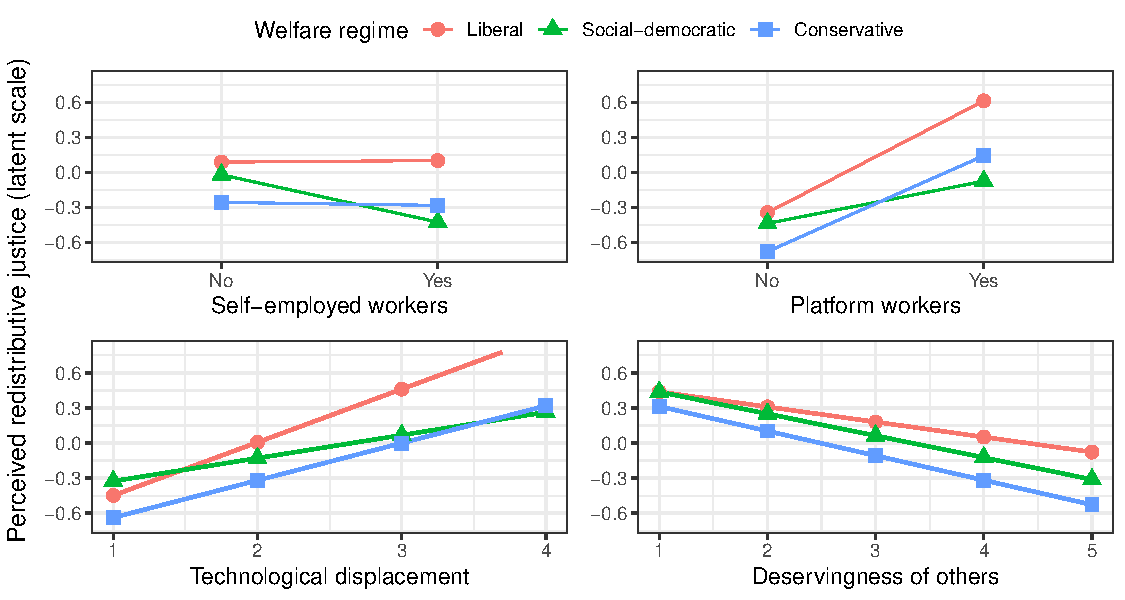
\includegraphics[width=0.85\linewidth,height=\textheight,keepaspectratio]{paper-anonymized_files/figure-pdf/fig-interact-1.pdf}

}

\subcaption{\label{fig-interact}Source: own elaboration with data from
the OECD, Risks That Matter survey 2024.}

}

\end{figure}%

\section{Discussion}\label{discussion}

This article asked whether perceived redistributive justice between
citizens and the state is anchored in labour-market position and in how
workers anticipate technological change, and whether welfare
institutions condition that relationship. The results give qualified
support to the reciprocity framework that motivated the analysis, and
their main interest lies where they depart from the
risk-and-redistribution tradition from which the hypotheses were drawn.
Concern about losing one's job or income and the perception that others
receive undeserved benefits both depress perceived justice (H2, H5),
while perceiving technology as enabling raises it (H4), the largest
effect among the technological perceptions. Two expectations failed.
Non-standard employment was not associated with lower perceived justice,
and platform workers in fact reported higher levels (H1); perceived
displacement risk, expected to erode justice, was positively associated
with it (H3). At the country level, perceived justice proved higher in
richer countries, and the moderation analyses pointed to an
institutional patterning that the regime main effects only partly
capture.

The confirmed hypotheses fit the moral-economy reading on which the
study rests. Workers worried about losing their job or income over the
coming year or two judge the exchange as less just (H2), and those who
see others drawing unearned benefits extend that judgement to their own
relationship with the system (H5), in line with the view that lateral
deservingness assessments and self-referential justice belong to a
single moral economy of welfare (\citeproc{ref-mau_moral_2014}{Mau,
2014}; \citeproc{ref-vanoorschot_making_2006}{Van Oorschot, 2006}). That
the enabling dimension of technology carries the largest effect (H4) is
a reminder that workers do not approach technology only defensively. Its
optimistic pole has received far less attention than its threatening
counterpart, and it matters for welfare attitudes
(\citeproc{ref-autor_why_2015}{Autor, 2015};
\citeproc{ref-brougham_smart_2018}{Brougham and Haar, 2018}).

Self-employment was unrelated to perceived redistributive justice
throughout. This is unsurprising for a category that ranges from
established professionals to precarious own-account workers, whose
contrasting ties to the protection system plausibly offset one another.
The reversal for platform work is harder to set aside, since in the
fully adjusted model platform workers show roughly twice the odds of
reporting higher perceived justice (OR ≈ 2.2). Part of the answer is
compositional. Self-reported platform work in OECD samples is
heterogeneous and captures supplementary and intermittent earners
alongside the platform-dependent (\citeproc{ref-schor_gig_2020}{Schor,
2020}; \citeproc{ref-vallas_what_2020}{Vallas and Schor, 2020}), and the
negative self-employed × platform interaction places the effect among
workers most likely to combine platform earnings with other employment.
The other part is substantive. Perceived redistributive justice is a
judgement of proportionality. Workers loosely attached to the
contributory system contribute little and expect little, so a thin
return can read as proportionate, while formal employees with visible
contributions and clear entitlements may feel short-changed by the same
comparison (\citeproc{ref-schwander_who_2013}{Schwander and Häusermann,
2013}).

The positive association between perceived displacement risk and
perceived redistributive justice (H3) is the departure with the most
theoretical weight. Conceptually, the dependent variable evaluates the
justice of one's own exchange. It does not measure a demand for
redistribution. The literature behind H3 shows that perceived risk
raises the demand for protection
(\citeproc{ref-busemeyer_social_2022}{Busemeyer and Sahm, 2022};
\citeproc{ref-iversen_asset_2001}{Iversen and Soskice, 2001};
\citeproc{ref-thewissen_automation_2019}{Thewissen and Rueda, 2019}),
yet wanting more redistribution and judging the present exchange as just
are analytically distinct, and they need not move together. A worker may
want the state to do more in the face of automation while still
considering that, given what they pay, they receive a just share. The
reversal therefore partly reflects the measurement of a different
attitudinal object, and it reinforces the distinction between
preferences and perceptions on which the article insists
(\citeproc{ref-roosma_just_2016}{Roosma et al., 2016}). Composition also
plays a role. The diffusion of generative artificial intelligence has
extended perceived exposure to formal, higher-skill and digitally
engaged workers (\citeproc{ref-gallego_automation_2022}{Gallego and
Kurer, 2022}), who are precisely the workers with the most continuous
link to the contributory system, so perceived risk now travels together
with relative inclusion. The design of the sample reinforces this
reading. Because the survey only administers these batteries to people
in work, respondents who report high displacement risk are by
construction those still employed despite the exposure they perceive,
while workers already displaced have left the sample. What the
coefficient captures is the judgement of exposed insiders, and exposed
insiders have reasons of their own to view their exchange with the state
favourably.

The moderation patterns are consistent with this reading, though they
should be read with the caution that 27 countries impose on cross-level
estimates. If the positive coefficient reflected institutional
reassurance, it should be largest where protection is most encompassing.
The estimated slope is instead steepest in liberal regimes and flatter
in social-democratic and conservative ones (H8). The time horizon of the
items points the same way. The displacement battery is prospective and
abstract, asking about a five-year horizon, while the job-insecurity
item that behaves as predicted (H2) concerns concrete income loss over
the next year or two. Tangible short-term insecurity erodes perceived
justice. Distant technological prognosis does not, and it may instead
index a reflective engagement with the future of work that comes bundled
with other favourable dispositions
(\citeproc{ref-dekker_fear_2017}{Dekker et al., 2017};
\citeproc{ref-kurer_declining_2020}{Kurer, 2020}). A measurement caveat
remains. Displacement and benefit are positively correlated with each
other (r = 0.48) and with the outcome, and although the factor analysis
separates them, the shared sign suggests a common component of
engagement with the technological frame that future instrumentation
should separate from valence.

The comparative results reshape the regime argument. The strongest
country-level patterning is economic. Perceived redistributive justice
is higher in richer countries, GDP per capita absorbs a substantial
share of the between-country variance, and inequality, unemployment and
social expenditure show no association
(\citeproc{ref-blekesaune_public_2003}{Blekesaune, 2003}). Net of this
composition, regime type orders perceived justice only partially (H6).
The conservative contrast is negative and significant relative to
liberal regimes, while the social-democratic one is indistinguishable, a
pattern at odds with the classic regime hypothesis and consistent with
the heterogeneity already visible in Figure~\ref{fig-cleveland}. All the
regime interactions carry a negative sign, though they only partly match
the expected contrast between universalist and residual regimes. The
positive association of platform work is steepest under liberal
arrangements and flattest under social-democratic ones; the
self-employment effect, predicted to be strongest in residual regimes,
emerges only under social-democratic arrangements (H7); the displacement
effect is dampened in both non-liberal regimes (H8); and the
deservingness gradient is steepest in conservative regimes and
indistinguishable between liberal and social-democratic ones (H9). For
platform work and the technological perceptions, the observed pattern
fits the idea that universalist institutions loosen the connection
between perceived justice and individual labour-market exposure, while
residual, market-tied arrangements keep the two bound together
(\citeproc{ref-larsen_institutional_2008}{Larsen, 2008};
\citeproc{ref-rothstein_just_1998}{Rothstein, 1998}). The
self-employment exception fits the same reciprocity logic once
institutional distance is understood in relative terms. Where dependent
employment is most generously covered, own-account workers stand
furthest from the prevailing standard of protection, and their exchange
with the state reads as comparatively less just
(\citeproc{ref-schwander_who_2013}{Schwander and Häusermann, 2013}). On
this account, regimes matter for how strongly individual circumstances
translate into judgements of justice, while their imprint on the average
level of those judgements is weaker. That structuring role is especially
salient in highly commodified contexts such as the Chilean one
(\citeproc{ref-emmenegger_age_2012}{Emmenegger et al., 2012};
\citeproc{ref-perez-ahumada_conditioning_2026}{Pérez-Ahumada et al.,
2026}).

\section{Conclusion}\label{conclusion}

Drawing on the 2024 wave of the OECD Risks That Matter survey across 27
countries, this article has shown that the perceived redistributive
justice of the fiscal exchange with the welfare state is anchored in the
experience of work, though not in the way the risk-and-redistribution
tradition would predict. Concrete employment insecurity and the
perception that others receive undeserved benefits erode perceived
justice, and perceiving technology as enabling strengthens it.
Non-standard employment, however, does not depress justice, since
platform workers report higher levels, and perceived displacement risk
is positively associated with it. At the country level, perceived
justice is higher in richer countries and, net of that economic
composition, lower in conservative regimes than in liberal ones. The
moderation patterns suggest that universalist welfare institutions
loosen the link between perceived justice and both platform work and
technological perception, while residual arrangements keep it tight;
self-employment, in turn, becomes consequential under universalist
arrangements.

Two implications follow for the comparative study of welfare attitudes.
The first is that perceptions and preferences need to be kept
analytically apart. The same exposure that raises the demand for
redistribution may leave the evaluation of one's own exchange unchanged,
or may even improve it, so findings established for one attitudinal
object cannot be transposed to the other
(\citeproc{ref-roosma_just_2016}{Roosma et al., 2016}). The second
concerns the comparative purchase of welfare-regime theory on these
attitudes. Differences of level between regimes are largely absorbed by
countries' economic composition; what regimes appear to shape is how
strongly individual circumstances translate into judgements of justice.
Reading the regime effect as a matter of structuring, and treating that
reading as a hypothesis for further testing, offers a plausible account
of why the legitimacy of the welfare state fragments along the contours
of the labour market in some institutional settings and holds together
in others.

The findings also bear on the European policy agenda on access to social
protection
(\citeproc{ref-counciloftheeuropeanunion_council_2019}{Council of the
European Union, 2019};
\citeproc{ref-europeanparliamentandcounciloftheeuropeanunion_directive_2024}{European
Parliament and Council of the European Union, 2024}). That platform
workers judge their exchange with the state as comparatively just should
not be read as the absence of a problem. On the proportionality reading
advanced here, it reflects how little they currently contribute to and
expect from the contributory system. Extending coverage, which is the
aim of the Council Recommendation and, for platform work, of the recent
directive, will draw these workers into a fuller exchange in which more
is contributed and more is owed. The legitimacy returns of that
extension will depend on whether the ensuing entitlements are
proportionate to the new contributions and easy for workers to see. The
self-employment finding adds a caution for the most encompassing
systems, since formal inclusion that leaves own-account workers at a
visible distance from the employee standard may end up depressing their
sense of a just exchange.

These conclusions are bounded by the design, and the most consequential
boundary comes from the survey itself. Because the batteries on
employment type and technological perception are only administered to
those in work, the analysis is conditional on employment. It cannot
speak to how the unemployed or the inactive judge their exchange with
the welfare state, although these are the groups for whom that exchange
is most immediately at stake, and it observes technological risk only
among those still employed, the relative survivors of the displacement
it asks about. The data are also cross-sectional, so the analysis
identifies associations only, and reverse causation remains plausible;
those who already regard their exchange as just may simply evaluate
technological change more benignly. The principal independent variables
rest on single items or short scales, and the platform and
self-employment categories are internally heterogeneous, grouping
distinct relationships with the protection system under a common label
(\citeproc{ref-vallas_what_2020}{Vallas and Schor, 2020});
self-identified platform work in online surveys is, in addition, likely
to over-capture marginal and occasional activity
(\citeproc{ref-schor_gig_2020}{Schor, 2020}). The positive correlations
among the technological-perception items signal that the battery does
not fully separate the valence of a perception from engagement with
technological change as a frame. The item on replacement by artificial
intelligence illustrates the point from another angle, since it forms a
perceptual dimension of its own and shows no association with perceived
justice when modelled separately, which suggests an object of perception
that current instruments do not yet capture well. At the macro level, 27
countries afford limited power for cross-level estimation, so the
moderation results are best read as descriptive patterns, and the small
number of cases places a heavy burden on the regime classification,
whose treatment of the post-socialist, southern European and
non-European cases, while defensible, remains open to debate
(\citeproc{ref-aidukaite_welfare_2011}{Aidukaite, 2011};
\citeproc{ref-ferrera_southern_1996}{Ferrera, 1996};
\citeproc{ref-franzoni_welfare_2008}{Martínez Franzoni, 2008}).

Several extensions follow from these limits. Panel data would establish
the temporal ordering of technological perception and perceived
redistributive justice and allow reverse causation to be assessed
directly. Instrumentation that separates concrete from prospective
technological risk, and the valence of a perception from the salience of
technological change, would clarify the mechanisms behind the
displacement result, and qualitative work on how platform and
own-account workers construct the reference points against which they
judge their exchange would do the same for the platform result.
Comparative leverage would improve by complementing categorical regimes
with policy-specific continuous indicators, such as decommodification
and active labour-market and social-investment provision, beyond the
aggregate social expenditure controlled for here. Such indicators would
also permit a more direct test of whether policy feedback underlies the
institutional patterning observed (\citeproc{ref-fan_how_2024}{Fan et
al., 2024}; \citeproc{ref-gallego_automation_2022}{Gallego and Kurer,
2022}). Attention to within-regime heterogeneity, particularly in the
commodified welfare states of Latin America, would test how far the
structuring argument travels beyond the European core
(\citeproc{ref-perez-ahumada_conditioning_2026}{Pérez-Ahumada et al.,
2026}).

In the digital transition, the legitimacy of the welfare state will
partly turn on whether institutions can keep perceived redistributive
justice from fragmenting along individual labour-market lines. The
evidence assembled here is observational, but it points to universalist
designs as better equipped for that task. As digitalisation continues to
remake the standard employment relationship around which social
protection was built
(\citeproc{ref-howcroft_digitalisation_2025}{Howcroft et al., 2025}),
the distribution of perceived justice across the workforce deserves a
place next to the volume of redistribution citizens demand as a question
for the comparative study of welfare legitimacy.

\section{References}\label{references}

\protect\phantomsection\label{refs}
\begin{CSLReferences}{1}{1}
\bibitem[\citeproctext]{ref-aidukaite_welfare_2011}
Aidukaite J (2011)
\href{https://doi.org/10.1016/j.postcomstud.2011.07.005}{Welfare reforms
and socio-economic trends in the 10 new {EU} member states of {Central}
and {Eastern Europe}}. \emph{Communist and Post-Communist Studies}
44(3): 211--219.

\bibitem[\citeproctext]{ref-anderson_workers_2007}
Anderson CJ and Pontusson J (2007)
\href{https://doi.org/10.1111/j.1475-6765.2007.00692.x}{Workers, worries
and welfare states: {Social} protection and job insecurity in 15 {OECD}
countries}. \emph{European Journal of Political Research} 46(2):
211--235.

\bibitem[\citeproctext]{ref-arntz_risk_2016}
Arntz M, Gregory T and Zierahn U (2016)
\emph{\href{https://doi.org/10.1787/5jlz9h56dvq7-en}{The {Risk} of
{Automation} for {Jobs} in {OECD Countries}: {A Comparative Analysis}}}.
{OECD Social}, {Employment} and {Migration Working Papers} 189, \{\{OECD
Social\}\}, \{\{Employment\}\} and \{\{Migration Working Papers\}\},
May.

\bibitem[\citeproctext]{ref-arts_three_2002}
Arts W and Gelissen J (2002)
\href{https://doi.org/10.1177/0952872002012002114}{Three worlds of
welfare capitalism or more? {A} state-of-the-art report}. \emph{Journal
of European Social Policy} 12(2): 137--158.

\bibitem[\citeproctext]{ref-autor_why_2015}
Autor DH (2015) \href{https://doi.org/10.1257/jep.29.3.3}{Why {Are There
Still So Many Jobs}? {The History} and {Future} of {Workplace
Automation}}. \emph{Journal of Economic Perspectives} 29(3): 3--30.

\bibitem[\citeproctext]{ref-bambra_sifting_2007}
Bambra C (2007)
\href{https://doi.org/10.1111/j.1467-9515.2007.00536.x}{{`{Sifting} the
{Wheat} from the {Chaff}'}: {A Two}-dimensional {Discriminant Analysis}
of {Welfare State Regime Theory}}. \emph{Social Policy \&
Administration} 41(1): 1--28.

\bibitem[\citeproctext]{ref-behrendt_social_2019}
Behrendt C, Nguyen QA and Rani U (2019)
\href{https://doi.org/10.1111/issr.12212}{Social protection systems and
the future of work: {Ensuring} social security for digital platform
workers}. \emph{International Social Security Review} 72(3): 17--41.

\bibitem[\citeproctext]{ref-blekesaune_public_2003}
Blekesaune M (2003) \href{https://doi.org/10.1093/esr/19.5.415}{Public
{Attitudes} toward {Welfare State Policies}: {A Comparative Analysis} of
24 {Nations}}. \emph{European Sociological Review} 19(5): 415--427.

\bibitem[\citeproctext]{ref-brougham_smart_2018}
Brougham D and Haar J (2018)
\href{https://doi.org/10.1017/jmo.2016.55}{Smart {Technology},
{Artificial Intelligence}, {Robotics}, and {Algorithms} ({STARA}):
{Employees}' perceptions of our future workplace}. \emph{Journal of
Management \& Organization} 24(2): 239--257.

\bibitem[\citeproctext]{ref-busemeyer_social_2022}
Busemeyer MR and Sahm AHJ (2022)
\href{https://doi.org/10.1017/S0047279421000519}{Social {Investment},
{Redistribution} or {Basic Income}? {Exploring} the {Association Between
Automation Risk} and {Welfare State Attitudes} in {Europe}}.
\emph{Journal of Social Policy} 51(4): 751--770.

\bibitem[\citeproctext]{ref-bustelo_automation_2020}
Bustelo M, Egaña Del Sol P, Ripani L, et al. (2020)
\emph{\href{https://doi.org/10.18235/0002566}{Automation in {Latin
America}: {Are Women} at {Higher Risk} of {Losing Their Jobs}?}} August.
Inter-American Development Bank.

\bibitem[\citeproctext]{ref-castillo_perception_2022}
Castillo J-C, García-Castro J-D and Venegas M (2022)
\href{https://doi.org/10.1080/02134748.2021.2009275}{Perception of
economic inequality: Concepts, associated factors and prospects of a
burgeoning research agenda ({Percepción} de desigualdad económica:
Conceptos, factores asociados y proyecciones de una agenda creciente de
investigación)}. \emph{International Journal of Social Psychology:
Revista de Psicología Social} 37(1): 180--207.

\bibitem[\citeproctext]{ref-castillo_perceptions_2025}
Castillo JC, Laffert A, Carrasco K, et al. (2025)
\href{https://doi.org/10.3389/fsoc.2025.1634219}{Perceptions of
inequality and meritocracy: Their interplay in shaping preferences for
market justice in {Chile} (2016--2023)}. \emph{Frontiers in Sociology}
10: 1634219.

\bibitem[\citeproctext]{ref-cavaille_fair_2025}
Cavaillé C (2025)
\emph{\href{https://doi.org/10.1017/9781009366038}{Fair {Enough}?:
{Support} for {Redistribution} in the {Age} of {Inequality}}}. 1st edn
Cambridge University Press.

\bibitem[\citeproctext]{ref-haubo_cumulative_2018}
Christensen RHB (2018) Cumulative link models for ordinal regression
with the {R} package ordinal. In: 2018.

\bibitem[\citeproctext]{ref-chung_institutions_2011}
Chung H and Van Oorschot W (2011)
\href{https://doi.org/10.1177/0958928711412224}{Institutions versus
market forces: {Explaining} the employment insecurity of {European}
individuals during (the beginning of) the financial crisis}.
\emph{Journal of European Social Policy} 21(4): 287--301.

\bibitem[\citeproctext]{ref-counciloftheeuropeanunion_council_2019}
Council of the European Union (2019) Council {Recommendation} of 8
{November} 2019 on access to social protection for workers and the
self-employed (2019/{C} 387/01). Official Journal of the European Union,
C 387, 15 November 2019, pp. 1--8.

\bibitem[\citeproctext]{ref-cusack_risks_2006}
Cusack T, Iversen T and Rehm P (2006)
\href{https://doi.org/10.1093/oxrep/grj022}{Risks at {Work}: {The
Demand} and {Supply Sides} of {Government Redistribution}}. \emph{Oxford
Review of Economic Policy} 22(3): 365--389.

\bibitem[\citeproctext]{ref-dewitte_job_2005}
De Witte H (2005) \href{https://doi.org/10.4102/sajip.v31i4.200}{Job
insecurity: {Review} of the international literature on definitions,
prevalence, antecedents and consequences}. \emph{SA Journal of
Industrial Psychology} 31(4).

\bibitem[\citeproctext]{ref-dekker_fear_2017}
Dekker F, Salomons A and Waal JVD (2017)
\href{https://doi.org/10.1093/ser/mwx005}{Fear of robots at work: The
role of economic self-interest}. \emph{Socio-Economic Review} 15(3):
539--562.

\bibitem[\citeproctext]{ref-emmenegger_age_2012}
Emmenegger P, Häusermann S, Palier B, et al. (2012)
\emph{\href{https://doi.org/10.5167/UZH-65793}{The Age of Dualization :
The Changing Face of Inequality in Deindustrializing Societies}} (eds P
Emmenegger, S Häusermann, B Palier, et al.). Oxford University Press.

\bibitem[\citeproctext]{ref-esping-andersen_three_1993}
Esping-Andersen G (1990) \emph{The Three Worlds of Welfare Capitalism}.
Cambridge: Polity press.

\bibitem[\citeproctext]{ref-europeanparliamentandcounciloftheeuropeanunion_directive_2024}
European Parliament and Council of the European Union (2024) Directive
({EU}) 2024/2831 of the {European Parliament} and of the {Council} of 23
{October} 2024 on improving working conditions in platform work ({Text}
with {EEA} relevance). Official Journal of the European Union, L series,
11 November 2024.

\bibitem[\citeproctext]{ref-fan_how_2024}
Fan Z, Ning J and He AJ (2024)
\href{https://doi.org/10.1017/S1474746422000513}{How {Does Automation
Risk Shape Social Policy Preference}? {Employment Insecurity} and
{Policy Feedback Effect} in {China}}. \emph{Social Policy and Society}
23(3): 750--768.

\bibitem[\citeproctext]{ref-Fenger2006WelfareRI}
Fenger HJM (2006) Welfare regimes in central and eastern europe:
{Incorporating} post-communist countries in a welfare regime typology.
In: 2006.

\bibitem[\citeproctext]{ref-ferrera_southern_1996}
Ferrera M (1996) \href{https://doi.org/10.1177/095892879600600102}{The
'{Southern Model}' of {Welfare} in {Social Europe}}. \emph{Journal of
European Social Policy} 6(1): 17--37.

\bibitem[\citeproctext]{ref-finseraas_income_2009}
Finseraas H (2009)
\href{https://doi.org/10.1111/j.1467-9477.2008.00211.x}{Income
{Inequality} and {Demand} for {Redistribution}: {A Multilevel Analysis}
of {European Public Opinion}}. \emph{Scandinavian Political Studies}
32(1): 94--119.

\bibitem[\citeproctext]{ref-frey_future_2017}
Frey CB and Osborne MA (2017)
\href{https://doi.org/10.1016/j.techfore.2016.08.019}{The future of
employment: {How} susceptible are jobs to computerisation?}
\emph{Technological Forecasting and Social Change} 114: 254--280.

\bibitem[\citeproctext]{ref-gallego_automation_2022}
Gallego A and Kurer T (2022)
\href{https://doi.org/10.1146/annurev-polisci-051120-104535}{Automation,
{Digitalization}, and {Artificial Intelligence} in the {Workplace}:
{Implications} for {Political Behavior}}. \emph{Annual Review of
Political Science} 25(1): 463--484.

\bibitem[\citeproctext]{ref-gallie_economic_2013}
Gallie D (ed.) (2013)
\emph{\href{https://doi.org/10.1093/acprof:oso/9780199664719.001.0001}{Economic
{Crisis}, {Quality} of {Work}, and {Social Integration}: {The European
Experience}}}. Oxford University Press.

\bibitem[\citeproctext]{ref-garcia-castro_perceiving_2020}
García-Castro JD, Rodríguez-Bailón R and Willis GB (2020)
\href{https://doi.org/10.1016/j.jesp.2020.104019}{Perceiving economic
inequality in everyday life decreases tolerance to inequality}.
\emph{Journal of Experimental Social Psychology} 90: 104019.

\bibitem[\citeproctext]{ref-garcia-sanchez_attitudes_2020}
García-Sánchez E, Osborne D, Willis GB, et al. (2020)
\href{https://doi.org/10.1111/bjso.12326}{Attitudes towards
redistribution and the interplay between perceptions and beliefs about
inequality}. \emph{British Journal of Social Psychology} 59(1):
111--136.

\bibitem[\citeproctext]{ref-gimpelson_misperceiving_2018}
Gimpelson V and Treisman D (2018)
\href{https://doi.org/10.1111/ecpo.12103}{Misperceiving inequality}.
\emph{Economics \& Politics} 30(1): 27--54.

\bibitem[\citeproctext]{ref-gutierrezcrocco_effects_2022}
Gutiérrez Crocco F and Atzeni M (2022)
\href{https://doi.org/10.1111/ilr.12376}{The effects of the pandemic on
gig economy couriers in {Argentina} and {Chile}: {Precarity},
algorithmic control and mobilization}. \emph{International Labour
Review} 161(3): 441--461.

\bibitem[\citeproctext]{ref-howcroft_digitalisation_2025}
Howcroft D, Banister E, Jarvis-King L, et al. (2025)
\href{https://doi.org/10.1177/09500170241301015}{Digitalisation and the
{Remaking} of the {Ideal Worker}}. \emph{Work, Employment and Society}
39(3): 703--726.

\bibitem[\citeproctext]{ref-hox_multilevel_2017}
Hox JJ, Moerbeek M and Van De Schoot R (2017)
\emph{\href{https://doi.org/10.4324/9781315650982}{Multilevel
{Analysis}: {Techniques} and {Applications}}}. 3rd edn Third edition.
\textbar{} New York, NY : Routledge, 2017. \textbar: Routledge.

\bibitem[\citeproctext]{ref-im_losers_2019}
Im ZJ, Mayer N, Palier B, et al. (2019)
\href{https://doi.org/10.1177/2053168018822395}{The {`losers of
automation'}: {A} reservoir of votes for the radical right?}
\emph{Research \& Politics} 6(1): 2053168018822395.

\bibitem[\citeproctext]{ref-iversen_asset_2001}
Iversen T and Soskice D (2001)
\href{https://doi.org/10.1017/S0003055400400079}{An {Asset Theory} of
{Social Policy Preferences}}. \emph{American Political Science Review}
95(4): 875--893.

\bibitem[\citeproctext]{ref-jaeger_welfare_2006}
Jæger MM (2006) \href{https://doi.org/10.1093/esr/jci049}{Welfare
{Regimes} and {Attitudes Towards Redistribution}: {The Regime Hypothesis
Revisited}}. \emph{European Sociological Review} 22(2): 157--170.

\bibitem[\citeproctext]{ref-kalleberg_good_2011}
Kalleberg A (2011) \emph{Good Jobs, Bad Jobs: {The} Rise of Polarized
and Precarious Employment Systems in the {United States}, 1970s-2000s}.

\bibitem[\citeproctext]{ref-kenworthy_inequality_2007}
Kenworthy L and McCall L (2007)
\href{https://doi.org/10.1093/ser/mwm006}{Inequality, public opinion and
redistribution}. \emph{Socio-Economic Review} 6(1): 35--68.

\bibitem[\citeproctext]{ref-korpi_paradox_1998}
Korpi W and Palme J (1998) \href{https://doi.org/10.2307/2657333}{The
{Paradox} of {Redistribution} and {Strategies} of {Equality}: {Welfare
State Institutions}, {Inequality}, and {Poverty} in the {Western
Countries}}. \emph{American Sociological Review} 63(5): 661.

\bibitem[\citeproctext]{ref-kurer_declining_2020}
Kurer T (2020) \href{https://doi.org/10.1177/0010414020912283}{The
{Declining Middle}: {Occupational Change}, {Social Status}, and the
{Populist Right}}. \emph{Comparative Political Studies} 53(10-11):
1798--1835.

\bibitem[\citeproctext]{ref-laenen_welfare_2020}
Laenen T (2020) \emph{Welfare Deservingness and Welfare Policy: Popular
Deservingness Opinions and Their Interaction with Welfare State
Policies}. Cheltenham, UK Northampton, MA, USA: Edward Elgar Publishing.

\bibitem[\citeproctext]{ref-larsen_institutional_2008}
Larsen CA (2008) \href{https://doi.org/10.1177/0010414006295234}{The
{Institutional Logic} of {Welfare Attitudes}: {How Welfare Regimes
Influence Public Support}}. \emph{Comparative Political Studies} 41(2):
145--168.

\bibitem[\citeproctext]{ref-lenth_emmeans_2017}
Lenth RV and Piaskowski J (2017)
\href{https://doi.org/10.32614/CRAN.package.emmeans}{Emmeans: {Estimated
Marginal Means}, aka {Least-Squares Means}}. Comprehensive R Archive
Network.

\bibitem[\citeproctext]{ref-lindh_class_2020}
Lindh A and McCall L (2020)
\href{https://doi.org/10.1146/annurev-soc-121919-054609}{Class
{Position} and {Political Opinion} in {Rich Democracies}}. \emph{Annual
Review of Sociology} 46(1): 419--441.

\bibitem[\citeproctext]{ref-franzoni_welfare_2008}
Martínez Franzoni J (2008)
\href{https://doi.org/10.1111/j.1548-2456.2008.00013.x}{Welfare
{Regimes} in {Latin America}: {Capturing Constellations} of {Markets},
{Families}, and {Policies}}. \emph{Latin American Politics and Society}
50(02): 67--100.

\bibitem[\citeproctext]{ref-marx_effect_2014}
Marx P (2014) \href{https://doi.org/10.1177/0958928714538217}{The effect
of job insecurity and employability on preferences for redistribution in
{Western Europe}}. \emph{Journal of European Social Policy} 24(4):
351--366.

\bibitem[\citeproctext]{ref-mau_moral_2014}
Mau S (2014) \emph{The Moral Economy of Welfare States: {Britain} and
{Germany} Compared}. First issued in paperback. Routledge/{EUI} studies
in the political economy of welfare 5. London New York NY: Routledge \&
Francis Group.

\bibitem[\citeproctext]{ref-mccall_undeserving_2013}
McCall L (2013)
\emph{\href{https://doi.org/10.1017/CBO9781139225687}{The {Undeserving
Rich}: {American Beliefs} about {Inequality}, {Opportunity}, and
{Redistribution}}}. 1st edn Cambridge University Press.

\bibitem[\citeproctext]{ref-mijs_paradox_2021}
Mijs JJB (2021) \href{https://doi.org/10.1093/ser/mwy051}{The paradox of
inequality: Income inequality and belief in meritocracy go hand in
hand}. \emph{Socio-Economic Review} 19(1): 7--35.

\bibitem[\citeproctext]{ref-oecd_risks_2024}
OECD (2024) Risks that {Matter Survey}: 2024 {Public Use Microdata
File}. {Available} via {http://oe.cd/rtm}.

\bibitem[\citeproctext]{ref-osberg_fair_2006}
Osberg L and Smeeding T (2006)
\href{https://doi.org/10.1177/000312240607100305}{{`{Fair}'}
{Inequality}? {Attitudes} toward {Pay Differentials}: {The United
States} in {Comparative Perspective}}. \emph{American Sociological
Review} 71(3): 450--473.

\bibitem[\citeproctext]{ref-perez_building_2023}
Pérez-Ahumada P (2023) \emph{Building Power to Shape Labor Policy:
Unions, Employer Associations, and Reform in Neoliberal {Chile}}. Pitt
{Latin American} series. Pittsburgh (Pa.): University of Pittsburgh
Press.

\bibitem[\citeproctext]{ref-perez-ahumada_conditioning_2026}
Pérez-Ahumada P, Olivares-Collío D and Carrasco K (2026)
\href{https://doi.org/10.1177/08969205261417585}{The conditioning power
of class: {Collective} action and attitudes toward inequality in
neoliberal {Chile} (2016--2023)}. \emph{Critical Sociology}:
08969205261417585.

\bibitem[\citeproctext]{ref-petersen_social_2012}
Petersen MB (2012)
\href{https://doi.org/10.1111/j.1540-5907.2011.00545.x}{Social {Welfare}
as {Small}-{Scale Help}: {Evolutionary Psychology} and the
{Deservingness Heuristic}}. \emph{American Journal of Political Science}
56(1): 1--16.

\bibitem[\citeproctext]{ref-reeskens_equity_2013}
Reeskens T and Van Oorschot W (2013)
\href{https://doi.org/10.1080/13501763.2012.752064}{Equity, equality, or
need? {A} study of popular preferences for welfare redistribution
principles across 24 {European} countries}. \emph{Journal of European
Public Policy} 20(8): 1174--1195.

\bibitem[\citeproctext]{ref-rehm_risks_2009}
Rehm P (2009) \href{https://doi.org/10.1177/0010414008330595}{Risks and
{Redistribution}: {An Individual-Level Analysis}}. \emph{Comparative
Political Studies} 42(7): 855--881.

\bibitem[\citeproctext]{ref-roosma_just_2016}
Roosma F, Van Oorschot W and Gelissen J (2016)
\href{https://doi.org/10.1093/ijpor/edv020}{A {Just Distribution} of
{Burdens}? {Attitudes Toward} the {Social Distribution} of {Taxes} in 26
{Welfare States}}. \emph{International Journal of Public Opinion
Research} 28(3): 376--400.

\bibitem[\citeproctext]{ref-rothstein_just_1998}
Rothstein B (1998)
\emph{\href{https://doi.org/10.1017/CBO9780511598449}{Just {Institutions
Matter}: {The Moral} and {Political Logic} of the {Universal Welfare
State}}}. 1st edn Cambridge University Press.

\bibitem[\citeproctext]{ref-rueda_social_2007}
Rueda D (2007)
\emph{\href{https://doi.org/10.1093/acprof:oso/9780199216352.001.0001}{Social
{Democracy Inside Out}: {Partisanship} and {Labor Market Policy} in
{Advanced Industrialized Democracies}}}. 1st edn Oxford University
PressOxford.

\bibitem[\citeproctext]{ref-schmidt-catran_economic_2016}
Schmidt-Catran AW (2016)
\href{https://doi.org/10.1093/ser/mwu030}{Economic inequality and public
demand for redistribution: Combining cross-sectional and longitudinal
evidence}. \emph{Socio-Economic Review} 14(1): 119--140.

\bibitem[\citeproctext]{ref-schor_gig_2020}
Schor JB (2020) \emph{After the Gig: How the Sharing Economy Got
Hijacked and How to Win It Back}. Oakland, California: University of
California Press.

\bibitem[\citeproctext]{ref-schwander_who_2013}
Schwander H and Häusermann S (2013)
\href{https://doi.org/10.1177/0958928713480064}{Who is in and who is
out? {A} risk-based conceptualization of insiders and outsiders}.
\emph{Journal of European Social Policy} 23(3): 248--269.

\bibitem[\citeproctext]{ref-snijders_multilevel_2012}
Snijders TAB and Bosker RJ (2012) \emph{Multilevel Analysis: An
Introduction to Basic and Advanced Multilevel Modeling}. 2nd ed. Los
Angeles: Sage.

\bibitem[\citeproctext]{ref-standing_precariat_2014}
Standing G (2014) \emph{The Precariat: The New Dangerous Class}. London,
UK ; New York, NY: Bloomsbury.

\bibitem[\citeproctext]{ref-svallfors_worlds_1997}
Svallfors S (1997)
\href{https://doi.org/10.1093/oxfordjournals.esr.a018219}{Worlds of
{Welfare} and {Attitudes} to {Redistribution}: {A Comparison} of {Eight
Western Nations}}. \emph{European Sociological Review} 13(3): 283--304.

\bibitem[\citeproctext]{ref-svallfors_government_2013}
Svallfors S (2013)
\href{https://doi.org/10.1017/S175577391200015X}{Government quality,
egalitarianism, and attitudes to taxes and social spending: A {European}
comparison}. \emph{European Political Science Review} 5(3): 363--380.

\bibitem[\citeproctext]{ref-sverke_no_2002}
Sverke M, Hellgren J and Näswall K (2002)
\href{https://doi.org/10.1037/1076-8998.7.3.242}{No security: {A}
meta-analysis and review of job insecurity and its consequences.}
\emph{Journal of Occupational Health Psychology} 7(3): 242--264.

\bibitem[\citeproctext]{ref-thewissen_automation_2019}
Thewissen S and Rueda D (2019)
\href{https://doi.org/10.1177/0010414017740600}{Automation and the
{Welfare State}: {Technological Change} as a {Determinant} of
{Redistribution Preferences}}. \emph{Comparative Political Studies}
52(2): 171--208.

\bibitem[\citeproctext]{ref-thomas_survey_2025}
Thomas J, Frey V and Clarke C (2025)
\emph{\href{https://doi.org/10.1787/5eebe551-en}{Survey design and
technical documentation supporting the {OECD Risks} that {Matter
Survey}}}. 324th edn {OECD Social}, {Employment} and {Migration Working
Papers}, \{\{OECD Social\}\}, \{\{Employment\}\} and \{\{Migration
Working Papers\}\}, June.

\bibitem[\citeproctext]{ref-vallas_what_2020}
Vallas S and Schor JB (2020)
\href{https://doi.org/10.1146/annurev-soc-121919-054857}{What {Do
Platforms Do}? {Understanding} the {Gig Economy}}. \emph{Annual Review
of Sociology} 46(1): 273--294.

\bibitem[\citeproctext]{ref-oorschot_who_2000}
Van Oorschot W (2000)
\href{https://doi.org/10.1332/0305573002500811}{Who should get what, and
why? {On} deservingness criteria and the conditionality of solidarity
among the public}. \emph{Policy \& Politics} 28(1): 33--48.

\bibitem[\citeproctext]{ref-vanoorschot_making_2006}
Van Oorschot W (2006)
\href{https://doi.org/10.1177/0958928706059829}{Making the difference in
social {Europe}: Deservingness perceptions among citizens of {European}
welfare states}. \emph{Journal of European Social Policy} 16(1): 23--42.

\bibitem[\citeproctext]{ref-vanoorschot_social_2017}
Van Oorschot W, Roosma F, Meuleman B, et al. (eds) (2017)
\emph{\href{https://doi.org/10.4337/9781785367212}{The {Social
Legitimacy} of {Targeted Welfare}: {Attitudes} to {Welfare
Deservingness}}}. Edward Elgar Publishing.

\bibitem[\citeproctext]{ref-wood_good_2019}
Wood AJ, Graham M, Lehdonvirta V, et al. (2019)
\href{https://doi.org/10.1177/0950017018785616}{Good {Gig}, {Bad Gig}:
{Autonomy} and {Algorithmic Control} in the {Global Gig Economy}}.
\emph{Work, Employment and Society} 33(1): 56--75.

\end{CSLReferences}

\section{Appendix}\label{appendix}



\subsection{Dimensions of Perceived technological
change}\label{dimensions-of-perceived-technological-change}

{

\begin{longtable}[]{@{}
  >{\raggedright\arraybackslash}p{(\linewidth - 6\tabcolsep) * \real{0.2500}}
  >{\raggedright\arraybackslash}p{(\linewidth - 6\tabcolsep) * \real{0.2500}}
  >{\raggedright\arraybackslash}p{(\linewidth - 6\tabcolsep) * \real{0.2500}}
  >{\raggedright\arraybackslash}p{(\linewidth - 6\tabcolsep) * \real{0.2500}}@{}}

\caption{\label{tbl-efa}Exploratory factor analysis of Perceived
technological change items}

\tabularnewline

\toprule\noalign{}
\endhead
\bottomrule\noalign{}
\endlastfoot
~ & Factor 1 & Factor 2 & Factor 3 \\
Replaced by robot & 0.76 & -0.03 & 0.10 \\
Replaced by AI & 0.30 & 0.02 & 0.76 \\
\begin{minipage}[t]{\linewidth}\raggedright
Job replaced by person on\\
internet platform\strut
\end{minipage} & 0.77 & 0.04 & 0.00 \\
Lose job due to skills & 0.78 & -0.01 & -0.04 \\
\begin{minipage}[t]{\linewidth}\raggedright
Tech will improve work-life\\
balance\strut
\end{minipage} & -0.08 & 0.77 & 0.04 \\
Tech will make work safer & 0.18 & 0.61 & -0.04 \\
\begin{minipage}[t]{\linewidth}\raggedright
Tech will make work less\\
boring/stressful/demanding\strut
\end{minipage} & -0.03 & 0.78 & -0.00 \\
Cronbach\textquotesingle s α & 0.83 & 0.78 & \\

\end{longtable}

}

\subsection{Country classification and N
samples}\label{country-classification-and-n-samples}

\global\setlength{\Oldarrayrulewidth}{\arrayrulewidth}

\global\setlength{\Oldtabcolsep}{\tabcolsep}

\setlength{\tabcolsep}{2pt}

\renewcommand*{\arraystretch}{1.5}



\providecommand{\ascline}[3]{\noalign{\global\arrayrulewidth #1}\arrayrulecolor[HTML]{#2}\cline{#3}}

\begin{longtable}[c]{|p{1.50in}|p{1.34in}|p{0.87in}|p{0.87in}}

\caption{\label{tbl-classification}Welfare regime classification and
sample sizes by country}

\tabularnewline

\ascline{1.5pt}{666666}{1-4}

\multicolumn{1}{>{\raggedright}m{\dimexpr 1.5in+0\tabcolsep}}{\textcolor[HTML]{000000}{\fontsize{9}{8}\selectfont{Welfare\ regime}}} & \multicolumn{1}{>{\raggedright}m{\dimexpr 1.34in+0\tabcolsep}}{\textcolor[HTML]{000000}{\fontsize{9}{8}\selectfont{Country}}} & \multicolumn{1}{>{\raggedleft}m{\dimexpr 0.87in+0\tabcolsep}}{\textcolor[HTML]{000000}{\fontsize{9}{8}\selectfont{Original\ N}}} & \multicolumn{1}{>{\raggedleft}m{\dimexpr 0.87in+0\tabcolsep}}{\textcolor[HTML]{000000}{\fontsize{9}{8}\selectfont{Final\ N}}} \\

\ascline{1.5pt}{666666}{1-4}\endfirsthead 

\ascline{1.5pt}{666666}{1-4}

\multicolumn{1}{>{\raggedright}m{\dimexpr 1.5in+0\tabcolsep}}{\textcolor[HTML]{000000}{\fontsize{9}{8}\selectfont{Welfare\ regime}}} & \multicolumn{1}{>{\raggedright}m{\dimexpr 1.34in+0\tabcolsep}}{\textcolor[HTML]{000000}{\fontsize{9}{8}\selectfont{Country}}} & \multicolumn{1}{>{\raggedleft}m{\dimexpr 0.87in+0\tabcolsep}}{\textcolor[HTML]{000000}{\fontsize{9}{8}\selectfont{Original\ N}}} & \multicolumn{1}{>{\raggedleft}m{\dimexpr 0.87in+0\tabcolsep}}{\textcolor[HTML]{000000}{\fontsize{9}{8}\selectfont{Final\ N}}} \\

\ascline{1.5pt}{666666}{1-4}\endhead



\multicolumn{1}{>{\raggedright}p{\dimexpr 1.5in+0\tabcolsep}}{} & \multicolumn{1}{>{\raggedright}m{\dimexpr 1.34in+0\tabcolsep}}{\textcolor[HTML]{000000}{\fontsize{9}{8}\selectfont{Canada}}} & \multicolumn{1}{>{\raggedleft}m{\dimexpr 0.87in+0\tabcolsep}}{\textcolor[HTML]{000000}{\fontsize{9}{8}\selectfont{1,009}}} & \multicolumn{1}{>{\raggedleft}m{\dimexpr 0.87in+0\tabcolsep}}{\textcolor[HTML]{000000}{\fontsize{9}{8}\selectfont{794}}} \\





\multicolumn{1}{>{\raggedright}p{\dimexpr 1.5in+0\tabcolsep}}{} & \multicolumn{1}{>{\raggedright}m{\dimexpr 1.34in+0\tabcolsep}}{\textcolor[HTML]{000000}{\fontsize{9}{8}\selectfont{Chile}}} & \multicolumn{1}{>{\raggedleft}m{\dimexpr 0.87in+0\tabcolsep}}{\textcolor[HTML]{000000}{\fontsize{9}{8}\selectfont{1,002}}} & \multicolumn{1}{>{\raggedleft}m{\dimexpr 0.87in+0\tabcolsep}}{\textcolor[HTML]{000000}{\fontsize{9}{8}\selectfont{657}}} \\





\multicolumn{1}{>{\raggedright}p{\dimexpr 1.5in+0\tabcolsep}}{} & \multicolumn{1}{>{\raggedright}m{\dimexpr 1.34in+0\tabcolsep}}{\textcolor[HTML]{000000}{\fontsize{9}{8}\selectfont{Estonia}}} & \multicolumn{1}{>{\raggedleft}m{\dimexpr 0.87in+0\tabcolsep}}{\textcolor[HTML]{000000}{\fontsize{9}{8}\selectfont{1,001}}} & \multicolumn{1}{>{\raggedleft}m{\dimexpr 0.87in+0\tabcolsep}}{\textcolor[HTML]{000000}{\fontsize{9}{8}\selectfont{761}}} \\





\multicolumn{1}{>{\raggedright}p{\dimexpr 1.5in+0\tabcolsep}}{} & \multicolumn{1}{>{\raggedright}m{\dimexpr 1.34in+0\tabcolsep}}{\textcolor[HTML]{000000}{\fontsize{9}{8}\selectfont{Ireland}}} & \multicolumn{1}{>{\raggedleft}m{\dimexpr 0.87in+0\tabcolsep}}{\textcolor[HTML]{000000}{\fontsize{9}{8}\selectfont{1,004}}} & \multicolumn{1}{>{\raggedleft}m{\dimexpr 0.87in+0\tabcolsep}}{\textcolor[HTML]{000000}{\fontsize{9}{8}\selectfont{812}}} \\





\multicolumn{1}{>{\raggedright}p{\dimexpr 1.5in+0\tabcolsep}}{} & \multicolumn{1}{>{\raggedright}m{\dimexpr 1.34in+0\tabcolsep}}{\textcolor[HTML]{000000}{\fontsize{9}{8}\selectfont{Latvia}}} & \multicolumn{1}{>{\raggedleft}m{\dimexpr 0.87in+0\tabcolsep}}{\textcolor[HTML]{000000}{\fontsize{9}{8}\selectfont{1,010}}} & \multicolumn{1}{>{\raggedleft}m{\dimexpr 0.87in+0\tabcolsep}}{\textcolor[HTML]{000000}{\fontsize{9}{8}\selectfont{695}}} \\





\multicolumn{1}{>{\raggedright}p{\dimexpr 1.5in+0\tabcolsep}}{} & \multicolumn{1}{>{\raggedright}m{\dimexpr 1.34in+0\tabcolsep}}{\textcolor[HTML]{000000}{\fontsize{9}{8}\selectfont{Lithuania}}} & \multicolumn{1}{>{\raggedleft}m{\dimexpr 0.87in+0\tabcolsep}}{\textcolor[HTML]{000000}{\fontsize{9}{8}\selectfont{1,006}}} & \multicolumn{1}{>{\raggedleft}m{\dimexpr 0.87in+0\tabcolsep}}{\textcolor[HTML]{000000}{\fontsize{9}{8}\selectfont{748}}} \\





\multicolumn{1}{>{\raggedright}p{\dimexpr 1.5in+0\tabcolsep}}{} & \multicolumn{1}{>{\raggedright}m{\dimexpr 1.34in+0\tabcolsep}}{\textcolor[HTML]{000000}{\fontsize{9}{8}\selectfont{Mexico}}} & \multicolumn{1}{>{\raggedleft}m{\dimexpr 0.87in+0\tabcolsep}}{\textcolor[HTML]{000000}{\fontsize{9}{8}\selectfont{1,011}}} & \multicolumn{1}{>{\raggedleft}m{\dimexpr 0.87in+0\tabcolsep}}{\textcolor[HTML]{000000}{\fontsize{9}{8}\selectfont{645}}} \\





\multicolumn{1}{>{\raggedright}p{\dimexpr 1.5in+0\tabcolsep}}{} & \multicolumn{1}{>{\raggedright}m{\dimexpr 1.34in+0\tabcolsep}}{\textcolor[HTML]{000000}{\fontsize{9}{8}\selectfont{United\ Kingdom}}} & \multicolumn{1}{>{\raggedleft}m{\dimexpr 0.87in+0\tabcolsep}}{\textcolor[HTML]{000000}{\fontsize{9}{8}\selectfont{1,010}}} & \multicolumn{1}{>{\raggedleft}m{\dimexpr 0.87in+0\tabcolsep}}{\textcolor[HTML]{000000}{\fontsize{9}{8}\selectfont{760}}} \\





\multicolumn{1}{>{\raggedright}p{\dimexpr 1.5in+0\tabcolsep}}{\multirow[t]{-9}{*}{\parbox{1.5in}{\raggedright \textcolor[HTML]{000000}{\fontsize{9}{8}\selectfont{Liberal}}}}} & \multicolumn{1}{>{\raggedright}m{\dimexpr 1.34in+0\tabcolsep}}{\textcolor[HTML]{000000}{\fontsize{9}{8}\selectfont{United\ States}}} & \multicolumn{1}{>{\raggedleft}m{\dimexpr 0.87in+0\tabcolsep}}{\textcolor[HTML]{000000}{\fontsize{9}{8}\selectfont{1,005}}} & \multicolumn{1}{>{\raggedleft}m{\dimexpr 0.87in+0\tabcolsep}}{\textcolor[HTML]{000000}{\fontsize{9}{8}\selectfont{691}}} \\

\ascline{1pt}{666666}{1-4}



\multicolumn{1}{>{\raggedright}p{\dimexpr 1.5in+0\tabcolsep}}{} & \multicolumn{1}{>{\raggedright}m{\dimexpr 1.34in+0\tabcolsep}}{\textcolor[HTML]{000000}{\fontsize{9}{8}\selectfont{Denmark}}} & \multicolumn{1}{>{\raggedleft}m{\dimexpr 0.87in+0\tabcolsep}}{\textcolor[HTML]{000000}{\fontsize{9}{8}\selectfont{1,006}}} & \multicolumn{1}{>{\raggedleft}m{\dimexpr 0.87in+0\tabcolsep}}{\textcolor[HTML]{000000}{\fontsize{9}{8}\selectfont{711}}} \\





\multicolumn{1}{>{\raggedright}p{\dimexpr 1.5in+0\tabcolsep}}{} & \multicolumn{1}{>{\raggedright}m{\dimexpr 1.34in+0\tabcolsep}}{\textcolor[HTML]{000000}{\fontsize{9}{8}\selectfont{Finland}}} & \multicolumn{1}{>{\raggedleft}m{\dimexpr 0.87in+0\tabcolsep}}{\textcolor[HTML]{000000}{\fontsize{9}{8}\selectfont{1,009}}} & \multicolumn{1}{>{\raggedleft}m{\dimexpr 0.87in+0\tabcolsep}}{\textcolor[HTML]{000000}{\fontsize{9}{8}\selectfont{691}}} \\





\multicolumn{1}{>{\raggedright}p{\dimexpr 1.5in+0\tabcolsep}}{} & \multicolumn{1}{>{\raggedright}m{\dimexpr 1.34in+0\tabcolsep}}{\textcolor[HTML]{000000}{\fontsize{9}{8}\selectfont{Netherlands}}} & \multicolumn{1}{>{\raggedleft}m{\dimexpr 0.87in+0\tabcolsep}}{\textcolor[HTML]{000000}{\fontsize{9}{8}\selectfont{1,001}}} & \multicolumn{1}{>{\raggedleft}m{\dimexpr 0.87in+0\tabcolsep}}{\textcolor[HTML]{000000}{\fontsize{9}{8}\selectfont{780}}} \\





\multicolumn{1}{>{\raggedright}p{\dimexpr 1.5in+0\tabcolsep}}{\multirow[t]{-4}{*}{\parbox{1.5in}{\raggedright \textcolor[HTML]{000000}{\fontsize{9}{8}\selectfont{Social-democratic}}}}} & \multicolumn{1}{>{\raggedright}m{\dimexpr 1.34in+0\tabcolsep}}{\textcolor[HTML]{000000}{\fontsize{9}{8}\selectfont{Norway}}} & \multicolumn{1}{>{\raggedleft}m{\dimexpr 0.87in+0\tabcolsep}}{\textcolor[HTML]{000000}{\fontsize{9}{8}\selectfont{1,013}}} & \multicolumn{1}{>{\raggedleft}m{\dimexpr 0.87in+0\tabcolsep}}{\textcolor[HTML]{000000}{\fontsize{9}{8}\selectfont{775}}} \\

\ascline{1pt}{666666}{1-4}



\multicolumn{1}{>{\raggedright}p{\dimexpr 1.5in+0\tabcolsep}}{} & \multicolumn{1}{>{\raggedright}m{\dimexpr 1.34in+0\tabcolsep}}{\textcolor[HTML]{000000}{\fontsize{9}{8}\selectfont{Austria}}} & \multicolumn{1}{>{\raggedleft}m{\dimexpr 0.87in+0\tabcolsep}}{\textcolor[HTML]{000000}{\fontsize{9}{8}\selectfont{1,006}}} & \multicolumn{1}{>{\raggedleft}m{\dimexpr 0.87in+0\tabcolsep}}{\textcolor[HTML]{000000}{\fontsize{9}{8}\selectfont{807}}} \\





\multicolumn{1}{>{\raggedright}p{\dimexpr 1.5in+0\tabcolsep}}{} & \multicolumn{1}{>{\raggedright}m{\dimexpr 1.34in+0\tabcolsep}}{\textcolor[HTML]{000000}{\fontsize{9}{8}\selectfont{Belgium}}} & \multicolumn{1}{>{\raggedleft}m{\dimexpr 0.87in+0\tabcolsep}}{\textcolor[HTML]{000000}{\fontsize{9}{8}\selectfont{1,012}}} & \multicolumn{1}{>{\raggedleft}m{\dimexpr 0.87in+0\tabcolsep}}{\textcolor[HTML]{000000}{\fontsize{9}{8}\selectfont{677}}} \\





\multicolumn{1}{>{\raggedright}p{\dimexpr 1.5in+0\tabcolsep}}{} & \multicolumn{1}{>{\raggedright}m{\dimexpr 1.34in+0\tabcolsep}}{\textcolor[HTML]{000000}{\fontsize{9}{8}\selectfont{France}}} & \multicolumn{1}{>{\raggedleft}m{\dimexpr 0.87in+0\tabcolsep}}{\textcolor[HTML]{000000}{\fontsize{9}{8}\selectfont{1,004}}} & \multicolumn{1}{>{\raggedleft}m{\dimexpr 0.87in+0\tabcolsep}}{\textcolor[HTML]{000000}{\fontsize{9}{8}\selectfont{735}}} \\





\multicolumn{1}{>{\raggedright}p{\dimexpr 1.5in+0\tabcolsep}}{} & \multicolumn{1}{>{\raggedright}m{\dimexpr 1.34in+0\tabcolsep}}{\textcolor[HTML]{000000}{\fontsize{9}{8}\selectfont{Germany}}} & \multicolumn{1}{>{\raggedleft}m{\dimexpr 0.87in+0\tabcolsep}}{\textcolor[HTML]{000000}{\fontsize{9}{8}\selectfont{1,047}}} & \multicolumn{1}{>{\raggedleft}m{\dimexpr 0.87in+0\tabcolsep}}{\textcolor[HTML]{000000}{\fontsize{9}{8}\selectfont{796}}} \\





\multicolumn{1}{>{\raggedright}p{\dimexpr 1.5in+0\tabcolsep}}{} & \multicolumn{1}{>{\raggedright}m{\dimexpr 1.34in+0\tabcolsep}}{\textcolor[HTML]{000000}{\fontsize{9}{8}\selectfont{Greece}}} & \multicolumn{1}{>{\raggedleft}m{\dimexpr 0.87in+0\tabcolsep}}{\textcolor[HTML]{000000}{\fontsize{9}{8}\selectfont{1,003}}} & \multicolumn{1}{>{\raggedleft}m{\dimexpr 0.87in+0\tabcolsep}}{\textcolor[HTML]{000000}{\fontsize{9}{8}\selectfont{718}}} \\





\multicolumn{1}{>{\raggedright}p{\dimexpr 1.5in+0\tabcolsep}}{} & \multicolumn{1}{>{\raggedright}m{\dimexpr 1.34in+0\tabcolsep}}{\textcolor[HTML]{000000}{\fontsize{9}{8}\selectfont{Israel}}} & \multicolumn{1}{>{\raggedleft}m{\dimexpr 0.87in+0\tabcolsep}}{\textcolor[HTML]{000000}{\fontsize{9}{8}\selectfont{1,005}}} & \multicolumn{1}{>{\raggedleft}m{\dimexpr 0.87in+0\tabcolsep}}{\textcolor[HTML]{000000}{\fontsize{9}{8}\selectfont{761}}} \\





\multicolumn{1}{>{\raggedright}p{\dimexpr 1.5in+0\tabcolsep}}{} & \multicolumn{1}{>{\raggedright}m{\dimexpr 1.34in+0\tabcolsep}}{\textcolor[HTML]{000000}{\fontsize{9}{8}\selectfont{Italy}}} & \multicolumn{1}{>{\raggedleft}m{\dimexpr 0.87in+0\tabcolsep}}{\textcolor[HTML]{000000}{\fontsize{9}{8}\selectfont{1,011}}} & \multicolumn{1}{>{\raggedleft}m{\dimexpr 0.87in+0\tabcolsep}}{\textcolor[HTML]{000000}{\fontsize{9}{8}\selectfont{704}}} \\





\multicolumn{1}{>{\raggedright}p{\dimexpr 1.5in+0\tabcolsep}}{} & \multicolumn{1}{>{\raggedright}m{\dimexpr 1.34in+0\tabcolsep}}{\textcolor[HTML]{000000}{\fontsize{9}{8}\selectfont{Korea}}} & \multicolumn{1}{>{\raggedleft}m{\dimexpr 0.87in+0\tabcolsep}}{\textcolor[HTML]{000000}{\fontsize{9}{8}\selectfont{1,010}}} & \multicolumn{1}{>{\raggedleft}m{\dimexpr 0.87in+0\tabcolsep}}{\textcolor[HTML]{000000}{\fontsize{9}{8}\selectfont{739}}} \\





\multicolumn{1}{>{\raggedright}p{\dimexpr 1.5in+0\tabcolsep}}{} & \multicolumn{1}{>{\raggedright}m{\dimexpr 1.34in+0\tabcolsep}}{\textcolor[HTML]{000000}{\fontsize{9}{8}\selectfont{Poland}}} & \multicolumn{1}{>{\raggedleft}m{\dimexpr 0.87in+0\tabcolsep}}{\textcolor[HTML]{000000}{\fontsize{9}{8}\selectfont{1,005}}} & \multicolumn{1}{>{\raggedleft}m{\dimexpr 0.87in+0\tabcolsep}}{\textcolor[HTML]{000000}{\fontsize{9}{8}\selectfont{786}}} \\





\multicolumn{1}{>{\raggedright}p{\dimexpr 1.5in+0\tabcolsep}}{} & \multicolumn{1}{>{\raggedright}m{\dimexpr 1.34in+0\tabcolsep}}{\textcolor[HTML]{000000}{\fontsize{9}{8}\selectfont{Portugal}}} & \multicolumn{1}{>{\raggedleft}m{\dimexpr 0.87in+0\tabcolsep}}{\textcolor[HTML]{000000}{\fontsize{9}{8}\selectfont{1,016}}} & \multicolumn{1}{>{\raggedleft}m{\dimexpr 0.87in+0\tabcolsep}}{\textcolor[HTML]{000000}{\fontsize{9}{8}\selectfont{686}}} \\





\multicolumn{1}{>{\raggedright}p{\dimexpr 1.5in+0\tabcolsep}}{} & \multicolumn{1}{>{\raggedright}m{\dimexpr 1.34in+0\tabcolsep}}{\textcolor[HTML]{000000}{\fontsize{9}{8}\selectfont{Slovenia}}} & \multicolumn{1}{>{\raggedleft}m{\dimexpr 0.87in+0\tabcolsep}}{\textcolor[HTML]{000000}{\fontsize{9}{8}\selectfont{1,001}}} & \multicolumn{1}{>{\raggedleft}m{\dimexpr 0.87in+0\tabcolsep}}{\textcolor[HTML]{000000}{\fontsize{9}{8}\selectfont{749}}} \\





\multicolumn{1}{>{\raggedright}p{\dimexpr 1.5in+0\tabcolsep}}{} & \multicolumn{1}{>{\raggedright}m{\dimexpr 1.34in+0\tabcolsep}}{\textcolor[HTML]{000000}{\fontsize{9}{8}\selectfont{Spain}}} & \multicolumn{1}{>{\raggedleft}m{\dimexpr 0.87in+0\tabcolsep}}{\textcolor[HTML]{000000}{\fontsize{9}{8}\selectfont{1,004}}} & \multicolumn{1}{>{\raggedleft}m{\dimexpr 0.87in+0\tabcolsep}}{\textcolor[HTML]{000000}{\fontsize{9}{8}\selectfont{685}}} \\





\multicolumn{1}{>{\raggedright}p{\dimexpr 1.5in+0\tabcolsep}}{} & \multicolumn{1}{>{\raggedright}m{\dimexpr 1.34in+0\tabcolsep}}{\textcolor[HTML]{000000}{\fontsize{9}{8}\selectfont{Switzerland}}} & \multicolumn{1}{>{\raggedleft}m{\dimexpr 0.87in+0\tabcolsep}}{\textcolor[HTML]{000000}{\fontsize{9}{8}\selectfont{1,009}}} & \multicolumn{1}{>{\raggedleft}m{\dimexpr 0.87in+0\tabcolsep}}{\textcolor[HTML]{000000}{\fontsize{9}{8}\selectfont{736}}} \\





\multicolumn{1}{>{\raggedright}p{\dimexpr 1.5in+0\tabcolsep}}{\multirow[t]{-14}{*}{\parbox{1.5in}{\raggedright \textcolor[HTML]{000000}{\fontsize{9}{8}\selectfont{Conservative}}}}} & \multicolumn{1}{>{\raggedright}m{\dimexpr 1.34in+0\tabcolsep}}{\textcolor[HTML]{000000}{\fontsize{9}{8}\selectfont{Türkiye}}} & \multicolumn{1}{>{\raggedleft}m{\dimexpr 0.87in+0\tabcolsep}}{\textcolor[HTML]{000000}{\fontsize{9}{8}\selectfont{1,009}}} & \multicolumn{1}{>{\raggedleft}m{\dimexpr 0.87in+0\tabcolsep}}{\textcolor[HTML]{000000}{\fontsize{9}{8}\selectfont{570}}} \\

\ascline{1pt}{666666}{1-4}



\multicolumn{1}{>{\raggedright}p{\dimexpr 1.5in+0\tabcolsep}}{\textcolor[HTML]{000000}{\fontsize{9}{8}\selectfont{\textbf{Total}}}} & \multicolumn{1}{>{\raggedright}m{\dimexpr 1.34in+0\tabcolsep}}{\textcolor[HTML]{000000}{\fontsize{9}{8}\selectfont{\textbf{27\ countries}}}} & \multicolumn{1}{>{\raggedleft}m{\dimexpr 0.87in+0\tabcolsep}}{\textcolor[HTML]{000000}{\fontsize{9}{8}\selectfont{\textbf{27,229}}}} & \multicolumn{1}{>{\raggedleft}m{\dimexpr 0.87in+0\tabcolsep}}{\textcolor[HTML]{000000}{\fontsize{9}{8}\selectfont{\textbf{19,669}}}} \\

\ascline{1.5pt}{666666}{1-4}



\multicolumn{4}{>{\raggedright}m{\dimexpr 4.57in+6\tabcolsep}}{\textcolor[HTML]{000000}{\fontsize{8}{7}\selectfont{Note:\ Original\ N\ refers\ to\ all\ respondents\ in\ the\ 2024\ wave\ of\ the\ Risks\ That\ Matter\ survey;\ Final\ N\ to\ the\ analytical\ sample\ after\ listwise\ deletion\ of\ missing\ values.\ The\ classification\ follows\ Esping-Andersen\ (1990);\ southern\ Europe\ and\ central\ and\ eastern\ Europe\ are\ assigned\ following\ Ferrera\ (1996)\ and\ Fenger\ (2006),\ the\ Baltic\ states\ following\ Aidukaite\ (2011),\ and\ Chile\ and\ Mexico\ following\ Martínez\ Franzoni\ (2008).}}} \\




\end{longtable}

\arrayrulecolor[HTML]{000000}

\global\setlength{\arrayrulewidth}{\Oldarrayrulewidth}

\global\setlength{\tabcolsep}{\Oldtabcolsep}

\renewcommand*{\arraystretch}{1}




\end{document}
